\documentclass{beamer}
% \documentclass[handout]{beamer}
\usepackage{pgfpages}
\usepackage{textcomp}
% \setbeameroption{show notes on second screen=left}
% \setbeameroption{show notes}

\usepackage[english]{babel} 
\usepackage[utf8]{inputenc} 

% Gráficos
\usepackage{tikz}
\usepackage{graphicx}
\newlength{\figuresheight}
\setlength{\figuresheight}{7cm}
\setkeys{Gin}{totalheight=\figuresheight,keepaspectratio=true}
\graphicspath{{./images/bmps/}{./images/vects/}{./images/}}
\usepackage{ifpdf}
\ifpdf
  \DeclareGraphicsExtensions{.pdf,.mps,.png,.jpg}
\else
  \DeclareGraphicsExtensions{.eps,.mps}
\fi
\graphicspath{{./images/bmps/}{./images/vects/}{./images/}
  {./images/presentation/bmps/}{./images/presentation/vects/}{./images/presentation/}
  {./images/chapter00/bmps/}{./images/chapter00/vects/}{./images/chapter00/}
  {./images/chapter01/bmps/}{./images/chapter01/vects/}{./images/chapter01/}
  {./images/chapter02/bmps/}{./images/chapter02/vects/}{./images/chapter02/}
  {./images/chapter03/bmps/}{./images/chapter03/vects/}{./images/chapter03/}
  {./images/chapter04/bmps/}{./images/chapter04/vects/}{./images/chapter04/}
  {./images/chapter05/bmps/}{./images/chapter05/vects/}{./images/chapter05/}
  {./images/chapter06/bmps/}{./images/chapter06/vects/}{./images/chapter06/}
  {./images/chapter07/bmps/}{./images/chapter07/vects/}{./images/chapter07/}
}

\usepackage{epsfig}
\usepackage{tabularx}
\usepackage{graphicx}
\usepackage{caption}
\usepackage{subcaption}
\usepackage{pdflscape}
\usepackage{textpos}
\usepackage{fancybox}
\usepackage{multirow}
\usepackage{colortbl}
\usepackage{xcolor}

\usepackage{algorithm}
\usepackage{algpseudocode}
% \newcommand{\pushcode}[1][1]{\hskip\dimexpr#1\algorithmicindent\relax}
% \newcommand{\pushcode}[1][1]{\hskip\algorithmicindent\relax}

\newenvironment<>{varblock}[2][.9\textwidth]{%
  \setlength{\textwidth}{#1}
  \begin{actionenv}#3%
    \def\insertblocktitle{#2}%
    \par%
    \usebeamertemplate{block begin}}
  {\par%
    \usebeamertemplate{block end}%
  \end{actionenv}}

\usepackage{amssymb}% http://ctan.org/pkg/amssymb
\usepackage{pifont}% http://ctan.org/pkg/pifont
\newcommand{\cmark}{\ding{51}}%
\newcommand{\xmark}{\ding{55}}%

\usepackage[style=authoryear,natbib=true]{biblatex}
\setbeamertemplate{bibliography item}[text]
\addbibresource{references.bib}


% for downsampling large images
\ifnum\pdfshellescape=1
% Yes, enabled
% #2 is the filename - assumed relative
% IFP - image file path
% IFN - image filename only
% here resizing at 800 px wide
\let\Oldincludegraphics\includegraphics
\newread\myinput
% must add default argument [] so typeout works
\renewcommand\includegraphics[2][\@empty]{%
% debug - print arguments to stdout:
\immediate\message{== #1 ==}
\immediate\typeout{== #2 ==}
% run downsampling bash script
\immediate\write18{mkdir -p downsampled; IFP=#2 ; %
echo "Processing $IFP" ; %
IFN=$(basename $IFP) ; %
echo "downsampled/$IFN" > tmpname ; %
if [ ! -f downsampled/$IFN ]; then %
echo "File downsampled/$IFN not found! Converting..." ; %
% convert $IFP -resize 50\% downsampled/$IFN ; %
convert $IFP -resize 100x downsampled/$IFN ; %
else %
echo "Found downsampled/$IFN - reusing." ; %
fi ; %
} % end write18
% here we should have downsampled file
% retrieve downsample filename first
\immediate\openin\myinput=tmpname
% The group localizes the change to \endlinechar
\bgroup
  \endlinechar=-1
  \immediate\read\myinput to \localline
  % Since everything in the group is local, we have to explicitly make the
  % assignment global
  \global\let\myTmpFileName\localline
\egroup
\immediate\closein\myinput
\immediate\typeout{== \myTmpFileName .. #1 ==}
% Clean up after ourselves
% \immediate\write18{rm -f -- tmpname}
% finally, include downsampled image
\Oldincludegraphics[#1]{\myTmpFileName}
} % end renewcommand
\else
% No, disabled
\fi


\title[Obstacle Detection and Planning]{Obstacle Detection and Planning for Autonomous Vehicles based on Computer Vision Techniques}
\author{Néstor Morales Hernández} 
\institute{Departamento de Ingeniería Informática \\ Universidad de La Laguna}
\date{June 2014}

\usetheme{Warsaw}

% Berkeley *

% Copenhagen *
% Hannover
% Madrid
% Malmoe
% PaloAlto
% Warsaw

\usepackage{BeamerColor}
\definecolor{mainColor}{rgb}{.125,.7,.25}
\usecolortheme[named=ForestGreen]{structure}

% NOTE: Background
\setbeamertemplate{background canvas}{\hskip-0.2cm\begin{tikzpicture}\node[opacity=.1]{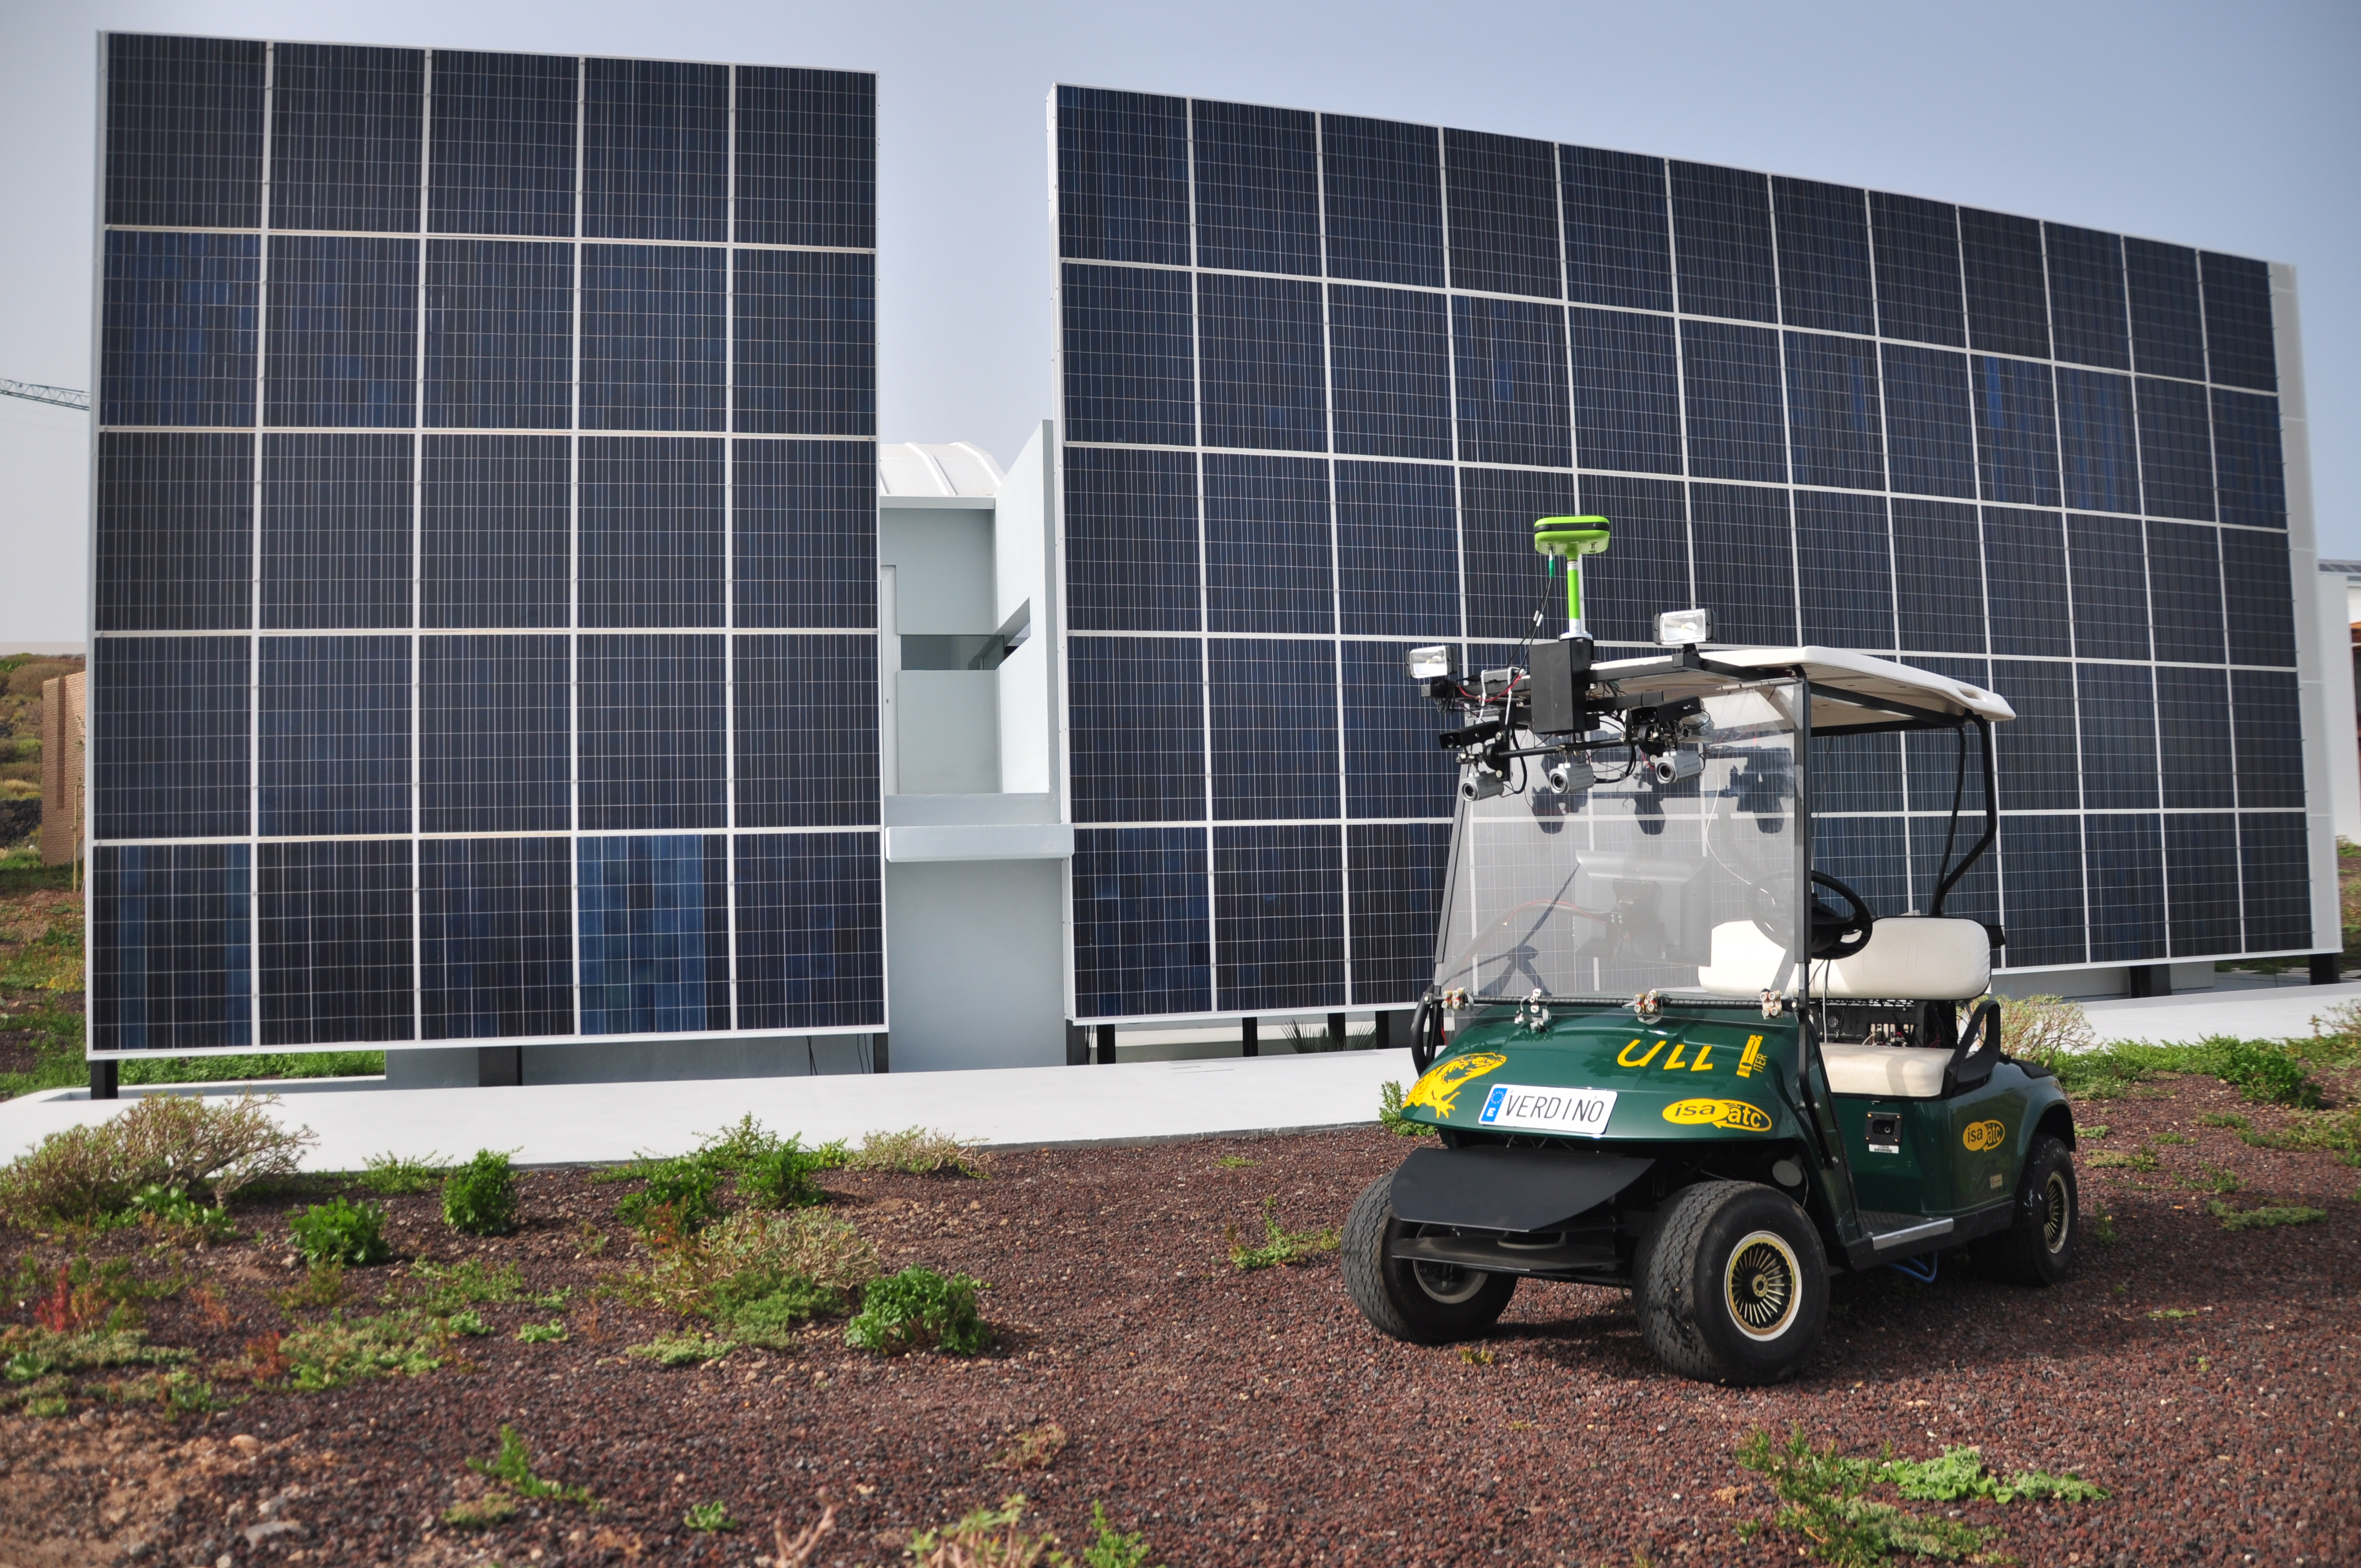
\includegraphics[height=\paperheight]{background}};\end{tikzpicture}}


% \setbeamercolor{alerted text}{fg=orange}
% \setbeamercolor{background canvas}{bg=green}
% \setbeamercolor{block body alerted}{bg=normal text.bg!90!black}
% \setbeamercolor{block body}{bg=normal text.bg!90!black}
% \setbeamercolor{block body example}{bg=normal text.bg!90!black}
% \setbeamercolor{block title alerted}{use={normal text,alerted text},fg=alerted text.fg!75!normal text.fg,bg=normal text.bg!75!black}
% \setbeamercolor{block title}{bg=blue}
% \setbeamercolor{block title example}{use={normal text,example text},fg=example text.fg!75!normal text.fg,bg=normal text.bg!75!black}
% \setbeamercolor{fine separation line}{}
% \setbeamercolor{frametitle}{fg=brown}
% \setbeamercolor{item projected}{fg=black}
% \setbeamercolor{normal text}{bg=black,fg=yellow}
% \setbeamercolor{palette sidebar primary}{use=normal text,fg=normal text.fg}
% \setbeamercolor{palette sidebar quaternary}{use=structure,fg=structure.fg}
% \setbeamercolor{palette sidebar secondary}{use=structure,fg=structure.fg}
% \setbeamercolor{palette sidebar tertiary}{use=normal text,fg=normal text.fg}
% \setbeamercolor{section in sidebar}{fg=brown}
% \setbeamercolor{section in sidebar shaded}{fg=gray}
% \setbeamercolor{separation line}{}
% \setbeamercolor{sidebar}{bg=red}
% \setbeamercolor{sidebar}{parent=palette primary}
% \setbeamercolor{structure}{bg=black, fg=green}
% \setbeamercolor{subsection in sidebar}{fg=brown}
% \setbeamercolor{subsection in sidebar shaded}{fg=gray}
% \setbeamercolor{title}{fg=brown}
% \setbeamercolor{titlelike}{fg=brown}

\defbeamertemplate*{footline}{shadow theme}
{%
  \leavevmode%
  \hbox{\begin{beamercolorbox}[wd=.5\paperwidth,ht=2.5ex,dp=1.125ex,leftskip=.3cm plus1fil,rightskip=.3cm]{author in head/foot}%
    \usebeamerfont{author in head/foot}\insertframenumber\,/\,\inserttotalframenumber\hfill\insertshortauthor
  \end{beamercolorbox}%
  \begin{beamercolorbox}[wd=.5\paperwidth,ht=2.5ex,dp=1.125ex,leftskip=.3cm,rightskip=.3cm plus1fil]{title in head/foot}%
    \usebeamerfont{title in head/foot}\insertshorttitle%
  \end{beamercolorbox}}%
  \vskip0pt%
}

%% Video stuff
\usepackage{movie15}

\AtBeginSubsection[]
{
  \begin{frame}
    \frametitle{Table of Contents}
    \tiny
    \tableofcontents[currentsection]
  \end{frame}
}

\begin{document}
\addtobeamertemplate{headline}{}{%
\begin{textblock*}{100mm}(0.2cm,-1.4cm)

\includegraphics[height=1.2cm]{verdino_logo}
\end{textblock*}}

\begin{frame}[plain]
    \begin{overlayarea}{\textwidth}{\textheight}
      \centering
      
  %     \includegraphics[height=0.5cm]{ull} \hspace*{0.5\textwidth}
  %     
\includegraphics[height=2cm]{verdino} 
  %     \begin{textblock*}{100mm}(0.02cm,-0.8cm)
  %       
\includegraphics[height=.7cm]{verdino}
  %     \end{textblock*}

      \titlepage
      
      \tiny
      \hfill Under the guidance of:\\
      \scriptsize
      \hfill Dr. Leopoldo Acosta Sánchez\\
      \hfill Dr. Jonay T. Toledo Carrillo
    \end{overlayarea}
    \begin{textblock*}{100mm}(-3.4cm,-1.5cm)
      
\includegraphics[height=5cm]{verdino_logo}
    \end{textblock*}
\end{frame}

% \section{chapter00} \begin{frame} Lalala \end{frame}
% \section{Obstacle Detection}
% \subsection{chapter01} \begin{frame} Lalala \end{frame}
% \subsection{chapter02} \begin{frame} Lalala \end{frame}
% \subsection{chapter03} \begin{frame} Lalala \end{frame}
% \subsection{chapter04} \begin{frame} Lalala \end{frame}
% \subsection{chapter05} \begin{frame} Lalala \end{frame}
% \section{Obstacle Avoidance and Planning}
% \subsection{chapter06} \begin{frame} Lalala \end{frame}
% \subsection{chapter07} \begin{frame} Lalala \end{frame}
% \section{Results} \begin{frame} Lalala \end{frame}
% \subsection{chapter01} \begin{frame} Lalala \end{frame}
% \subsection{chapter02} \begin{frame} Lalala \end{frame}
% \subsection{chapter04} \begin{frame} Lalala \end{frame}
% \subsection{chapter05} \begin{frame} Lalala \end{frame}
% \subsection{chapter06} \begin{frame} Lalala \end{frame}
% \subsection{chapter07} \begin{frame} Lalala \end{frame}
% \section{Conclusions} \begin{frame} Lalala \end{frame}

\graphicspath{{./images/bmps/}{./images/vects/}{./images/}
  {./images/presentation/bmps/}{./images/presentation/vects/}{./images/presentation/}
  {./images/chapter00/bmps/}{./images/chapter00/vects/}{./images/chapter00/}
  {./images/chapter01/bmps/}{./images/chapter01/vects/}{./images/chapter01/}
  {./images/chapter02/bmps/}{./images/chapter02/vects/}{./images/chapter02/}
  {./images/chapter03/bmps/}{./images/chapter03/vects/}{./images/chapter03/}
  {./images/chapter04/bmps/}{./images/chapter04/vects/}{./images/chapter04/}
  {./images/chapter05/bmps/}{./images/chapter05/vects/}{./images/chapter05/}
  {./images/chapter06/bmps/}{./images/chapter06/vects/}{./images/chapter06/}
  {./images/chapter07/bmps/}{./images/chapter07/vects/}{./images/chapter07/}
}

\section{Introduction}
%   \begin{frame}{Introduction}
%     \begin{itemize}
%       \item<1-> Humans should not drive.
%       \begin{itemize}
% 	\item<2-> Road injuries are one of the top-ten causes death, according to the World Health Organization (WHO).
% 	\note {Fortunately, the number of deaths for this cause has been reduced.}
% 	\note {Popularization of Advanced Driver Assistance Systems (ADAS) could be very related to this fact.}
% 	\item<3-> Driving is difficult, too.
% 	\note{An average US citizen expends 38 hours stuck in traffic.}
%       \end{itemize}
%       \item<4-> The amount of research related to autonomous vehicles has increased a lot.
%     \end{itemize}  
%     \begin{center}
%       \includegraphics<1-1>[height=.45\textheight]{CarCartoon}
%       \includegraphics<2-2>[height=.45\textheight]{WHO-data-10-deaths}
%       \includegraphics<3-3>[height=.45\textheight]{trafficsigns}
%       \includegraphics<4-4>[height=.45\textheight]{uav_research}
%     \end{center}
%   \end{frame}
  
%   \begin{frame}{Advantages of autonomous vehicles}
%     \begin{columns}[c] % the "c" option specifies center vertical alignment
%       \column{.5\textwidth} % column designated by a command
%       \begin{itemize}
% 	\item<1-> Higher safety.      
% 	\item<2-> Reduced traffic congestion.
% 	\item<3-> More free time.
% 	\item<4-> Higher speed limits.
% 	\item<5-> Occupant constraints.
% 	\item<6-> Parking problems.
% 	\item<7-> Traffic police.
% 	\item<8-> Vehicle insurance.
% 	\item<9-> Road signs.
% 	\item<10-> Smoother ride.
%       \end{itemize}  
%       \column{.5\textwidth}
%       \begin{center}
% 	\includegraphics<1-1>[width=\textwidth]{safety}
% 	\includegraphics<2-2>[width=\textwidth]{congestion}
% 	\includegraphics<3-3>[width=\textwidth]{freetime}
% 	\includegraphics<4-4>[width=\textwidth]{speedlimit}
% 	\includegraphics<5-5>[width=\textwidth]{stpatricks}
% 	\includegraphics<6-6>[width=\textwidth]{parking}
% 	\includegraphics<7-7>[width=\textwidth]{police}
% 	\includegraphics<8-8>[width=\textwidth]{insurance}
% 	\includegraphics<9-9>[width=\textwidth]{roadsign}
% 	\includegraphics<10-10>[width=0.8\textwidth]{smoothride}
%       \end{center}
%     \end{columns}
%     
%     \note {
%     \begin{itemize}
%       \item As said, higher safety due a to a decrease in the number of traffic accidents.
%       \item Reduced traffic congestion, as the roads can increase their capacity.
%       \item Vehicle occupants can spend their time in things other than driving.
%       \item Higher speed limits.
%       \item Occupants are not tied to constraints like being under age, blind, intoxicated, etc.
%       \item Alleviation of parking scarcity and reduction of space required for vehicle parking.
%       \item Reduction in the need for traffic police and vehicle insurance.
%       \item Physical road signs will not be needed anymore: autonomous cars could receive necessary communication electronically.
%       \item Smoother ride.
%     \end{itemize}
%     }
%   \end{frame}

  \subsection{Problem Statement}
  \begin{frame}{Problem Statement}
    \begin{itemize}
     \item<1-> We propose different methods which will be used for the detection and tracking of obstacles by our prototype, Verdino.
     \item<2-> These will be used by a global and a local planner for generating and following a safe path.
    \end{itemize}
    \begin{center}
      \includegraphics<1->[height=.35\columnwidth]{verdino}
    \end{center}
  \end{frame}
  
  \begin{frame}[plain]{Pipeline}
    \begin{center}
      \includegraphics[height=1.1\textheight]{pipeline_cp0}
    \end{center}
    
  \end{frame}

  
  \begin{frame}{Obstacle detection and tracking}
    \begin{itemize}
    \item<1-> Goals:
      \begin{enumerate}
      \item<2-> Good obstacle detection rate. 
      \item<3-> Obstacle localization.
      \item<4-> Real time.
      \item<5-> Environment conditions independence.
      \item<6-> Tracking capabilities.
      \item<7-> Moving cameras.
      \end{enumerate}
    \end{itemize}
  \end{frame}
  
%   \begin{frame}{Obstacle detection and tracking}
%     \begin{itemize}
%       \item <1-> We propose four different approaches:
%       \begin{enumerate}
% 	\item<1-> Change detection and image registration. 
% 	\item<2-> Background substraction and nonrigid point set registration.
% 	\item<3-> Stixels.
% 	\item<4-> Voxels and a particle filter.
%       \end{enumerate}
%     \end{itemize}
%       
%     \begin{center}
%       \includegraphics<1-1>[height=.3\columnwidth]{database}
%       \includegraphics<2-2>[height=.3\columnwidth]{fig6}
%       \includegraphics<3-3>[height=.3\columnwidth]{stixels_over_original}
%       \includegraphics<4-4>[height=.3\columnwidth]{fakePointCloud}
%     \end{center}
%   \end{frame}
  
  \begin{frame}{Obstacle Avoidance and Planning}
    We distinguish two different levels:
    \begin{enumerate}
     \item<1-> Global planning. 
     \item<2-> Local planning.
    \end{enumerate}

    \begin{center}
      \includegraphics<1-1>[height=.35\columnwidth]{figure7}
      \includegraphics<2-2>[height=.35\columnwidth]{example3a}
    \end{center}
  \end{frame}
  
  \begin{frame}{Evaluation of Stereo 3D Reconstruction Algorithms}
    Apart from the previous, we developed some methods intended to assess the performance of the 3D stereo reconstruction algorithms used for the particle filter based approach.
    
    \begin{center}
      \includegraphics[height=.4\columnwidth]{fc}
    \end{center}
    
  \end{frame}
    
  \subsection{Previous Work}
%   \begin{frame}{Autonomous vehicles review}
%     \begin{columns}[T] % the "c" option specifies center vertical alignment
%       \column{.5\textwidth} % column designated by a command
%       \footnotesize
%       \begin{itemize}
% 	\item<1-> \textbf{(1987-1995)} EC EUREKA Prometheus Project.
% 	\item<2-> \textbf{(1996)} ARGO Project.
% 	\item<3-> \textbf{(2004)} $1^{st}$ DARPA's Grand Challenge.
% 	\item<4-> \textbf{(2005)} $2^{nd}$ DARPA's Grand Challenge.
% 	\item<5-> \textbf{(2007)} DARPA's Urban Challenge.
% 	\item<6-> \textbf{(2010, 2012, 2013)} Korean Autonomous Vehicle Competition (AVC).
%       \end{itemize}  
%       \column{.5\textwidth}
%       \begin{center}
% 	\vskip -1cm
%        	\begin{overlayarea}{\textwidth}{\textheight}
% 	  \only<1>{
% 	  \begin{block}{EC EUREKA Project}
% 	    \begin{itemize}
% 	    \item VITA-2\\
% 	    \begin{center}\includegraphics<1->[width=0.5\textwidth]{vita2}\end{center}
% 	    \item VaMP\\
% 	    \begin{center}\includegraphics<1->[width=0.5\textwidth]{VaMP}\end{center}
% 	    \end{itemize}
% 	  \end{block}
% 	  }
% 	  \only<2>{
% 	  \begin{block}{ARGO Project}
% 	    \begin{itemize}
% 	      \item Lancia Thema.
% 	      \item Follow the lane marks of a road.
% 	      \item 1,900\,km
% 	      \item Average of 60\,Km/h.
% 	    \end{itemize}
% 	    \begin{center}\includegraphics<1->[width=0.5\textwidth]{argo}\end{center}
% 	  \end{block}
% 	  }
% 	  \only<3>{
% 	  \begin{block}{$1^{st}$ DARPA's Grand Challenge}
% 	    \begin{itemize}
% 	      \item Mojave Desert.
% 	      \item 240\,km route.
% 	      \item Listing of check points.
% 	      \item None finished the route.
% 	    \end{itemize}
% 	    \begin{center}\includegraphics<1->[width=0.5\textwidth]{urbanchallenge2004}\end{center}
% 	  \end{block}
% 	  }
% 	  \only<4>{
% 	  \begin{block}{$2^{nd}$ DARPA's Grand Challenge}
% 	    \begin{figure}[t]
% 		    \centering
% 		    \begin{subfigure}[b]{0.4\textwidth}
% 		      \includegraphics[width=\textwidth]{stanley}
% 		    \end{subfigure}
% 		    ~
% 		    \begin{subfigure}[b]{0.4\textwidth}
% 		      \includegraphics[width=\textwidth]{Sandstorm}
% 		    \end{subfigure}
% 		    \\~\\
% 		    \begin{subfigure}[b]{0.4\textwidth}
% 		      \includegraphics[width=\textwidth]{h1ghlander}
% 		    \end{subfigure}
% 		    ~
% 		    \begin{subfigure}[b]{0.4\textwidth}
% 		      \includegraphics[width=\textwidth]{kat5}
% 		    \end{subfigure}
% 		    \\~\\
% 		    \begin{subfigure}[b]{0.4\textwidth}
% 		      \includegraphics[width=\textwidth]{terramax}
% 		    \end{subfigure}
% 	    \end{figure}
% 	  \end{block}
% 	  }
% 	  \only<5>{
% 	  \begin{block}{DARPA's Urban Challenge}
% 	    \begin{figure}[t]
% 		    \centering
% 		    \begin{subfigure}[b]{0.4\textwidth}
% 		      \includegraphics[width=\textwidth]{boss}
% 		    \end{subfigure}
% 		    ~
% 		    \begin{subfigure}[b]{0.4\textwidth}
% 		      \includegraphics[width=\textwidth]{junior}
% 		    \end{subfigure}
% 		    \\~\\
% 		    \begin{subfigure}[b]{0.4\textwidth}
% 		      \includegraphics[width=\textwidth]{odin}
% 		    \end{subfigure}
% 		    ~
% 		    \begin{subfigure}[b]{0.4\textwidth}
% 		      \includegraphics[width=\textwidth]{talos}
% 		    \end{subfigure}
% 		    \\~\\
% 		    \begin{subfigure}[b]{0.4\textwidth}
% 		      \includegraphics[width=\textwidth]{littleben}
% 		    \end{subfigure}
% 		    ~
% 		    \begin{subfigure}[b]{0.4\textwidth}
% 		      \includegraphics[width=\textwidth]{skynet}
% 		    \end{subfigure}
% 
% 	    \end{figure}
% 	  \end{block}
% 	  }
% 	  \only<6>{
% 	  \begin{block}{Korean Autonomous Vehicle Competition (AVC)}
% 	    \includegraphics[width=\textwidth]{kavc}
% 	  \end{block}
% 	  }
% 	\end{overlayarea}
%       \end{center}
%     \end{columns}
%     
%     \note {
%     \begin{itemize}
%       \item From 1987 to 1995, the EC EUREKA Prometheus Project conducted research on autonomous vehicles. Among its culmination points were the twin robot vehicles VITA-2 and VaMP, driving long distances in heavy traffic.
%       \item In 1996, the ARGO project modified a Lancia Thema to follow the lane marks in an unmodified highway \citep{Broggi1999}. The culmination of the project was a journey of 1,900\,km over six days on the motorways of northern Italy, with an average speed of 90 km/h. The car operated in fully automatic mode for the 94\% of its journey, with the longest automatic stretch being 55\,km. The vehicle had only two grayscale low-cost video cameras on board and used stereoscopic vision algorithms to understand its environment. 
%       \item In 2004, DARPA's Grand Challenge was held in the Mojave Desert region of the United States, along a 240\,km route. This competition consisted on an autonomous vehicles race that must reach to the goal without human intervention and using just a listing of check points between the start and the finish line. None of the robot vehicles finished the route.
%       \item In 2005, a second competition was held \citep{Buehler2007}. This time, five vehicles successfully completed the course:
%       \begin{itemize}
%       \item \emph{Stanley} \citep{thrun2006stanley}, from Standford University.
%       \item \emph{Sandstorm} and \emph{H1ghlander} \citep{urmson2004high}, from the Carnegie Mellon University.
%       \item \emph{Kat-5} \citep{trepagnier2006kat}, from the Gray Insurance Company.
%       \item \emph{TerraMax} \citep{ozguner2004team}, from the Oshkosh Truck Corporation.
%       \end{itemize}
%       \item In 2007, the third driverless car competition of the DARPA Grand Challenge \citep{Buehler2009}, more known as the DARPA Urban Challenge, was held in Victorville, California. This time, six teams successfully finished the entire course:
%       \begin{itemize}
%       \item \emph{Boss} \citep{Urmson2008}, from the Carnegie Mellon University.
%       \item \emph{Junior} \citep{montemerlo2008junior}, from Standford University.
%       \item \emph{Odin} \citep{Bacha2008}, from Virginia Tech.
%       \item \emph{Talos} \citep{leonard2007team}, from the Massachusetts Institute of Technology.
%       \item \emph{Little Ben} \citep{bohren2008little}, from University of Pennsylvania.
%       \item \emph{Skynet} \citep{miller2008team}, from Cornell University.
%       \end{itemize}
%       \item In 2010, 2012 and 2013, the Korean Autonomous Vehicle Competition (AVC) took place.
%     \end{itemize}
%     }
%   \end{frame}
% 
%   \begin{frame}{Autonomous vehicles review}
%     \begin{columns}[T] % the "c" option specifies center vertical alignment
%       \column{.5\textwidth} % column designated by a command
%       \footnotesize
%       \begin{itemize}
% 	\item<1-> \textbf{(2010)} VIAC Challenge.
% 	\item<3-> \textbf{(2011)} WildCat Project.
% 	\item<4-> \textbf{(2011)} AutoNOMOS Group.
% 	\item<5-> \textbf{(2012)} Shelley.
% 	\item<6-> \textbf{(February 2013)} RobotCar project.
% 	\item<7-> \textbf{(July 2013)} BRAiVE.
% 	\item<8-> \textbf{(Nowadays)} Many working prototypes.
%       \end{itemize}  
%       \column{.5\textwidth}
%       \begin{center}
% 	\vskip -1cm
%        	\begin{overlayarea}{\textwidth}{\textheight}
% 	  \only<1-2>{
% 	  \begin{block}{VIAC Challenge}
% 	    \begin{itemize}
% 	    \item<1-> From Italy to China.
% 	    \item<1-> 100 day, 15,900\,km.
% 	    \item<2-> Four autonomous vehicles.
% 	    \item<2-> Limited human intervention.
% 	    \end{itemize}
% 	    \begin{center}
% 	      \includegraphics<1>[width=0.8\textwidth]{viacMap}
% 	      \includegraphics<2>[width=0.8\textwidth]{viacCars}
% 	    \end{center}
% 
% 	  \end{block}
% 	  }
% 	  \only<3>{
% 	  \begin{block}{WildCat Project}
% 	    \begin{itemize}
% 	      \item Bowler Wildcat.
% 	      \item Oxford University.
% 	    \end{itemize}
% 	    \begin{center}\includegraphics<1->[width=\textwidth]{wildcat}\end{center}
% 	  \end{block}
% 	  }
% 	  \only<4>{
% 	  \begin{block}{AutoNOMOS Group}
% 	    \begin{itemize}
% 	      \item Spirit of Berlin.\\
% 	      \begin{center}\includegraphics<1->[width=0.5\textwidth]{spiritofberlin}\end{center}
% 	      \item MadeInGermany.\\
% 	      \begin{center}\includegraphics<1->[width=0.5\textwidth]{madeingermany}\end{center}
% 	    \end{itemize}
% 	  \end{block}
% 	  }
% 	  \only<5>{
% 	  \begin{block}{Shelley}
% 	    \begin{itemize}
% 	      \item More than 160\,km/h
% 	    \end{itemize}
% 	    \begin{center}\includegraphics<1->[width=\textwidth]{shelley}\end{center}
% 	  \end{block}
% 	  }
% 	  \only<6>{
% 	  \begin{block}{RobotCar project}
% 	    \begin{itemize}
% 	      \item Oxford University.
% 	      \item Switches from manual to autopilot on learned routes.
% 	    \end{itemize}
% 	    \includegraphics[width=\textwidth]{robotcar}
% 	  \end{block}
% 	  }
% 	  \only<7>{
% 	  \begin{block}{BRAiVE}
% 	    \begin{itemize}
% 	      \item Vislab.
% 	      \item Moved on a mixed traffic route open to public traffic.
% 	    \end{itemize}
% 	    \includegraphics[width=\textwidth]{BRAiVE}
% 	  \end{block}
% 	  }
% 	  \only<8>{
% 	  \begin{block}{Many working prototypes}
% 	    \begin{figure}[t]
% 	      \centering
% 	      \begin{subfigure}[b]{0.2\textwidth}
% 		\includegraphics[width=\textwidth]{mercedes_benz}
% 	      \end{subfigure}
% 	      ~
% 	      \begin{subfigure}[b]{0.2\textwidth}
% 		\includegraphics[width=\textwidth]{gm}
% 	      \end{subfigure}
% 	      ~
% 	      \begin{subfigure}[b]{0.2\textwidth}
% 		\includegraphics[width=\textwidth]{continental}
% 	      \end{subfigure}
% 	      \\~\\
% 	      \begin{subfigure}[b]{0.2\textwidth}
% 		\includegraphics[width=\textwidth]{autoliv}
% 	      \end{subfigure}
% 	      ~
% 	      \begin{subfigure}[b]{0.2\textwidth}
% 		\includegraphics[width=\textwidth]{bosch}
% 	      \end{subfigure}
% 	      ~
% 	      \begin{subfigure}[b]{0.2\textwidth}
% 		\includegraphics[width=\textwidth]{nissan}
% 	      \end{subfigure}
% 	      \\~\\
% 	      \begin{subfigure}[b]{0.2\textwidth}
% 		\includegraphics[width=\textwidth]{toyota}
% 	      \end{subfigure}
% 	      ~
% 	      \begin{subfigure}[b]{0.2\textwidth}
% 		\includegraphics[width=\textwidth]{audi}
% 	      \end{subfigure}
% 	      ~
% 	      \begin{subfigure}[b]{0.2\textwidth}
% 		\includegraphics[width=\textwidth]{vislab_logo}
% 	      \end{subfigure}
% 	      \\~\\
% 	      \begin{subfigure}[b]{0.2\textwidth}
% 		\includegraphics[width=\textwidth]{oxforduni_logo}
% 	      \end{subfigure}
% 	      ~
% 	      \begin{subfigure}[b]{0.2\textwidth}
% 		\includegraphics[width=\textwidth]{google}
% 	      \end{subfigure}
% 	    \end{figure}
% 	  \end{block}
% 	  }
% 	\end{overlayarea}
%       \end{center}
%     \end{columns}
%     
%     \note {
%     \begin{itemize}
%       \item In 2010, inside the VIAC Challenge, four autonomous vehicles drove from Italy to China on a 100-day 15,900\,km trip with only limited human intervention (in traffic jams and when passing toll stations). At the time, this was the longest-ever journey conducted by an unmanned vehicle \citep{Broggi2010VIAC}.
%       \item In 2011, under the Oxford University's WildCat Project, a Bowler Wildcat based prototype is capable of autonomous operation using a flexible and diverse sensor suite.
%       \item In 2011, the Freie Universität Berlin, Led by the AutoNOMOS group, developed two autonomous cars - \emph{Spirit of Berlin} \citep{berlin2007spirit} and \emph{MadeInGermany} \citep{gohring2013semi} - to drive in the innercity traffic of Berlin in Germany. They were able to handle intercity traffic, traffic lights and roundabouts between the International Congress Centrum and the Brandenburg Gate.
%       \item In 2012, Stanford's Dynamic Design Lab, in collaboration with the Volkswagen Electronics Research Lab, produced Shelley, an Audi TTS designed for high speed (greater than 160\,km/h) on a racetrack course.
%       \item In February 2013, Oxford University unveiled the RobotCar UK project, an inexpensive autonomous car capable of quickly switching from manual driving to autopilot on learned routes.
%       \item In July 2013, Vislab worldpremiered BRAiVE, a vehicle that moved autonomously on a mixed traffic route open to public traffic \citep{grisleri2010braive}.
%       \item Currently, many major companies and research organizations have developed working prototype autonomous vehicles, including Mercedes-Benz, General Motors, Continental Automotive Systems, Autoliv Inc., Bosch, Nissan, Toyota, Audi, Vislab (University of Parma), Oxford University and Google.
%     \end{itemize}
%     }
%   \end{frame}
  
  \begin{frame}[plain]{Obstacle detection}
    \begin{overlayarea}{\textwidth}{\textheight}
      \only<1-7> {
	We can divide object tracking methods into two subcategories:
	\begin{itemize}
	  \item \emph{2.5D Solutions:} Different approaches:
	  \begin{itemize}
	    \item \emph{6D Vision.} \cite{franke20056d}
	    \item \emph{Dynamic stixels.} \cite{badino2009stixel, pfeiffer2011towards, pfeiffer2013exploiting, benenson2011stixels, benenson2012pedestrian, benenson2012fast}
	    \item \emph{Tracked image features.} \cite{barth2009estimating}
	    \item \emph{Sensor fusion.} \cite{wu2009collision}
	    \item \emph{Occupancy grids.} \cite{danescu2012particle}
	  \end{itemize} 
	  \item \emph{3D Solutions}
	  \begin{itemize}
	    \item \emph{Voxel grids.} \cite{broggi2013}
	    \item \emph{Adjacent stacks of cells} \cite{Moravec96robotspatial}
	  \end{itemize}
	\end{itemize}
      }
    \end{overlayarea}
    \begin{overlayarea}{\textwidth}{\textheight}
      \only<2> {
	\vspace{-4.5cm}
	\begin{block}{6D-Vision}
	  \begin{center}
	    \includegraphics[height=0.5\textheight]{6dvision}
	  \end{center}
	\end{block}
      }
      \only<3> {
	\vspace{-4.5cm}
	\begin{block}{Stixel World}
	  \begin{center}
	    \includegraphics[height=0.5\textheight]{stixels_over_original}
	  \end{center}
	\end{block}
      }
      \only<5> {
	\vspace{-3cm}
	\begin{block}{Occupancy grids}
	  \begin{center}
	    \includegraphics[width=\textwidth]{danescuPF}
	  \end{center}
	\end{block}
      }
      \only<6> {
	\vspace{-8.2cm}
	\begin{block}{Voxel Grids}
	  \begin{center}
	    \includegraphics[height=0.4\textheight]{vislabVoxel}
	  \end{center}
	\end{block}
      }
    \end{overlayarea}
    \note{
    Based on how much information they use, we can divide object tracking methods into two subcategories:
    \begin{itemize}
      \item \emph{2.5D Solutions:} They do not make use of the complete information provided by 3D points. Instead of that, they tend to use elevation maps composed of uniform size cells. Each cell just stores occupancy and height information. This is the kind of methods that, as described before, usually consider obstacles as being in contact with a flat ground.
      In these methods, tracking is performed before the complete reconstruction is done, in an intermediate point based on an specific feature. Depending on the feature used, we distinguishing different approaches:
      \begin{itemize}
	\item \emph{Use of the 3D point as feature.} An example of this is the so called 6D vision \citep{franke20056d}, in which the 3D stereo vision extracted information is combined with an efficient implementation of an optical flow in the image space based on a GPU. Relevant points are tracked using a Kalman filter.
	\item \emph{Dynamic stixels.} This approach has been longer discussed in section \ref{ch:chapter00_02_04}.
	\item \emph{Tracked image features.} An example is the work by \cite{barth2009estimating}. There, obstacles are represented as a rigid 3D point set which are tracked in terms of feature displacements and depth measurements.
	\item \emph{Sensor fusion.} \cite{wu2009collision} reconstruct the objects as cuboids from a stereo point cloud. In this process, position and speed values are improved to a very accurate value by the use of a radar along with stereo.
	\item \emph{Occupancy grids.} This is a very popular choice for tracking. An occupancy grid is a probabilistic map of the driving environment, which encodes the past and present knowledge from sensor data, and which can be updated dynamically when new information is available. These occupancy grids can be cartesian, with rectangular cells, polar, or even a relation between columns in an image and the disparity. An example of this is the method by \cite{danescu2012particle}, which has inspired part of the work described in chapter \ref{ch:chapter05}.
	Another advantage of the model based on an occupancy grid is that it makes easier a collaborative update of the grid, which allows the usage of data from several sensors and observers. Another simple example of occupancy grid is that described in chapter \ref{ch:chapter07}.
      \end{itemize} 
      \item \emph{3D Solutions:} Usually based on complex grid maps that use complete 3D information. Again, depending on how this grid is represented, we find 
      \begin{itemize}
	\item \emph{Octree connected cubes.} An example is the work by \cite{wurm2010octomap} or \cite{broggi2013}.
	\item \emph{Adjacent stacks of cells}, as described in \cite{Moravec96robotspatial} 
      \end{itemize}
    \end{itemize}
    }
  \end{frame}

%   \begin{frame}{Path planning}
%     \begin{itemize}
%       \item Classical methods \citep{hwang1992gross}
%       \item Heuristic methods \citep{masehian2007classic}
%       \item SVM based methods
%       \begin{itemize}
%        \item Global
% 	 \begin{itemize}
% 	  \item \cite{miura2006support}
% 	  \item \cite{yang2012safe}
% 	 \end{itemize}
%        \item Local
% 	\begin{itemize}
% 	  \item \cite{sarkar2008mobile}
% 	  \item \cite{tennety2009support}
% 	  \item \cite{qingyang2012local}
% 	\end{itemize}
%       \end{itemize}
%     \end{itemize}
%     
%     \note{
%       About classical methods, in general they can be considered as variations of some general approaches: Roadmap, Cell Decomposition, Potential Fields and Mathematical Programming. These methods are not mutually exclusive; in fact, a lot of approaches use combinations of them. A review of some classical methods can be checked out in \cite{hwang1992gross}.
%  
%       About heuristic methods, these are the answer given by researchers to the limitations of the classic methods. The most representative methods inside this classification are Probabilistic Roadmaps (PRM) \citep{kavraki1996probabilistic}, Rapidly Exploring Random Trees (RRT) \citep{lavalle2000rapidly}, Level set \citep{sethian1999level}, Linguistic Geometry (LG) \citep{stilman1993network}, Simulated Annealing (SA) \citep{zhu2006robot}, Artificial Neural Network (ANN) \citep{hossain2012real}, Genetic Algorithms (GA) \citep{zhang2007evolutionary}, Particle Swarm Optimization (PSO) \citep{chen2006smooth}, Ant Colony (ACO) \citep{mou2008modified} and its variants, like the RNA algorithm described in \cite{zhu2011new}, Stigmergy \citep{cazangi2006evolutionary}, Wavelet Theory \citep{doh2005systematic}, Fuzzy Logic (FL) \citep{kladis2011energy} and Tabu Search (TS) \citep{nguyen2012multi}. For more information, the review in \cite{masehian2007classic} can be checked.
%       
%       Global:
%       In the work presented by \cite{miura2006support}, navigation is planned in environments in which the obstacles are known. Obstacles are randomly labeled into two classes: positive or negative. Using these two classes, a SVM is trained and the decision boundary is used as a path. To increase the efficiency, a set of fake obstacles (guide samples) is generated at both sides of the current and goal position, as well as in parallel to the line that joins both points (nominal line), with the objective of helping the SVM to find a feasible path.
%       \cite{yang2012safe}. In their work, a preprocessing step is used in which the Voronoi Diagram is generated using the obstacles in the map. That diagram is used to select the best path between the starting point of the robot and the goal. The path obtained using Voronoi is not smooth, so the SVM is used to make this path smoother. The SVM is trained using a dataset in which the sites that generated the Voronoi edges are classified as positive or negative depending on their position (left / right) regarding to the previously obtained path. The decision boundary of this SVM will be the final path used.
%       
%       Local:
%       In \cite{sarkar2008mobile, tennety2009support}, authors divide the whole set of objects in the map into two classes and the SVM is used to determine the maximum margin hyperplane between the data sets belonging to the two classes. Data is assigned to one or another class depending on whether the points are on the left or on the right side of the robot. Once the initial labels are assigned, further classification is done using the k-nearest neighbor algorithm, with k=1.
%       \cite{qingyang2012local}, that uses a path subdivision method and a SVM. They use topological maps of local environments which are extracted with little expanded nodes. Next, candidate routes are optimized using the Support Vector Machine, where the candidate routes boundary points are defined as positive and negative samples. They also extend the original SVM \citep{cortes1995support} in order to satisfy extra constraints such as vehicle position and heading.
%     }
%   \end{frame}
%   
%     \begin{frame}{Local planning}
%     \begin{itemize}
%       \item \cite{werling2010optimal}
%       \item \cite{thrun2006stanley}
%       \item \cite{chu2012local}
%     \end{itemize}
%      
%     \note{
%       \begin{itemize}
% 	\item In \cite{werling2010optimal}, long term objectives are performed, like speed keeping, merging, following, stopping. This is done through optimal control strategies within the Fren\'et frame of the street.
% 	\item In \cite{thrun2006stanley}, lateral offset is defined as the perpendicular to an established base trajectory. This allows the vehicle driving along the road parallel to this trajectory. In order to select the optimal path, the cost function penalizes passing over obstacles and the distance respect to the center of the current road.
% 	\item In \cite{chu2012local}, also a set of candidate paths are generated, with endpoints in fixed positions at different offsets respect to the base frame, but they do not set this base frame in the center of the road, since it could be dangerous when computing the costs at certain scenarios. Instead of that, they use a security cost for each candidate path. Security of the path is computed by blurring the binary data of the obstacles. They also have into account certain criteria, as the smoothness cost or the path consistency between iterations.
%       \end{itemize}
%     }
%   \end{frame}
  
  \subsection{Testing platform}
  \begin{frame}{Testing platform}
    These algorithms are intended to be used in Verdino.
    \begin{itemize}
     \item<1-> Prototype developed by GRULL, Universidad de La Laguna.
     \item<2-> It will transport people around a bioclimatic urbanization in the ITER facilities.
     \item<3-> A golf cart has been modified to be used as an unmanned vehicle.
    \end{itemize}

    \begin{center}
      \includegraphics<1-1>[height=.3\columnwidth]{verdino}
      \includegraphics<2-2>[height=.3\columnwidth]{iter}
      \includegraphics<3-4>[height=.3\columnwidth]{NV_TXT2}
      \includegraphics<4-4>[height=.3\columnwidth]{verdino}
    \end{center}
  \end{frame}
  
%   \begin{frame}{Actuators}
%     \begin{columns}[c] % the "c" option specifies center vertical alignment
%       \column{.5\textwidth} % column designated by a command
%       \begin{itemize}
% 	\item<1-> Steering system.      
% 	\item<2-> Braking system.
% 	\item<3-> Speed system.
% 	\item<4-> Safety switch.
%       \end{itemize}  
%       \column{.5\textwidth}
%       \begin{center}
% 	\includegraphics<1-1>[width=\textwidth]{steering}
% 	\includegraphics<2-2>[width=\textwidth]{braking}
% 	\includegraphics<3-3>[width=\textwidth]{speedControl}
% 	\includegraphics<4-4>[width=\textwidth]{panicbutton}
%       \end{center}
%     \end{columns}
%     
%     \note {
%     \begin{itemize}
%       \item Steering system: we tied the original steering to a DC motor controlled by a PID.
%       \item Braking system: Controlled through a pneumatic system, composed by a cylinder, a commutation valve, two flow controllers and an air compressor. The pneumatic cylinder acts over the brake cables, that make pressure over the brake drums. A compressor gives the air pressure needed for this process.
%       \item Speed system: A microcontroller generates three different signals, that simulate the original devices installed in the vehicle. These correspond to a switch relay, which turns on the motor when the user pushes the acceleration pedal; the sense of speed (forward or backward); and the desired voltage
%       \item Safety switch: Allows changing between automatic and manual behavior. When switched off, the vehicle behaves as it was before the modifications.
%     \end{itemize}
%     }
%   \end{frame}
% 
%   \begin{frame}{Sensors}
%     \begin{columns}[c] % the "c" option specifies center vertical alignment
%       \column{.5\textwidth} % column designated by a command
%       \begin{itemize}
% 	\item<1-> Localization sensors.      
% 	\begin{itemize}
% 	  \item<3-> Odometry.      
% 	  \item<4-> IMU.
% 	  \item<5-> Differential GPS.
% 	\end{itemize}  
% 	\item<2-> Navigation sensors.	
% 	\begin{itemize}
% 	  \item<6-> LIDAR.      
% 	  \item<7-> IR cameras.
% 	  \item<8-> Visible cameras.
% 	\end{itemize}
%       \end{itemize}  
%       \column{.5\textwidth}
%       \begin{center}
% 	\includegraphics<3-3>[width=\textwidth]{odometry}
% 	\includegraphics<4-4>[width=\textwidth]{imu}
% 	\includegraphics<5-5>[width=\textwidth]{dgps}
% 	\includegraphics<6-6>[width=\textwidth]{lidar}
% 	\includegraphics<7-7>[width=\textwidth]{ircameras}
% 	\includegraphics<8-8>[width=\textwidth]{visiblecamera}
%       \end{center}
%     \end{columns}
%     
%     \note {
%     \begin{itemize}
%       \item \emph{Odometry}: This system measures the independent movement of the two rear wheels, which are attached to an optical encoder. This allows computing the position, orientation and speed of the prototype incrementally.
%       \item \emph{IMU}: It is comprised by 9 sensors (3 accelerometers, 3 gyroscopes and 3 magnetometers), which are fused in real time in order to get the three-dimensional orientation of the vehicle. The model of the sensor is a \emph{Xsens Mti}.
%       \item \emph{DGPS}: Allows positioning the vehicle with centimetric accuracy. It is composed by two different devices, the reference station, which is fixed in a known place, and the rover station, which is installed on the vehicle. The model used is a \emph{JAVAD GNSS Triumph-1}, which has an horizontal precision below 1\,cm and a vertical precision around 1.5\,cm using DGPS, at a frequency of $5\,Hz$.
%       \item \emph{LIDAR}: These are used also for localization purposes. Each of those sensors is able to detect the objects in the way of the vehicle, at the plane in which the sensor is mounted. The advantages of these sensors are that they have a high speed and precision. However, they are just able to detect obstacles that crosses the plane defined by the sensor. Because of this, we have equipped the vehicle with 5 LIDAR. Two of them are located at the same plane in the front corners of the vehicle, at a height of 50\,cm. Each of these covers an angle of 270\textdegree. Another is located in the front side of the vehicle, at a height of 20\,cm, slightly tilted upwards, in order to detect the small obstacles or non traversable areas. Another is in the top of the vehicle, also in the front side of the vehicle, tilted to the ground and covering the blind areas left by the other sensors. Finally, the last sensor is situated in the back side of the vehicle, and it is used for backwards maneuvers. The used sensors are of the model \emph{SICK LMS 100} and \emph{SICK LMS 111}, allowing a maximal detection distance of 20\,m, a precision of 10-35\,mm, a maximal angular resolution of 0.25\textdegree and a maximal rate of $50\,Hz$.
%       \item \emph{IR cameras}: Infrared cameras are used to detect pedestrians or animals based on their temperature. We have a pair of them installed on a Pan-Tilt system attached to the top front side of the vehicle. The model used is a \emph{MobiR\textregistered~M3}, which is able to detect objects in the range $8\sim14\mu m$, at a resolution of $160 \times 120\,px$.
%       \item \emph{Visible cameras}: A set of three cameras is also installed in a pan-tilt structure. These are used for the detection and tracking of the objects, which is one of the goals of this thesis. Also, they are currently being used for the detection of the borders of the road. The model of the cameras is a \emph{GoPro\textregistered Hero 3 silver edition}, with a $1920 \times 1080 \, px$ maximal video resolution and a 170\textdegree field of view at a maximal rate of 60\,fps.
%     \end{itemize}
%     }
%   \end{frame}
%   
%   \begin{frame}{Control}
%     \begin{columns}[c] % the "c" option specifies center vertical alignment
%       \column{.5\textwidth} % column designated by a command
%       \begin{itemize}
% 	\item Onboard computer.   
% 	\begin{itemize}
% 	  \item i7-3770K.      
% 	  \item 16 Gb RAM DDR3.
% 	  \item SSD Storage.
% 	\end{itemize}	
% 	\item Low-level control.
%       \end{itemize}  
%       \column{.5\textwidth}
%       \begin{center}
% 	\includegraphics[width=\textwidth]{onboard}
%       \end{center}
%     \end{columns}
%     
%     \note {
%     The vehicle is controlled, at high level, by an on board computer equipped with an \emph{i7-3770K} processor, 16\,Gb of \emph{RAM DDR-3} memory and a \emph{SSD} storage. At low level, a set of own developed electronic devices receive commands from the computer and transform them into the right signal, understandable by the actuators described before.
%     }
%   \end{frame}
  
\section{Obstacle Detection}
%%
%%  chapter01.tex - Obstacle Detection and Planning for Autonomous Vehicles based on Computer Vision Techniques
%%
%%  Copyright 2014 Néstor Morales <nestor@isaatc.ull.es>
%%
%%  This work is licensed under a Creative Commons Attribution 4.0 International License.
%%

\chapter{Problem Statement}\label{ch:chapter01}

\section{Problem Statement}\label{ch:chapter01_01}

Computer Vision environment understanding targeted at enabling autonomous operation of a robotic platform has been widely studied over the years, leading to the creation of some prototype vehicles \cite{Maurer1996,Pomerleau1996,Broggi1999} which demonstrated that negotiating moderately complex and dynamic situations in real time was possible, albeit challenging. However, it was only with the development effort driven by the DARPA Challenges \cite{Buehler2007, Buehler2009} that the technology required to provide reliable operation both in off-road and urban scenarios proved to be within reach.
The vehicles that successfully took part to this series of events had to integrate planning and actuation capabilities with a sensing suite capable of coping with harsh environments, heavy traffic and wide temperature ranges, while keeping functional over extended amounts of time. Most competitors relied on high-end active sensors \cite{Urmson2008, Montemerlo2008, Bacha2008, Kammel2008}, with some notable exceptions \cite{Broggi2006, Broggi2010}. 

As we discover when looking up to the available literature (See next section, \ref{ch:chapter01_02}), there are many methods for the detection and tracking of obstacles in complex environments, like this for which Verdino is intended to be working. In this sense, a very first approach is that inspired on the work by \cite{primdahl2005change},  \cite{diego2011video} or \cite{vallespi2012prior} was developed. This is based on the fact that, in an image, a high percentage of the scene represented usually corresponds to static objects. Based on that, it looks quite straightforward to think that, having an image representing an area without obstacles, it is possible to detect the obstacles in an scene by just comparing it with an image being taken in real time. For that, we obtained a dataset with geo-referenced images from a closed urbanization taken at different times of the day. A description of this database, as well as of the algorithm pipeline used for the comparison between images pairs can be found at section \todo{ \ref{XXX} }.

However, such approach suffers from several drawbacks. First, as we just use one image per frame, we are no able to know the exact position of the obstacle in the real world \comment{(Anyway, we think that the output of the algorithm is a good starting point for a classification method)}. Also, the quality of detection is highly tied to the size of the image database, so in big areas we need a huge dataset, with the related space and throughput problems associated to that. If we consider changes due to weather or light conditions, this dataset grows exponentially. Finally, we don't know the direction where an obstacle is going to. These are challenging problems that have been solved using different approaches, until we reached a final solution, described in section \todo { \ref{XXX} }.

To solve that, we first developed a method that tries to isolate just the tracking problem with the use of static monocular cameras. Instead of registering pairs of images, we segment the image with the use of foreground extraction techniques, distinguishing between background and foreground. Using the silhouette of the objects in the foreground (which are mainly non-rigid objects, like pedestrians or animals), we apply a non-rigid point set registration algorithm in order to track the different parts of the body of the obstacles separately. This method, inspired in works like those by \cite{starck2007surface}, or \cite{letouzey2011scene}, can be also used for the completion of the global map of the vehicle, or even for tasks more related to \acf{HMI}. This approach is extensively described in section \todo{ \ref{XXX}}.

However, this method still makes use of a very rudimentary method for the localization of the obstacles (See section \todo{ \ref{XXX-subsection_localization}}), and it is limited to static cameras. For the application proposed, we need the cameras installed on the top of the moving prototype, so we can not use foreground segmentation methods anymore for the detection of the objects in the road. A simple solution for that is stop using monocular vision, and start using stereo vision. In the last years, a high number of advanced algorithms has become viable for autonomous driving applications. The problem is that performing a quantitative and meaningful comparison of their performance level, however, is not an easy task, mainly because of the difficulty of producing ground truth information. Older datasets are small, and either synthetic or taken in controlled environments (\cite{Scharstein2002}), thus effectively limiting their usefulness as indicators of the actual algorithms ability to cope with outdoor scenarios. Due to that, it is needed to compare the performance level of some state-of-the-art stereovision-based 3D mapping algorithms in automotive scenarios. This evaluation methodology and the associated results is shown in section \todo{ \ref{XXX}}. \comment{PREGUNTAR A LA GENTE DEL VISLAB SI ESTA DE ACUERDO CON QUE USE ESTO EN LA TESIS, POR SI LAS MOSCAS}.

\comment{Este párrafo y la sección asociada dependerá de lo que consiga sacar más adelante.}\notsure{
Apart from the full-dense 3D reconstruction methods, we also explore the possibility of using a simpler (and faster) reconstruction based on Stixels, like that described by \cite{badino2009stixel}. In particular, we decided to use the implementation by \cite{benenson2012pedestrian}, due to its fast response (about 100 frames per second). The method, described in section \todo{\ref{XXX}}, compares the stixels obtained between frames and tracks the obstacles along the time. This solves all the problems we had: we can use moving cameras, we can locate the obstacles in the map, and also we are able to know the path followed by them.}

Another approach, which makes use of the dense stereo reconstruction algorithms for which we did the evaluation described above, is inspired in the work by \cite{danescu2010particle}, but also from the voxelized world described in \cite{broggi2013}. The key idea is to simplify the 3d reconstructed world into a grid of voxels, each of these representing a certain volume in the world. In this voxelized world, for each voxel above a given occupancy probability threshold, a set of particles part of a particle filter is assigned. Each particle will have a double function: the first, denoting hypotheses (as in the classical particle filter methods); the second, to be used as segmentation criteria in the segmentation of the world into different obstacles. In this way, we consider that two contiguous voxels belong to different obstacles if their obtained direction and sense diverges. A more detailed explanation of the method is found in \todo{\ref{XXX}}.

At this point, we have an acceptable reconstruction of the surroundings of the vehicle, which includes the localization and tracking of the obstacles in the neighborhood of the cart. But the reconstruction of the environment is not the only challenge that an autonomous vehicle has to deal with. Once that a vehicle has an idea of where it is, and where it wants to go, it also needs to know the best way to reach there and, more important, how to avoid the harmful elements it has previously detected using the methods described. This allows a safe trip, both for the pedestrians, cars, etc. in the road, and for the vehicle itself.
As said, Verdino is intended to travel in pedestrian areas where most of the obstacles are pedestrians, so its behavior must be mainly reactive in order to give priority to the safety of paths against the efficiency of the route. Also, there is not a clear traveling path, like a road. Instead of that, the vehicle will be moving around an unstructured area, so there is not something like a \acf{RNDF} that allows a fast calculation of the paths that the car will use to reach a certain point. Because of that, we must consider two different planning levels:
\begin{itemize}
 \item \textbf{Global Planning:}
 As it is not possible to determine a global trajectory based on a \acs{RNDF}, we must use a method able to deal with changing environments for the calculation of a fast and safe path. The idea is that, having a map of the static obstacles in the environment and with the vehicle properly localized on it \cite{Perea2013mcl}, it will generate a path that will allow reaching this destination as fast as possible. This task, which can be solved easily in static environments using graphs or other similar optimization methods, becomes a little bit more challenging in environments like, for example, a parking lot, in which cars are parking and driving off continuously.
 In section \todo{ \ref{XXX} }, the way in which we solved this problem is described. It is based on the border between classes, which is obtained after training a \acf{MSVM} (See Appendix \todo {\ref{XXX}} for more information), considering each single obstacle as a separate class. Instead of using this border for classification purposes, as it is usual, we take advantage of the fact that it will be the safest and smoother distance to the obstacles. Taking this into account, it makes sense to apply this separation line as our path. Also, the use of a different class for each obstacle allows ensuring that the path is safe enough, even in complicate scenarios, like in pedestrian areas.
 
 \item \textbf{Local Planning:}
 In a lower level, we also need a way to make the vehicle know how to follow the generated path. This problem requires a system able to, several times per second, calculate the best steering angle and speed in order to follow the global plan while avoiding the surrounding obstacles. The method, which is inspired in the work of \cite{chu2012local}, receives as input the current position of the vehicle in the map, its orientation, speed and the steering angle. Also, we provide it with the global plan obtained in the upper level. Finally, a map of the dynamic obstacles in the surrounds of the cart is computed and passed to the algorithm.
 
 This dynamic map can be filled with the information provided by sensors like \acp{LIDAR}, among other sensors. But it can can also be computed with the information extracted from cameras, and this is the connection point with the work described in the first part of this Thesis. The detected obstacles are included in the map, so the vehicle is able to avoid them using the calculated steering angle and speed.
 
 The way in which both this map and the speed/steering angle commands is obtained is described in section \ref{XXX}.
\end{itemize}
 
 The whole pipeline of the application developed for this thesis is shown at figure \ref{fig:cp01_pipeline}. 
 
 \begin{figure}[thb]\label{fig:cp01_pipeline}
      \centering
      \includegraphics{pipeline}
      \caption{Pipeline of the modules described in this Thesis.}
\end{figure}

From the images captured in real-time, obstacles are located and passed to the module in charge of the generation of the dynamic costmap. At the same time, the static map is used for the generation of a feasible trajectory. Using the current position and vehicle status, the local planner tries to compute the proper commands in order to follow the global plan while trying to avoid the obstacles included in the dynamic costmap.

\section{Previous Work}\label{ch:chapter01_02}

Research on autonomous vehicles is a task being developed for a long time and for which a big effort has been carried on. A proof of that is the extensive literature existing about that topic, in special since the first of the DARPA Challenges (\cite{Buehler2007, Buehler2009}). Since then, the literature related to the topic has increased. Also, the interest on the use of Computer Vision in autonomous vehicles is growing, due to the possibilities that images offer when compared to other sensors, like \acp{LIDAR}.
In 1996, the ARGO project... \todo{Continuar desde aquí, una vez tenga una especie de historia de los vehiculos autonomos, en la intro.}
\todo{TerraMax, VIAC, Braive, Annieway y cualquier otro que pille por el camino.}
As depicted from section \ref{ch:chapter01_01}, the topics described in this thesis are quite diverse, so it is fair to review the state-of-the art of each of these topics separately.

\subsection{Change detection for obstacle localization in images}\label{ch:chapter01_02_01}

blah blah blah blah blah blah blah blah blah blah blah blah blah blah blah blah blah blah blah blah blah blah blah blah blah blah blah blah blah blah blah blah blah blah blah blah blah blah blah blah blah blah blah blah blah blah blah blah blah blah blah blah blah blah blah blah blah blah blah blah blah blah blah blah blah blah blah blah blah blah blah blah blah blah blah blah blah blah blah blah blah blah blah blah blah blah blah blah blah blah blah blah blah blah blah blah blah blah blah blah blah blah blah blah blah blah blah blah blah blah blah blah blah blah blah blah blah blah blah blah blah blah blah blah blah blah blah blah blah blah blah blah blah blah blah blah blah blah blah blah blah blah blah blah blah blah blah blah blah blah blah blah blah blah blah blah blah blah blah blah blah blah blah blah blah blah blah blah 

\subsection{Non-rigid point set registration for obstacle tracking}\label{ch:chapter01_02_02}

blah blah blah blah blah blah blah blah blah blah blah blah blah blah blah blah blah blah blah blah blah blah blah blah blah blah blah blah blah blah blah blah blah blah blah blah blah blah blah blah blah blah blah blah blah blah blah blah blah blah blah blah blah blah blah blah blah blah blah blah blah blah blah blah blah blah blah blah blah blah blah blah blah blah blah blah blah blah blah blah blah blah blah blah blah blah blah blah blah blah blah blah blah blah blah blah blah blah blah blah blah blah blah blah blah blah blah blah blah blah blah blah blah blah blah blah blah blah blah blah blah blah blah blah blah blah blah blah blah blah blah blah blah blah blah blah blah blah blah blah blah blah blah blah blah blah blah blah blah blah blah blah blah blah blah blah blah blah blah blah blah blah blah blah blah blah blah blah 

\subsection{Evaluation of stereo 3D reconstruction algorithms}\label{ch:chapter01_02_03}

blah blah blah blah blah blah blah blah blah blah blah blah blah blah blah blah blah blah blah blah blah blah blah blah blah blah blah blah blah blah blah blah blah blah blah blah blah blah blah blah blah blah blah blah blah blah blah blah blah blah blah blah blah blah blah blah blah blah blah blah blah blah blah blah blah blah blah blah blah blah blah blah blah blah blah blah blah blah blah blah blah blah blah blah blah blah blah blah blah blah blah blah blah blah blah blah blah blah blah blah blah blah blah blah blah blah blah blah blah blah blah blah blah blah blah blah blah blah blah blah blah blah blah blah blah blah blah blah blah blah blah blah blah blah blah blah blah blah blah blah blah blah blah blah blah blah blah blah blah blah blah blah blah blah blah blah blah blah blah blah blah blah blah blah blah blah blah blah 

\subsection{Stixel World}\label{ch:chapter01_02_04}

blah blah blah blah blah blah blah blah blah blah blah blah blah blah blah blah blah blah blah blah blah blah blah blah blah blah blah blah blah blah blah blah blah blah blah blah blah blah blah blah blah blah blah blah blah blah blah blah blah blah blah blah blah blah blah blah blah blah blah blah blah blah blah blah blah blah blah blah blah blah blah blah blah blah blah blah blah blah blah blah blah blah blah blah blah blah blah blah blah blah blah blah blah blah blah blah blah blah blah blah blah blah blah blah blah blah blah blah blah blah blah blah blah blah blah blah blah blah blah blah blah blah blah blah blah blah blah blah blah blah blah blah blah blah blah blah blah blah blah blah blah blah blah blah blah blah blah blah blah blah blah blah blah blah blah blah blah blah blah blah blah blah blah blah blah blah blah blah 

\subsection{3D object tracking}\label{ch:chapter01_02_05}

By processing the data captured by sensors, it is desired to obtain the position, speed and size of an obstacle. However, usually sensors don't provide this information, so we need to process the information over time and do the tracking of detected obstacles. Many approaches that try to solve this problem, like \cite{danescu2012particle}, assume that obstacles have an standard geometry, and they are modeled as cuboids with associated position, size and speed vectors. This assumption is mostly correct in environments like highways, country roads, and certain urban scenarios, in which almost all the obstacles are cars, trucks or buses which can be simplified as cuboids. Also, these approaches tend to consider a flat ground.
However, this assumption cannot always done, as happens in pedestrian areas, intersections, off-road... In this case, we need to deal with specific shapes, sometimes with concave surfaces. The problem with this kind of obstacles is that methods that assume cuboid-shaped objects tend to wrap the obstacles with a convex shape, which causes an overestimation of their volume (\cite{broggi2013}). Another problem are those objects that are not laying on the ground, as happens with hanged traffic lights, tree crowns, lamps, etc. Usually, they are integrated into an occupancy grid as if they were touching the ground. About the ground plane assumption, in cases like that of an off-road scenario, it is important to estimate the real slope of the road in order to get good results.
Based on how much information they use, we can divide object tracking methods into two subcategories:
\begin{itemize}
 \item \emph{2.5D Solutions:} They do not make use of the complete information provided by 3D points. Instead of that, they tend to use elevation maps composed of uniform size cells. Each cell just stores occupancy and height information. This is the kind of methods that, as described before, usually consider obstacles as being in contact with a flat ground.
 In these methods, tracking is done before the complete reconstruction is done, in an intermediate point based on an specific feature. Based on this intermediate feature, we can distinguishing different kind of approaches:
  \begin{enumerate}
   \item \emph{Use of the 3D point as feature.} An example of this is the so called 6D vision (\cite{franke20056d}), in which the 3D stereo vision extracted information is combined with an efficient implementation of an optical flow in the image space based on a \acf{GPU}. Relevant points are tracked using a Kalman filter.
   \item \emph{Dynamic stixels.} \todo{This approach has been longer discussed in section \ref{ch:chapter01_02_04}.}\comment{Cambiar en caso de que al final no meta los stixels}
   \item \emph{Tracked image features.} As example, check the work by \cite{barth2009estimating}. In this work, obstacles are represented as a rigid 3D point set which are tracked in terms of feature displacements and depth measurements.
   \item \emph{Sensor fusion.} \cite{wu2009collision} reconstruct the objects as cuboids from a stereo point cloud. In this process, position and speed values are improved to a very accurate value by the use of a radar along with stereo.
   \item \emph{Occupancy grids.} This is a very popular choice for tracking. An occupancy grid is a probabilistic map of the driving environment, which encodes the past and present knowledge from sensor data, and which can be updated dynamically when new information is available. These occupancy grids can be cartesian, with rectangular cells, polar, or even a relation between columns in an image an the disparity. An example of this is the method by \cite{danescu2012particle}, which has inspired part of the work described in section \todo { \ref{XXX}}.
   Another advantage of the model based on an occupancy grid is that it makes easier a collaborative update of the grid, which allows the usage of data from several sensors and observers.
  \end{enumerate} 
 \item \emph{3D Solutions:} Usually based on complex grid maps that use complete 3D information. Again, depending on how this grid is represented, we find 
 \begin{enumerate}
   \item \emph{Octree connected cubes.} An example is the work by \cite{wurm2010octomap} or \cite{broggi2013}.
   \item \emph{Adjacent stacks of cells}, as described in \cite{Moravec96robotspatial} 
 \end{enumerate}
\end{itemize}

\subsection{Global planning}\label{ch:chapter01_02_06}

blah blah blah blah blah blah blah blah blah blah blah blah blah blah blah blah blah blah blah blah blah blah blah blah blah blah blah blah blah blah blah blah blah blah blah blah blah blah blah blah blah blah blah blah blah blah blah blah blah blah blah blah blah blah blah blah blah blah blah blah blah blah blah blah blah blah blah blah blah blah blah blah blah blah blah blah blah blah blah blah blah blah blah blah blah blah blah blah blah blah blah blah blah blah blah blah blah blah blah blah blah blah blah blah blah blah blah blah blah blah blah blah blah blah blah blah blah blah blah blah blah blah blah blah blah blah blah blah blah blah blah blah blah blah blah blah blah blah blah blah blah blah blah blah blah blah blah blah blah blah blah blah blah blah blah blah blah blah blah blah blah blah blah blah blah blah blah blah 

\subsection{Local planning}\label{ch:chapter01_02_03}

blah blah blah blah blah blah blah blah blah blah blah blah blah blah blah blah blah blah blah blah blah blah blah blah blah blah blah blah blah blah blah blah blah blah blah blah blah blah blah blah blah blah blah blah blah blah blah blah blah blah blah blah blah blah blah blah blah blah blah blah blah blah blah blah blah blah blah blah blah blah blah blah blah blah blah blah blah blah blah blah blah blah blah blah blah blah blah blah blah blah blah blah blah blah blah blah blah blah blah blah blah blah blah blah blah blah blah blah blah blah blah blah blah blah blah blah blah blah blah blah blah blah blah blah blah blah blah blah blah blah blah blah blah blah blah blah blah blah blah blah blah blah blah blah blah blah blah blah blah blah blah blah blah blah blah blah blah blah blah blah blah blah blah blah blah blah blah blah 

\section{Summary}\label{ch:chapter01_03}

In this chapter, we have described a general idea of the work presented in this Thesis. Also, the pipeline of the final developed application is introduced. All this information will be explained in more detail in the following sections, including implementation details together with some results and a discussion of the advantages/disadvantages of the different methods.


%%
%%  chapter02.tex - Obstacle Detection and Planning for Autonomous Vehicles based on Computer Vision Techniques
%%
%%  Copyright 2014 Néstor Morales <nestor@isaatc.ull.es>
%%
%%  This work is licensed under a Creative Commons Attribution 4.0 International License.
%%

\graphicspath{{./images/chapter02/bmps/}{./images/chapter02/vects/}{./images/chapter02/}}

\chapter{Change detection for obstacle localization in images}\label{ch:chapter02}

We drive by mind. That is, once we learn the path to go from a point $A$ to another point $B$, we follow that path without almost thinking. Even more, if a person does this way repeatedly and every day, there will be a day in which he will be able to memorize each black spot, each traffic light and even each pothole. So it is not difficult for us to be surprised the day in which they change the signals or the sense of a road.
Following this line of thought, we have developed a system in which we make our prototype to \emph{learn} the environment of a certain road, making it able to detect the changes. However, in our case, the changes in which we are interested are the obstacles in the way of the vehicle, giving it the ability to avoid them or to stop if necessary. The idea behind this system is having a dataset with images that have localization information associated. These images will be compared with those captured in real time by the on board cameras. Both images will be registered and changes detected, letting us to know the presence of obstacles or other changes that appeared since the stored images were captured.

This is done through the pipeline shown at figure \ref{fig:cp02_pipeline}. First, the database is captured offline. Then, in real time, images are aligned trough a typical image registration pipeline(feature localization, matching of the features between the images, image transformation and resampling). With the images aligned,  obstacles are retrieved.

\begin{figure}[thb]
  \centering
  \includegraphics{pipeline}
  \caption{Pipeline of the method.}
  \label{fig:cp02_pipeline}
\end{figure}

\section{The Method}\label{ch:chapter02_01}

In this section, we will describe each of the stages in the pipeline of the application, starting from the database generation and finishing with the detected obstacles. 

As said, the process is based on the generation of an image database in which each image is associated with certain meta-information, of which a big part is related to its position in the map, so the first step in the application is the development of a database covering the driving area. In this stage, the vehicle will be traveling inside the covered area, driven by a human or in controlled circumstances. While the vehicle is driven, the system stores images, which will have associated geographic information: \emph{latitude}, \emph{longitude}, \emph{height} and their transformation into $x$, $y$, $z$ and orientation coordinates with respect to the coordinates frame of the local map of the prototype. Other information that could be outstanding in the future is also stored (i.e., the day and the hour in which the image was taken, \ac{GPS} rms value, etc.). Images are pre-processed to have as information as possible when used in the next phase, reducing the execution times. For example, we get the set of features from the images offline, not in the real time application. With a $5\,Hz$ update rate, an image is stored about each meter traveled, depending on the speed of the vehicle. In this phase, there would not be any obstacle in the road where the car is going to drive. If so, in the later phase in which the images are processed to get the obstacles, fake objects are going to be detected, due to those obstacles recorded in the database image. Once this process is finished, there will be a database with geographically located images. In figure \ref{fig:cp02_image_database}, a composition of the testing area with some of the stored images highlighted is shown.

\begin{figure}[thb]
  \centering
  \includegraphics{database}
  \caption{Area covered by the database with some example images superimposed.}
  \label{fig:cp02_image_database}
\end{figure}

In real time, the vehicle starts driving by itself. Along the path, it passes over different positions near the recorded route. These positions are being reported by the \ac{GPS} device and transformed to the local coordinates to work easily with them. Simultaneously, an image is obtained from the camera while the system looks for the nearest image in the database. The current frame $I_{RT}$ and the image retrieved from the database $I_{DB}$ are compared by using image change detection techniques, obtaining the obstacles in the scene.

In the moment of the development of this application, localization was entirely retrieved from the \ac{GPS} device. This gave a position each 200 ms, so it was desirable to be able to process each frame under this time, in an on board 2009 PC computer.

\subsection{Image selection from database}\label{ch:chapter02_01_01}

This step is important as we want to get an image as similar as possible to the current real time image. This will affect to the quality of the adjustment between the images. Most of the times we just need to find an image with the smaller Euclidean distance to the current point, checking that the angular difference is not too big. Although this solution has good results, many times it is better to have an image not so close to the current point, if it means that all the objects represented in an image are going to appear in the other one. This can be got if an image which is forward or backward regarding to the current image is selected, so one of the images will be contained into the other. Doing that, it will reduce not just the angular difference, but also the lateral distance (which is usually the source of the misalignments due to an excess of parallax).

In figure \ref{fig:cp02_nearest_image}, we can observe this procedure. Based on this, the nearest image in the database is that obtained by the expression:

\begin{equation}\label{eq:cp02_nearest_image}
I^*_{DB} = \underset{I_{DB}}{\arg\min} \|p_{RT} - p_c\| = {{y_{RT} \cdot v_{DB_x} + x_{RT} \cdot v_{DB_y}} \over 
  {v_{DB_y} \cdot cos(\theta_{RT}) - v_{DB_x} \cdot sin(\theta_{RT})}}
\end{equation}

There, $p_{RT} = (x_{RT}, y_{RT})$ is the position of the vehicle, $p_{DB_i} = (x_{DB_i}, y_{DB_i})$ is the position of each of the images in the database, and $p_c = (x_c, y_c)$ is the crossing point shown at figure \ref{fig:cp02_nearest_image}; $v_{DB_x} = x_{DB} + cos(\theta_{DB})$ and $v_{DB_y} = y_{DB} + sin(\theta_{DB})$; and 
$\theta_{RT}$ and $\theta_{DB_i}$ are the orientations of the vehicle and each of the images in the database. At the end of this selection process a pair of images will be obtained: the current frame, and the associated image extracted from the database. At the same time, we get other related information from the database, like masks, control points, and other things previously computed.

\begin{figure}[thb]
  \centering
  \includegraphics{nearest_image}
  \caption{Nearest image is retrieved.}
  \label{fig:cp02_nearest_image}
\end{figure}

With the aforementioned method for image selection, it is ensured that the image content is going to be similar in both images based on their geographical associated points. However, as it will be seen in the next sections, the methods employed for the adjustment and comparison of these images are sensitive to illumination changes or other problems caused by shadows or different atmospheric conditions. For this purpose, some extra values are included into the database. These values are the date and the hour in which the image was taken.

Using this information, it is possible to limit the number of images to those in which the external conditions are going to be similar to the current. That is, during the day, the sun is moving and causing different shadows and lights at different times of the day. Different shadows can be considered as fake obstacles by the algorithm, so it would be desirable to compare just images in which shadows are not very different. Also changes in the brightness of the images could affect to the detection and matching of similar features in both images. To avoid this, just the images in the set $A$ are eligible:

\begin{equation}\label{eq:cp02_eligible_images_by_time}
A = \{ \forall I_{DB} ~|~ diff\_ToD(I_{DB}, I_{RT}) < \tau_{ToD} \wedge diff\_DoY(I_{DB}, I_{RT}) < \tau_{DoY} \}
\end{equation}

, where $I_{DB}$ is each of the retrievable images from the database; $diff\_ToD(I_1, I_2)$ is a function that retrieves the difference in seconds of the \emph{Time of the Day} in which images $i_1$ and $I_2$ were captured; $diff\_DoY(I_1, I_2)$ is a function that retrieves the difference in days of the \emph{Day of the Year} in which images $i_1$ and $I_2$ were captured (with this, we ensure that we are using images taken in similar seasons of the year, with similar lighting conditions). $\tau_{ToD}$ and $\tau_{DoY}$ are free parameters that limit the size of the set $A$.

However, despite of the fact that for most of the cases selecting reference images inside the $A$ set is enough to ensure a good behavior of the method, we can be more restrictive. Even with the selection presented in $A$, illumination can be different in many cases. To minimize this, there is another parameter, the brightness, which is stored in the database for a fast retrieval. With this parameter, just images inside the following set will be retrieved:

\begin{equation}\label{eq:cp02_eligible_images_by_brightness}
B = \{ \forall I_{DB} ~|~ \| \mu_{RT} - \mu_{DB} \| < \tau_{\mu} \}
\end{equation}

, where $\mu_{RT}$ and $\mu_{DB}$ are the brightness values for the current image and an image in the database, and $\tau_{\mu}$ is a user defined parameter that limits the size of set $B$. Experimentally, best results are obtained when $\tau_{\mu}$ is below 20\%. An study of the influence of this threshold is presented at section \ref{ch:chapter02_02_01}. Finally, from $A$ and $B$ we obtain the group

\begin{equation}\label{eq:cp02_eligible_images}
C = A \cap B
\end{equation}

, which will be the input set of images in the retrieval process. $\tau_{DoY}$ and $\tau_{\mu}$ are interrelated. That is, it is needed to have enough images in the set $A$ in order to be sure that $C \neq \emptyset$ when after intersecting it with $B$. To ensure that, images from different days should be chosen in order to ensure that we find an image with similar illumination conditions to the current frame in the surroundings of the vehicle.

\subsection{Image registration}\label{ch:chapter02_01_02}

In this step, a pair of images which represents the same scene, but taken from different view points, moments and cameras, will be superimposed.

This kind of techniques are well known and very used for a big quantity of tasks, like multi-spectral classification, change detection, image stitching, etc., as reflected at \cite{kooper2011stitching, singh1996digital, coppin1996digital, radke2005image, zitova2003image}.

In general, registration techniques have problems with image disparities due to the movement of non static objects (windmills, flags, etc.). Other problems are caused by the shadows or the reflections that are different depending on the position of the source of the light (for example, the position of the sun during the day for images taken out of a building), or the point of view from where the images where taken, as well as changes in the objects in the course of the time (like the fruit that get rotten or a bush flowering). All these changes can produce problems depending on the features that are expected to be detected.

Most of the registration methods use the following steps: feature detection, feature matching, transformation model estimation, and image resampling and transformation. Same steps have been used in our method.

\subsubsection{Feature detection}\label{ch:chapter02_01_02_01}

The first step consists on the detection of similar features in both images to be able to match them in a later step. Therefore, it is needed that, for the same scene, the detected features in one image and the other to be the same, regardless of the effect of perspective, rotation, hidden objects and brightness and contrast changes. One of the first things that must be decided is which kind of features are going to be used, being the most used the features based on corners, borders and areas (\cite{li2008comprehensive}). To develop this method, some tests have been made with corners and area based methods. After performing these tests, the results obtained with the algorithm by using both corners and region detectors were similar. However, a bigger set of features are detected when using corner detectors. But the bigger difference between both methods appears when timing is considered, with times even bigger than a second in those images with big regions inside them.

\paragraph{Corner based methods}\label{ch:chapter02_01_02_01_01}

We refer as corner features those points in which the intensity changes at the image are high in all directions. Since \cite{hans1977towards} made his corner detection operator, a lot of them have appeared like that made by \cite{harris1988combined}, \cite{smith1997susan} (SUSAN), or, more recently, the method used by \cite{rosten2006machine}. Some of these operators have been advanced or modified to improve some characteristics, like the modification of the Harris method made by \cite{shi1994good}.

These operators are, a priori, all valid to be used for this application. However, there are some characteristics that are wanted to be fulfilled by the operator. The first of these characteristics is a high detection rate. If this rate is achieved, the starting set of points will be bigger. Then the estimation of the transformation model that will be used for a final adjustment between the two images will be better. After performing the matching between the features detected in both images, all these points for which there are not a matching will be rejected. Then, for a bigger initial dataset, there will be a bigger probability of finding a match and also the final dataset should be bigger after removing all the points that were not matched. Another characteristic that was interesting for this application but, as it will be shown later, it is not so important for the final version of the algorithm, is to find a high repeatability rate in the detected features. It allows ensuring with a bigger certainty that obtained matches are correct. Finally, the last factor that was specially considered was the execution time of the method. This point is especially important because the algorithm has to be executed in real time. This is the first step of a sequence. If it is too slow, there will not be enough time for the other stages. Taking the comparatives performed at \cite{mohanna2001performance, zheng1999analysis} into account, Harris operator has a high detection rate, and also a high repeatability rate, with a good performance for affine transformations. It has also a good localization for L-junctions, and it has an acceptable robustness to noise. The weak spot in this operator is that uses a high need of resources to calculate the features, which could affect to the final performance of the whole algorithm. Even so, experimentally the times are not so big to get a bad performance, especially if it is compared, as it will be seen, with the timings obtained with other methods based in regions like SIFT (\cite{lowe1999object}) or SURF (\cite{bay2008speeded}).

\cite{shi1994good} proposed a method based on the \cite{harris1988combined}. In their method, Harris calculates the matrix $A$, described at equation \ref{eq:cp02_harris_matrix}, for each pixel in the image. Then he calculates the matrix Eigen values $\lambda_1$ and $\lambda_1$, which indicates the main curvature of $A$. Based on these Eigen values, Harris decides if a point belongs to an edge, if it is in a uniform intensity region or if the pixel is a corner.

\begin{equation}\label{eq:cp02_harris_matrix}
A = \nabla I \bigotimes \nabla I = 
\left [ \begin{array}{c} I_x \\ I_y \end{array} \right ]
\left [ \begin{array}{c} I_x \\ I_y \end{array} \right ]^T = 
\left [ \begin{array}{cc} 
I_x^2 & I_xI_y \\ 
I_yI_x & I_y^2
\end{array} \right ]
\end{equation}

, where:

\begin{itemize}
 \item $\nabla = \vec{i} (\partial / \partial x) + \vec{j} (\partial / \partial y)$.
 \item $\bigotimes$ is the outer product.
 \item $I$ is the processed image.
 \item $I_x = {{\partial I} \over {\partial x}}$.
 \item $I_y = {{\partial I} \over {\partial y}}$.
\end{itemize}

To reduce the computational complexity, Harris replaces the use of the Eigen values by the indicator $m_h = det(A) − k \cdot tr^2(A)$, where $k$ is an adjustment parameter and $m_h$ can be considered as a measure of the corner response. To improve this, \cite{shi1994good} proposed method uses the smaller of the Eigen values as indicator, instead of $m_h$. This strategy is enough, and in some cases it produces better results than the original operator proposed by \cite{harris1988combined} using less computational time. This is the motive because the \cite{shi1994good} method has been finally used as operator for the image registration feature detection. In figure \ref{fig:cp02_shi_tomasi_features} we can observe an example of two images, in which the detected features are shown for the \cite{shi1994good} method. One of them was taken from the database (left) and the other is the current image (right).

\begin{figure}[h!]
\begin{tabular}{cc}
\includegraphics[width=0.45\textwidth]{featuresShi1}\label{fig:cp02_features_shi_1} &
\includegraphics[width=0.45\textwidth]{featuresShi2}\label{fig:cp02_features_shi_2}
\end{tabular}
\caption{Result of applying the \cite{shi1994good} method over an image pair. The detected corners are similar in both images.}\label{fig:cp02_shi_tomasi_features}
\end{figure}

\paragraph{Area based methods}\label{ch:chapter02_01_02_01_02}

There are a lot of area based feature detection methods and a lot of reviews, like those presented at \cite{mikolajczyk2005comparison, li2008comprehensive}. Some examples of them are the region detector of Harris-Laplace, Harris affine and Hessian affine detectors presented by \cite{mikolajczyk2004scale}, the MSER detector proposed by \cite{matas2004robust}, SIFT (\cite{lowe1999object}) and SURF (\cite{bay2008speeded}), among others. Some of these methods, like SIFT or SURF, were tested. In figure \ref{fig:cp02_sift_features} the result of applying the SIFT method to a pair of images is shown. At a first glance, we can observe that although most of the points detected are in the same position in both images, the number of points detected is considerably smaller than the obtained with \cite{shi1994good}. However, the main disadvantage about using the tested region detectors in the presented algorithm is that the time used to compute the regions sometimes is too big for the application requirements, and always bigger than the time needed to detect the features with \cite{shi1994good}.

\begin{figure}[h!]
\begin{tabular}{cc}
\includegraphics[width=0.45\textwidth]{featuresSIFT1}\label{fig:cp02_features_sift_1} &
\includegraphics[width=0.45\textwidth]{featuresSIFT2}\label{fig:cp02_features_sift_2}
\end{tabular}
\caption{Result of applying the \cite{lowe1999object} method over an image pair. The number of detected features is quite smaller.}\label{fig:cp02_sift_features}
\end{figure}

To illustrate this fact, some tests have been performed to obtain a comparison of the computation time needed for the  \cite{harris1988combined} and \ref{shi1994good} against the time needed by a region based detector like \cite{bay2008speeded} (including feature matching). These times are represented in the chart shown at figure \ref{fig:cp02_features_time_comparison}. It is easy to appreciate that the times employed by \cite{bay2008speeded} are quite bigger than those for the other corner based methods. In the other hand, the \cite{shi1994good} implementation seems to be slower than \cite{harris1988combined}, but the experimental tests showed that the final algorithm gave better results in obstacle detection terms when the first one was used. So it was the finally chosen method for the detection of features.

\begin{figure}[h!]
\centering
\includegraphics{featuresTimeComparison}
\caption{Timing results after the comparison of the different feature detection methods, including their matching.}\label{fig:cp02_features_time_comparison}
\end{figure}

\subsubsection{Feature matching}\label{ch:chapter02_01_02_02}

Once the features are detected for both images, the next step is to match them. However, in the final version of the presented algorithm, it is just needed to detect points in one of the images because optical flow tools will be used to detect the correspondences within the second image. This is the motive because the repeatability characteristic in the feature detectors was not so important at the end.

The image for which the features are being detected is that stored in the database, because it allows calculating these features offline. This will reduce the calculation time of the algorithm. It has been decided to use sparse optical flow techniques. Once there is a previously calculated set of points it is not necessary to use other dense optical flow techniques due to there is still a points set to work with.

The method chosen to perform the optical flow is that proposed by \cite{lucas1981iterative}. This method, quite known and contrasted, gives excellent results when the difference between the images is not too big. However, when this difference is increased, results are worthier, which forced to have a bigger window and, consequently, bigger computational time requirements. Because of that, it was necessary to use the pyramidal implementation of the \cite{lucas1981iterative} method proposed by \cite{bouguet2001pyramidal}. This method will allow locating points with a big distance between them ensuring good results.

The \cite{bouguet2001pyramidal} method produces a significant improvement in the results, but there still are bad matched points. To minimize this effect, the method used is this: for a set of points $S_1$ selected from the image retrieved from the database, the points set $S_2$ is located by using optical flow techniques from the first image to that obtained in real time. Once this second set is calculated, the optical flow is performed from the second image at the points in the set $S_2$ to the first image, obtaining the points set $S_3$. All the points that are in the intersection of $S_1$ and $S_3$ will be considered as valid. The others will be rejected. That is,

\begin{equation}\label{eq:cp02_rejected_points}
P_{final} = \{ p_i | p_i \in S_1 \cap S_3 \}
\end{equation}

An example of the matches obtained with this method are shown at figure \ref{fig:cp02_matches}.

\begin{figure}[h!]
\begin{tabular}{cc}
\includegraphics[width=0.45\textwidth]{matches1}\label{fig:cp02_matches_1} &
\includegraphics[width=0.45\textwidth]{matches2}\label{fig:cp02_matches_2}
\end{tabular}
\caption{Correspondence between points. Each color represents a match.}\label{fig:cp02_matches}
\end{figure}

\subsubsection{Transform model estimation}\label{ch:chapter02_01_02_03}

The final objective of any image registration algorithm is to transform an image into another one. In most of the applications in which the perspective warp is not too strong, just global mapping techniques are needed. Some examples where global mapping is enough are the affine transformations for satellite images, or projective transformations for aerial images, which are a little more affected by the perspective.

For the objective of this application, global methods do not reach good results, since the images are locally warped. Then local mapping models are a better option. Global mappings are insufficient due to there are objects in first and in second plane, a strong perspective warping and different points of view. In different sources it is possible to observe the superiority of local mapping models against global mapping models at certain circumstances, as seen at \cite{goshtasby1988image, ehlers1994high, wiemker1996application, flusser1992adaptive}.

In order to select the most suitable mapping model for the objective of the algorithm, some non-rigid transformation functions have been tested. In particular, the pre-selected methods for the comparison are \ac{TPS} (\cite{harder1972interpolation}), \ac{WM} (\cite{goshtasby1993design}) and \ac{PL} \cite{goshtasby1986piecewise}. As one of the most critical parameter of the method is the timing, the time employed by the three methods when different numbers of pairs of points are used has been measured. In figure \ref{fig:cp02_transform_model_time}, these times are represented for each one of the tested functions.

\begin{figure}[h!]
\centering
\includegraphics[width=\textwidth]{compTransf}
\caption{Comparison of three possible methods for non-rigid image transform.}\label{fig:cp02_transform_model_time}
\end{figure}

As seen, \ac{TPS} function is by far the most time-consuming of the three methods, giving poor results also with a small number of points. This is in because for this transformation, in the first instance a system of $N + 3$ linear equations has to be solved, which requires about $N^2$ multiplications (being $N$ the number of point pairs). Also, TPS is a kind of global method, so it uses all $N$ correspondences, giving a total of $n^2N$ operations (supposing an image of size $n \times n$). Knowing this, the total computational complexity of the TPS method is $\mathcal{O}(N^2) + \mathcal{O}(n^2N)$ (\cite{zagorchev2006comparative}). If this computational complexity is compared with that for \ac{WM} ($\mathcal{O}(n^2N)$) or \ac{PL} ($\mathcal{O}(N~log(N)) + \mathcal{O}(n^2)$), then it is easy to understand how these times are so bigger. In the \acf{WM} method, the coefficients of the weight functions are the same as the coordinates of the feature pairs, so there is no computational time involved in its calculations, as happened for the \ac{TPS} method. However, coordinates of all points are used in the calculations, so the mapping of each pixel needs $N$ multiplications.

In the other hand, \acf{PL} is composed by two different stages. In the first one, triangles have to be generated and a transformation between the corresponding triangles calculated, which requires about $N~log(N)$ comparisons. Once the triangles have been generated, the transformation for each pixel needs a small number of operations ($\mathcal{O}(n^2)$).

In the chart shown at figure \ref{fig:cp02_transform_model_time}, it is shown that there is not a very big difference between the times obtained by the Weighted Mean and Piecewise Linear methods. In some special cases, even the times of Weighted Mean are better than those obtained by \ac{PL}. Anyway, results are better for the Piecewise Linear algorithm and they are just in the limit which the method can afford, if times of the previous stages of the algorithm are taken into account (more information about the timings of the different parts of the full method is provided in the section \ref{ch:chapter02_02_03}). As \ac{WM} is over this limit, it should be rejected to ensure that the expected times are obtained at the end of the whole process.

In general, piecewise linear presents some problems if not so many points are paired, which can originate big triangles and a bad local registration, especially in presence of bad paired points. In the problem being solved here, just the obstacles in the road are going to be detected. This fact solves part of the problem of the bad warped images (This is better explained at section \ref{ch:chapter02_01_03_03}). However, when part of the image appears inside of the road due to a bad transformation, fake obstacles will be detected. There is no way to solve this with the used techniques, and using other methods will produce bad timing results. But also this problem is going to appear in just one frame at once, so in the next frame the obstacle can be rejected if it is not a real obstacle.

In the first step of the piecewise linear method, a Delaunay’s triangulation is performed based on the control points calculated in the previous steps. Like this, the circumcircle of any obtained triangle is not going to contain any vertex of another triangle. In figure \ref{fig:cp02_triangulation} we observe the result of performing the triangulation over the points calculated for the images shown before.

\begin{figure}[h!]
\begin{tabular}{cc}
\includegraphics[width=0.45\textwidth]{triangulation1}\label{fig:cp02_triangulation_1} &
\includegraphics[width=0.45\textwidth]{triangulation2}\label{fig:cp02_triangulation_2}
\end{tabular}
\caption{Original points and the obtained triangulation.}\label{fig:cp02_triangulation}
\end{figure}

Vertexes of the obtained triangles allow defining other triangles in the second image, since the correspondence of all the points in both images is known. The idea is that, given the coordinates of three control points, vertex of a triangle, and their correspondences in the other image like $[(X_1, Y_1), (x_1, y_1)]$, $[(X_2, Y_2), (x_2, y_2)]$, and $[(X_3, Y_3), (x_3, y_3)]$, it is desired to determine the linear mapping functions $X = f(x, y)$ and $Y = g(x, y)$. These functions will transform a triangle of the first image into the triangle situated in the second image. Or, in other words, given three three-dimensional points $(x_1, y_1, X_1)$, $(x_2, y_2, X_2)$, and $(x_3, y_3, X_3)$, the parameters of the plane $X = f(x, y)$, which pass over these points, have to be calculated. The same will be done for the $Y$ plane.

The same process is going to be performed for all the points $(x_i, y_j)$ of the image retrieved from the database which will be in a new position. The pixels that represent the same surface in the real world will be aligned having the same position in both images. The modified image is that one which has been obtained from the database because in this image it is supposed to not to have obstacles represented in it. This means that just the part of the image corresponding to the background is going to be warped, allowing the obstacles to remain unmodified.

\subsubsection{Image resampling and transformation}\label{ch:chapter02_01_02_04}

In the previous phase a new position has been defined for each pixel in the original image. In this step, the unique task to be realized is to calculate for each new position the appropriate value of the color components by interpolating. For that, the color in the neighborhood of the pixel in the initial position at the original image is used, in order to get a soft image without strong changes that could distort the final result. The most common techniques, like the nearest neighbor, bilinear and bicubic interpolation have been tested, obtaining the best results with the bicubic interpolation. The original image and the result of all the resampling process are shown at figure \ref{fig:cp02_transform_and_resample}.

\begin{figure}[h!]
\centering
\includegraphics[width=0.45\textwidth]{transformed}
\caption{Resulting transformed image.}\label{fig:cp02_transform_and_resample}
\end{figure}

\subsection{Obstacle detection}\label{ch:chapter02_01_03}

The detection of the obstacles is performed in three different steps: mask generation, the obstacle detection itself, and a selection of the finally desired obstacles. After the obstacle detection, the data base is updated.

\subsubsection{Mask generation by using Delaunay triangulation algorithm}\label{ch:chapter02_01_03_01}

Using the piecewise linear method, mapping just can be done inside the region occupied by the obtained triangles. Outside of them mapping cannot be done. In a lot of cases, this is enough to detect an obstacle, because if a mask that covers all the image subset where the triangles are positioned is created, practically all the image will fall inside this area. This happens when there are points dispersed for all the image, or they are enough dispersed to detect the obstacles because they are inside the covered area. This can be observed at figure \ref{fig:cp02_mask_is_covering}.

\begin{figure}[h!]
\centering
\begin{tabular}{cc}
\includegraphics[width=0.45\textwidth]{maskCovers1}\label{fig:cp02_mask_is_covering_1} &
\includegraphics[width=0.45\textwidth]{maskCovers2}\label{fig:cp02_mask_is_covering_2}
\end{tabular}
\caption{The mask covers the obstacle that is going to be detected.}\label{fig:cp02_mask_is_covering}
\end{figure}

However, in the processed images a big part of the pixels of each image represents the road, which is a soft surface without corners to be detected. These are just the areas where the obstacles should be detected and, when an obstacle appears, there are not control points. It occurs when the images are different in these areas due to a big difference, like an obstacle. So there is a big possibility of having a mask that does not cover it, as happens at figure \ref{fig:cp02_mask_not_covers}. To solve this, we use a projective transformation which is calculated using the matched points, but just for the pixels that are out the areas covered for these correspondences. This allows comparing also the areas where there are not matched corners, at the cost of not having the same precision in the transformation as that obtained in the rest of the image, but allowing detecting obstacles also in the not matched area. In general, this happens when an obstacle is very close to the vehicle, so the precision will not be as important as it is quite possible that an obstacle is in this area.

\begin{figure}[h!]
\centering
\includegraphics[width=0.45\textwidth]{maskNotCovers}
\caption{Area covered by points is not enough to detect the obstacle.}\label{fig:cp02_mask_not_covers}
\end{figure}

\subsubsection{Obstacle detection}\label{ch:chapter02_01_03_02}

The goal of this algorithm is the detection of the obstacles that are in the road by just using image comparison. As now the images are well adjusted, both images can be compared pixel by pixel to detect these differences. A first approach is to make a direct comparison between the pixels by calculating the absolute difference of the pixels in both images. If this difference is over a threshold $\tau$, this pixel is considered as part of an obstacle. The problem is that the only way to select the threshold $\tau$ is experimentally. In part due to this, the results obtained with this method are not quite good and, mainly, not very robust, so it is needed to find more advanced techniques.

A more robust way to locate these changes is by performing a \ac{PCA}, by creating a bi-dimensional data set based on the brightness information from both images. The idea is that the brightness relation between the pixels at the same position in both images will be similar for all them, except for those in which the obstacle is represented. In other words, although the color of the elements in one image and the other can be different due to differences in the weather or the time in which they were taken, the relation between the colors in both images will be approximately constant for all the pixels that represent the same elements. When this relation differs from the relation present in the most of pixels, an obstacle is detected. It has to be taken into account that this fact is not always true. When there are different environment conditions, not all materials reflect the light in the same way. This can produce fake obstacles, but later they can be detected by just selecting those that are inside the road, which is a constant surface where the relation between the pixels should be similar in all the area covered by it (except when real obstacles are present).

In that way it is possible to study the main correspondence between the gray levels from an image and the other one, considering the points in which their brightness difference differs from the main trend of the main trend of the whole points set as changes.

To do that, a set of points $S$ is created.

\begin{equation}\label{eq:cp02_brightness_relation}
S = \{ p(I_1(x, y), I_2(x,y)) ~|~ x \in \{1 \dots W\}, y \in \{1 \dots H\} \}
\end{equation}

, where $W$, $H$ are the width and height of the images; and $I_i(x, y)$ is the brightness value of the image $i$ at point$(x,y)$. Set $S$ is represented in the chart in the left image of figure \ref{fig:cp02_pca}.

After performing a PCA, a set $S'$ is obtained from this set $S$, which is represented in the central image of figure \ref{fig:cp02_pca}. It can be observed that there is a common trend of the pixels around the line. But there is a cluster of points that are no following this trend and are far from the line. If the distances of the points are represented at the original position of the image, an image like that shown at the right image at the same figure will be obtained, being the brightest points those with a bigger distance to the line. In other words, having a point $p(I_1(x, y), I_2(x, y)$ in the left chart, the represented value for the point $q(x, y)$ in the generated image will be the smaller distance of the point $p$ to the line shown in the central chart.

\begin{figure}[h!]
\centering
\begin{minipage}{0.3\textwidth}
    \centering
    \includegraphics[width=\textwidth]{pca1}\label{fig:cp02_pca1}
\end{minipage}
\begin{minipage}{0.3\textwidth}
    \centering
    \includegraphics[width=\textwidth]{pca2}\label{fig:cp02_pca2}
\end{minipage}
\begin{minipage}{0.3\textwidth}
    \centering
    \includegraphics[width=\textwidth]{pca3}\label{fig:cp02_pca3}
\end{minipage}
\caption{Representation of the correspondences of the pixels gray level in both images before ($S$) and after applying PCA ($S’$). On the right, a representation of the distances of all the points in the sensed image is shown.}\label{fig:cp02_pca}
\end{figure}

A threshold that tells if a pixel belongs to an obstacle or not must be chosen, but before applying a threshold, some morphological operations should be performed to remove those points with a big distance to the line despite of not belonging to an obstacle.

% TODO: Decir qué contienen las figuras
This threshold will produce some clusters of pixels that are considered as obstacles. By using a contour detector these pixel clusters can be grouped into connected areas and reject those areas with a smaller size. In figures \todoref{XXX} and \todoref{XXX}, results are shown for different obstacles, coloring and brightness. In some cases fake obstacles are detected. But, as the algorithm is working with image sequences, fakes can be rejected, because if really there is not an obstacle, this difference is not going to appear in the following frames.

\subsubsection{Selection of the desired obstacles}\label{ch:chapter02_01_03_03}

Obstacles that are outside of the road are not interesting for this application. It is wanted to detect just those obstacles that could damage or be damaged by the vehicle, like other vehicles, cyclists, pedestrians, stones, etc. To do that it is needed to define a mask that indicates which part of the image belongs to the road. This segmentation is going to be performed over the image that is stored at the database. By doing this, the segmentation can be performed offline, expending all the computational time for image change detection tasks.

In order to obtain this mask, the method described by \cite{arnay2009applying} was used. This technique consists on the employment of an \ac{ACO} based algorithm for solving the problem of detecting roads on unstructured environments. This algorithm assumes that, if the vehicle is on the road, the boundaries of the road are two curves that go from the bottom of the image to the horizon line. The problem solution is a pair of series of pixels, one for each boundary of the road.

In real time, the same transformations aforementioned are applied to the mask to adapt it to the sensed image. This is a good idea, not just because the computational time needed for the road extraction is avoided, but also because if the database image is poorly warped, the obstacles that could be generated by parts which are outside of the road, and which after the transformation appear inside of it are going to be outside of the mask. Also, by positioning the mask over the other previously detected obstacles that are outside of the road (real or not) are rejected. We can see the result of this process at figure \ref{fig:cp02_mask_warped}.

\begin{figure}[h!]
\centering
\includegraphics[width=0.45\textwidth]{maskWarped}
\caption{Detected objects on the transformed mask.}\label{fig:cp02_mask_warped}
\end{figure}

\section{Results}\label{ch:chapter02_02}

In order to know the behavior of our method, some tests have been performed. In the following sections we show the results obtained from them.

\subsection{Image registration}\label{ch:chapter02_02_01}

For the analysis of the behavior of the algorithm, more than 86000 image pairs at different resolutions ($800 \times 600$, $640 \times 480$, $320 \times 240$), distances and angle differences, and with diverse zoom and blurring factors applied to them have been tested. From this study a set of charts, shown at figure \ref{fig:cp02_matching_results} were obtained.

\begin{figure*}[h!]
        \centering
        \begin{subfigure}[b]{0.45\textwidth}
	    \includegraphics[width=\textwidth]{distVsMatches}
	  \caption{Distance \emph{vs} matched points.}\label{fig:cp02_distance_vs_matched}
        \end{subfigure}% 
        ~
        \begin{subfigure}[b]{0.45\textwidth}
	    \includegraphics[width=\textwidth]{angleVsMatches}
	  \caption{Angle \emph{vs} matched points.}\label{fig:cp02_angle_vs_matched}
        \end{subfigure}%       
        \\
        \begin{subfigure}[b]{0.45\textwidth}
	    \includegraphics[width=\textwidth]{blurVsMatches}
	  \caption{Blur \emph{vs} matched points.}\label{fig:cp02_blur_vs_matched}
        \end{subfigure}%    
        ~
        \begin{subfigure}[b]{0.45\textwidth}
	    \includegraphics[width=\textwidth]{zoomVsMatches}
	  \caption{Zoom \emph{vs} matched points.}\label{fig:cp02_zoom_vs_matched}
        \end{subfigure}%    
        \caption{Comparison of the number of matched points by considering several factors.}\label{fig:cp02_matching_results}
\end{figure*}

In this figure, four charts describing the difference of points matched attending on different variables are shown. Results obtained for the images at $320 \times 240$, $640 \times 480$ and $800 \times 600$ are represented by the red, blue and green lines, respectively.In those charts, we can see that the algorithm works properly when the euclidean distance between images is below than 1\,m, and the angle difference is under 5-10\textdegree. Over this limit, the algorithm still works, but results are not so good. So we have to be sure that our database is big enough to go beyond this values. Anyway, the width of the road where the prototype will work is about 3\,m and the driving direction should not change too much, so it is difficult to find a pair of images with such a big angular or euclidean difference.

Also different sized windows of Gaussian blurring have been passed over the images to test the robustness of the algorithm, as can be observed in the figure \ref{fig:cp02_blur_vs_matched}, where we can observe that the algorithm is not too much sensitive to the blur. Similar results were obtained after applying different zoom percentages to the images used for the tests (figure \ref{fig:cp02_zoom_vs_matched}.

As said before, to ensure that the method works well, the selection of the images is an important step in the whole process. One parameter that could affect several parts of the algorithm is the brightness difference. If this change is very big, the point matching stage could fail, and therefore the rest of the method. Also fake obstacles could appear. To minimize this effect, just images whose brightness difference to the current frame falls under certain threshold are retrieved from the database (see section \ref{ch:chapter02_01_01}). This brightness changes are strictly related to the hour in which they were obtained, but also there are a lot of factors that can affect, just like the weather, different shadows, etc. In the figure \ref{fig:cp02_brightness_vs_matches}, a chart shows how the number of points paired decreases as the brightness difference is getting bigger.

\begin{figure}[h!]
\centering
\includegraphics[width=\textwidth]{brightness_vs_matches}
\caption{Matches obtained related to the brightness difference of input images.}\label{fig:cp02_brightness_vs_matches}
\end{figure}

In this chart, it is possible to appreciate how when the database image becomes darker, less point pairs are found. Virtually no control points are found over a difference of 50\% for darker images, and 40\% for brighter images.

With this information, it is easy to know that images 30\% darker or 20\% brighter than the current frame could not be suitable for the method. Images in which the number of detected pairs is over 30 are adequate for this algorithm. Being conservative, a threshold of an absolute difference of 20\% is being used (parameter $\tau_{\mu}$ of \ref{eq:cp02_eligible_images_by_brightness}).

Also medium and maximal covered areas of the images have been studied. Apart of having a lot of features matched; these features should be distributed in the way that the bigger area of the images could be matched. A comparison of the covered areas at different image distances or angles is represented at figure \ref{fig:cp02_area_covered}. As can be seen, results are better for the nearest images, covering areas up to 90\% of the image.

\begin{figure}[h!]
\centering
\begin{tabular}{cc}
\includegraphics[width=0.45\textwidth]{distance_vs_area}\label{fig:cp02_distance_vs_area} &
\includegraphics[width=0.45\textwidth]{angle_vs_area}\label{fig:cp02_angle_vs_area}
\end{tabular}
\caption{Relation of the covered area of the image and the euclidean distance (upper image) and angle difference (lower image) between $I_{RT}$ and $I_{DB}$.}\label{fig:cp02_area_covered}
\end{figure}

In the other hand, to test the goodness of the adjustment made by the algorithm, images with no obstacles were used. If the algorithm works well, a low number of pixels marked as change should be obtained. For the images tested, the number of points detected as changes were under 5\% (there are always differences due to noise or bad adjustments, but in many cases they are usually dispersed by the image, without forming clusters).

\subsection{Obstacle detection}\label{ch:chapter02_02_02}

The final objective of the method is the detection of the obstacles in the environment of the vehicle. In order to evaluate this part of the algorithm, we have generated by hand the ground truth for a sequence recorded in the testing area. By comparing this ground truth with the obstacles found by the algorithm, we obtained the results in table \ref{table:cp02_fp_and_fp}.

\begin{table}[h]
\begin{center}
\begin{tabular}{|c|c|c|c|}
 \hline
 Distance (m) & Angle (\textdegree) & False positives (\%)  & False negatives (\%) \\
 \hline
 −1 & 0 & 9.76 & 16.67 \\
−1 & 5 & 12.50 & 8.33 \\
−1 & 10 & 15.00 & 16.67 \\
0 & −10 & 0 & 22.22 \\
0 & −5 & 13.95 & 8.33 \\
0 & 0 & 4.88 & 2.78 \\
0 & 5 & 8.33 & 13.89 \\
0 & 10 & 11.54 & 38.89 \\
1 & −10 & 28.57 & 19.44 \\
1 & −5 & 14.29 & 8.33 \\
1 & 0 & 12.20 & 11.11 \\
 \hline
\end{tabular}
\end{center}
\caption{False positive and false negative results related to the distance and the angle between the compared images.}\label{table:cp02_fp_and_fp}
\end{table}

As seen, the rate of false positives is quite good inside the limits we defined in the previous section for the correct performance of the algorithm, obtaining the best results when the angle difference is low. Response of images with an angle difference over 10\textdegree is not as good. This reflects the importance of a well populated database: if the number of images increases, the probability of having images with a big angle difference decreases. However, as the road where the prototype will travel is not too wide, this probability is not quite big in comparison to that for having smaller angles. The best results are obtained in the case where the distance and angle to the sensed image is 0, as it would be expected.

\subsection{Timing results}\label{ch:chapter02_02_03}

One of the most critical parameters taken into account for the development of the method is the computational time that the algorithm needs for its execution. In figure \ref{fig:cp02_times}, a chart shows the times obtained when executing the method with series of image pairs, ordered by the total time needed.

\begin{figure}[h!]
\centering
\includegraphics[width=\textwidth]{times}
\caption{Times obtained after the execution of a big sequence of images, ordered by the total time measured.}\label{fig:cp02_times}
\end{figure}

As it shown there, practically all the times are below 200\,ms, time enough to allow the algorithm to use all the data reported by the \ac{GPS}, except from a small percentage of image pairs, with a maximal execution time of 210\,ms. However, the number of images over the threshold of 200\,ms is very small and these times are not extremely big. It is easy to appreciate that the part of the algorithm which consumes more time is that for the feature extraction and optical flow. The more features that are selected, the more time needed. To prevent the method from expending too much time in this stage, the number of features that can be selected is limited. In the other hand, image transformation and change detection methods have constant times, with a maximal computational time of 30\,ms and 20\,ms, respectively.

\subsection{Qualitative results}\label{ch:chapter02_02_04}

In this section, we will observe some examples of detections performed by the method. In figure ... % TODO

\begin{figure*}[h!]
        \centering
        \begin{subfigure}[b]{0.24\columnwidth}
	    \includegraphics[width=\textwidth]{pipeline/fig5}\label{fig:pipelineA_1}
        \end{subfigure}% 
        ~
        \begin{subfigure}[b]{0.24\columnwidth}
	    \includegraphics[width=\textwidth]{pipeline/fig4}\label{fig:pipelineA_2}
        \end{subfigure}%       
        ~
        \begin{subfigure}[b]{0.24\columnwidth}
	    \includegraphics[width=\textwidth]{pipeline/fig2}\label{fig:pipelineA_3}
        \end{subfigure}%    
        ~
        \begin{subfigure}[b]{0.24\columnwidth}
	    \includegraphics[width=\textwidth]{pipeline/fig3}\label{fig:pipelineA_4}
        \end{subfigure}%
        \\
        \begin{subfigure}[b]{0.24\columnwidth}
	    \includegraphics[width=\textwidth]{pipeline2/fig2}\label{fig:pipelineB_1}
        \end{subfigure}% 
        ~
        \begin{subfigure}[b]{0.24\columnwidth}
	    \includegraphics[width=\textwidth]{pipeline2/fig1}\label{fig:pipelineB_2}
        \end{subfigure}%       
        ~
        \begin{subfigure}[b]{0.24\columnwidth}
	    \includegraphics[width=\textwidth]{pipeline2/fig4}\label{fig:pipelineB_3}
        \end{subfigure}%    
        ~
        \begin{subfigure}[b]{0.24\columnwidth}
	    \includegraphics[width=\textwidth]{pipeline2/fig5}\label{fig:pipelineB_4}
        \end{subfigure}%
        \caption{Two examples of the pipeline explained in this chapter.}\label{fig:cp02_pipeline_example}
\end{figure*}

\begin{figure*}[h!]
        \centering
        \begin{subfigure}[b]{0.24\columnwidth}
	    \includegraphics[width=\textwidth]{sequence/seq1}\label{fig:seq1}
        \end{subfigure}% 
        ~
        \begin{subfigure}[b]{0.24\columnwidth}
	    \includegraphics[width=\textwidth]{sequence/seq2}\label{fig:seq2}
        \end{subfigure}%       
        ~
        \begin{subfigure}[b]{0.24\columnwidth}
	    \includegraphics[width=\textwidth]{sequence/seq3}\label{fig:seq3}
        \end{subfigure}%    
        ~
        \begin{subfigure}[b]{0.24\columnwidth}
	    \includegraphics[width=\textwidth]{sequence/seq4}\label{fig:seq4}
        \end{subfigure}%
        \\
        \begin{subfigure}[b]{0.24\columnwidth}
	    \includegraphics[width=\textwidth]{sequence/seq5}\label{fig:seq5}
        \end{subfigure}% 
        ~
        \begin{subfigure}[b]{0.24\columnwidth}
	    \includegraphics[width=\textwidth]{sequence/seq6}\label{fig:seq6}
        \end{subfigure}%       
        ~
        \begin{subfigure}[b]{0.24\columnwidth}
	    \includegraphics[width=\textwidth]{sequence/seq7}\label{fig:seq7}
        \end{subfigure}%    
        ~
        \begin{subfigure}[b]{0.24\columnwidth}
	    \includegraphics[width=\textwidth]{sequence/seq8}\label{fig:seq8}
        \end{subfigure}%
        \caption{A sequence in which a vehicle is detected.}\label{fig:cp02_pipeline_example}
\end{figure*}

\section{Summary}\label{ch:chapter02_03}

The presented algorithm is able to detect the obstacles that are in the road by integrating three different sensors: a \ac{GPS} device, an \ac{IMU} and a vision system. This algorithm has a high detection rate.

The method accomplishes the objectives for which it was designed. It uses image registration techniques to solve the problem presented, trying to make the simpler use of them, without complex strategies, in order to get a real time execution in a 2009 on board PC computer. This method presents an alternative way to detect obstacles that works correctly and fast and it also could be used in other tasks, especially in video surveillance.

The algorithm is made up by some very different stages which combines image registration and change detection techniques, among others. In the first stage, a complete database of geographically referenced images is created. Then, some methods for the localization of the best images to be used as input for the rest of the algorithm have been implemented and tested, always trying to get the best results. For these images, usual four image registration tasks are performed (feature detection, matching, transform model estimation and image resampling and transformation). Many methods have been studied for the development of these tasks. Sometimes good methods had to be rejected due to time limitations, selecting just those methods which gave the best results within acceptable times.

The stages of mask generation, obstacle detection and selection gave good results, avoiding problems like those originated by brightness, contrast or color differences, but not for other problems like shadows or changes in the environment. All of this makes it robust and reliable, if the condition of a highly populated database is fulfilled. The method has been fully tested, both with the use of benchmarks, and also in real conditions, which validates the good behavior of the algorithm.

However, this method still suffers from some of the weaknesses described in \ref{ch:chapter01_01}:
\begin{enumerate}
 \item We are still not able to locate the exact position of the obstacles in real world coordinates.
 \item We need a highly populated image database in continuous update, with the maintenance problems related to such a system. If we also consider the need of having images associated to a scene in different illumination conditions, this system becomes really hard to be deployed with the current technology.
 \item We are not tracking the obstacles, so we can not do an intelligent planning taking into account the behavior of the obstacles. 
\end{enumerate}

Anyway, we think that the image registration and change detection steps of the algorithm could be used successfully as improvement of change detection methods in aligned video sequences, like those presented by \cite{diego2011video, evangelidis2011slice, evangelidis2011efficient}. In the following chapters, we will see several approaches in which we avoid the problems enumerated. In the next chapter, we will try to solve the two first problems. Then, we will try to solve also the last one until reaching a solution able to do all at the same time without loosing the real time and obstacle detection requirements achieved with this method.

























\graphicspath{
  {./images/bmps/}{./images/vects/}{./images/}
  {./images/presentation/bmps/}{./images/presentation/vects/}{./images/presentation/}
  {./images/chapter00/bmps/}{./images/chapter00/vects/}{./images/chapter00/}
  {./images/chapter03/bmps/}{./images/chapter03/vects/}{./images/chapter03/}
}

\subsection{Evaluation of Stereo 3D Reconstruction Algorithms}
\begin{frame}{Introduction}
  \begin{itemize}
    \item We want to know the best performance algorithms available for environmental mapping.
    \item Very few datasets $\rightarrow$ Most of them in controlled conditions
    \item Three different dense reconstruction algorithm implementations
    \item Three different and well-known evaluation strategies
  \end{itemize}
  
  \note {
  \begin{itemize}
   \item Critical tasks in the development of driving assistance systems and stereo vision has been widely used to accomplish it
   \item that allow assessing the performance of a specific method in a real world application
   \item conditions... which are not able to capture the variety of the real world
   \item These strategies represent a trade-off btween cost, set up time and accuracy
  \end{itemize}
  }
\end{frame}

\begin{frame}{Introduction}
  Little o no data available to be used as ground truth.
  \begin{itemize}
    \item<1-> Use of a high-end LIDAR (LIgth Detection and Ranging) unit\footnote{\cite{Geiger2012}}.
    \item<2-> Exploit a prior over the data-set\footnote{\cite{Steingrube2009}}.
    \item<3-> Synthesize a virtual view\footnote{\cite{Morales2009}}.
  \end{itemize}
  \begin{overlayarea}{\textwidth}{0.5\textheight}
    \only<2>{
    \begin{exampleblock}{Example}
      The presence of freespace in front of a manually driven vehicle to detect wrongly reconstructed points.
    \end{exampleblock}
    }
    \only<3>{
    \begin{exampleblock}{Example}
      A virtual view synthesized from the reconstructed environment geometry can be compared with the actual data recorded from a third camera.
    \end{exampleblock}
    }
  \end{overlayarea}
  
  \note {
  }
\end{frame}

\begin{frame}{Experimental setup}
  \framesubtitle{Dense LIDAR-based ground truth}
  \begin{itemize}
    \item KITTI dataset from the Karlsruhe Institute of Technology.
    \item Only non-occluded computed pixels have been considered
    \item Average errors have been computed considering only the values below the endpoint error.
    \item Statistics for each frame are being considered, not just their average over an entire sequence.
  \end{itemize}
  
  \includegraphics[width=\textwidth]{lidarGT}

  \note {
  \begin{itemize}
    \item Ground truth for a given frame is obtained by registering 5 consecutive frames before and after the one selected and accumulating the resulting point clouds.
    \begin{itemize}
      \item Ambiguous regions such windows and fences are manually removed
      \item The corresponding disparity map is computed using calibration information
    \end{itemize}
    \item The original benchmark also uses linear interpolation of missing values, making sparse and semi-dense methods comparable to dense ones -> This is not fair and hardly optimal // Worsened error metrics for non-dense algorithms.
    \item ... And not all the values
    \item To better understand the collected data, it will be plotted in a graph with the independent variable (x-axis) representing the measured value, and the dependent one (y-axis) the percentage of frames falling below it. Better-performing algorithms are those with a lower x value for a given frame percentage (e.g. y = 90%).
 \end{itemize}
 }
\end{frame}

\begin{frame}{Experimental setup}
  \framesubtitle{False correspondences estimation}
  \begin{itemize}
    \item A safety distance of about 1\,s is usually kept from a leading vehicle.
    \item A speed-dependent free volume is present in front of the ego-vehicle. \\
  \end{itemize}

  \begin{center}
    \begin{figure}[t]
	  \centering
	  \begin{subfigure}[t]{0.5\textwidth}
	      \includemovie[autoplay, repeat]{\linewidth}{0.5\textheight}{/home/nestor/Seafile/Videos/Tesis/cp03/FC.avi}
	  \end{subfigure}% 
	  ~
	  \begin{subfigure}[t]{0.5\textwidth}
	      \includegraphics[height=0.5\textheight]{viac_van}
	  \end{subfigure}%       
    \end{figure}
  \end{center}

  \note {
    \begin{itemize}
     \item Any reconstructed point falling within said area must be considered as an erroneous estimate.
     \item We reject false negatives using the LIDAR information.
     \item Face correspondences percentage is the ratio of points inside the object-free volume respect to the total number of 3D points.
    \end{itemize}
  }
\end{frame}

\begin{frame}{Experimental setup}
  \framesubtitle{Normalized Cross Correlation (NCC)}

  \begin{center}
    \begin{figure}[t]
	  \centering
	  \begin{subfigure}[t]{0.5\textwidth}
	    \includegraphics[width=\textwidth]{trinocular_setup}
	  \end{subfigure}% 
	  ~
	  \begin{subfigure}[t]{0.5\textwidth}
	    \includemovie[autoplay, repeat, controls]{\linewidth}{0.5\textheight}{/home/nestor/Seafile/Videos/Tesis/cp03/ncc.avi}	      
	  \end{subfigure}%       
    \end{figure}
  \end{center}

  \note {
    \begin{itemize}
     \item LIDAR-based GT takes time to be produced and FC is an indirect measurement.
     \item The use of a third camera allows to directly compare a reconstructed view with the actual images w/o manual intervention.

     \item NCC is calculated as described by Morales et al.

     \item It is suggested a configuration of 20 cm btween ref and match, and the ctrol camera is at 50 cm from ref camera
     \item In our conf, it is 24 and 12, respectively, as we use a precalibrated trinocular camera.
    \end{itemize}
  }
\end{frame}

\begin{frame}{Algorithms}
  Three dense reconstruction algorithms tested:
  \begin{itemize}
   \item Census Cost Semi-Global Matching (Census-SGM) \footnote{\cite{Hirschmuller2005, Hirschmuller2009}}
   \item Birchfield-Tomasi Semi-Global Matching (BT-SGM)\footnote{\cite{Hirschmuller2005, Birchfield1998}, \url{http://opencv.org}}
   \item Efficient Large-Scale Stereo Matching (ELAS) \footnote{\cite{Geiger2011}}
  \end{itemize}


  \note {
    \begin{itemize}
     \item LIDAR-based GT takes time to be produced and FC is an indirect measurement.
     \item The use of a third camera allows to directly compare a reconstructed view with the actual images w/o manual intervention.

     \item NCC is calculated as described by Morales et al.

     \item It is suggested a configuration of 20 cm btween ref and match, and the ctrol camera is at 50 cm from ref camera
     \item In our conf, it is 24 and 12, respectively, as we use a precalibrated trinocular camera.
    \end{itemize}
  }
\end{frame}

\begin{frame}{Algorithms}
  \framesubtitle{Semi-Global Matching}
  
  \begin{itemize}
    \item Disparity search range is reduced
    \begin{itemize}
      \item A set of sparse, robustly matched control points is found.
      \item A 2D mesh is generated via Delaunay triangulation.
      \item A prior is created from this mesh
    \end{itemize}
  \end{itemize}

  \note {
    By computing a piecewise linear function induced by the support point disparities and the triangulated mesh.
  }
\end{frame}

\begin{frame}{Algorithms}
  \framesubtitle{Efficient Large-Scale Stereo Matching (ELAS)}
  
  \begin{itemize}
    \item Gets the disparity map D by minimizing \\
    \begin{center} $E(D) = E_{data}(D) + E_{smooth}(D)$ \end{center}
    \item NP-complete (but tractable using DP).
    \item Two cost metrics:
    \begin{enumerate}
      \item Census cost metric.
      \begin{itemize}
	\item Hamming distance of the Census transform of a 5x5 window.
      \end{itemize}
      \item  Birchfield-Tomasi cost metric.
    \end{enumerate}
  \end{itemize}

  \note {
    \begin{itemize}
     \item $E_{data}$ is the pixel-wise matching cost
     \begin{itemize}
      \item Sum of all pixels matching costs for the disparities of D
     \end{itemize}
     \item $E_{smooth}$ is the smooth constraint.
     \begin{itemize}
      \item adds a small penalty P1 to all px in the neighborhood of a pixel p for which the disparity varies by one
      \item adds a higher penalty P2 if greater
     \end{itemize}
     \item SGM is no tractable in real time, unless we use a DP strategy
     \item each pixel is used as the px-wise matching function, instead of the mutual information, as used in the original implementation.
     \item Similar results, but reduces the overall processing burden
     \item Each position C(p, d) of the cost volume is initialized with the number of differing bits btween the corresponding transformed values of left-right images.
     \item We have used the freely available OpenCV implementation that uses BT pixel dissimilarity as cost metric to initialize the cost
    \end{itemize}
  }
\end{frame}

\begin{frame}{Algorithms}
\begin{table}[h!]
\begin{center}
\resizebox{\columnwidth}{!} {
\begin{tabular}{|l|c|c|c|c|c|}
 \cline{2-6}
 \multicolumn{1}{ c|}{} & \multicolumn{3}{ c| }{Census-SGM} &
 \multicolumn{1}{ c| }{\multirow{2}{*}{BT-SGM}} &
 \multicolumn{1}{ c| }{\multirow{2}{*}{ELAS}} \\ \cline{2-4}
 \multicolumn{1}{c|}{} & Config 1 & Config 2 & Config 3 & & \\ \cline{2-6}
 \hline \hline
 Gaussian filter & $\surd$ & $\surd$ & $\surd$ & - & - \\
 Sparse Census mask & - & - & - & - & - \\
 Ternarized Census & - & - & - & - & - \\
 Hamming scores aggregation  & - & - & - & - & - \\
 Uniqueness constraint & 10 & 20 & 20 & 10 & 15 \\
 Adaptive mean & $\surd$ & $\surd$ & $\surd$ & - & $\surd$ \\
 Despeckle filter & $\surd$ & $\surd$ & $\surd$ & $\surd$ & $\surd$ \\
 Gap filter & $\surd$ & $\surd$ & - & - & $\surd$ \\
 \hline \hline
 Other parameters & \multicolumn{3}{ |c }{$P_1=10$, $P_2=50$, L/R check} &
 \multicolumn{1}{ |c }{see \footnote{\url{http://www.cvlibs.net/datasets/kitti/eval\_stereo\_flow.php}}} &
 \multicolumn{1}{ |c| }{see \footnotemark[\value{footnote}]} \\
 \hline
\end{tabular}
}
\end{center}
\end{table}
\end{frame}

\graphicspath{{./images/chapter04/bmps/}{./images/chapter04/vects/}{./images/chapter04/}}

\chapter{Stixel World}\label{ch:chapter04}

In the previous chapter, we saw a set of algorithms and configurations able to construct a disparity map from a pair of stereo images. These methods are useful for the reconstruction of the environment. However, this reconstruction is dense, which leads to an intensive usage of the computer resources. In order to solve this problem, some authors propose approaches that try to minimize the area of the image being processed by doing a simpler reconstruction than that done with dense 3D reconstruction algorithms. In this sense, \cite{badino2009stixel} proposed to represent the world by a set of rectangular sticks named \emph{stixels} (from \emph{stick} and \emph{pixel}). Each stixel is defined by its 3D position relative to the camera and stands vertically on the ground, having a certain height.
This compact but flexible representation of the world can be used as the common basis for the scene understanding tasks. The main advantages of using such an approach are listed next:
\begin{itemize}
 \item \emph{Compact}. Significant reduction of the data volume.
 \item \emph{Complete}. Information of interest is preserved.
 \item \emph{Stable}. Small changes of the underlying data must not cause rapid changes within the representation.
 \item \emph{Robust}. Outliers must have minimal or no impact on the resulting representation.
\end{itemize}

The method described in this chapter is based in the fast stixels implementation described in \cite{benenson2012pedestrian}. One of the main advantages of this implementation is that there is no need of obtaining a previous depth map. This fact is also the main reason for which we did not use the original implementation from \cite{badino2009stixel} or that from \cite{pfeiffer2010efficient}. Based on the output of this method, we do the tracking of the stixels using a two-level based tracking system, where each level is supported by a bipartite-graph method based on a certain cost metric. We have tested several cost metrics, described in the following sections.

Our tracking method is based on the contribution by \cite{gunyel2012stixels}. There, movement is just computed for the areas covered by stixels. It has been demonstrated that stixels are good enough to do a representation of the surroundings of a vehicle, and that they have a enough detail level for the movement detection. Traditionally, this movement detection is carried out through the computation of the optical flow between two frames, which is computationally expensive. In this chapter, we will see how this movement can be computed also using the stixel world representation, by extending the method of \cite{gunyel2012stixels}. For that, we have used two different but related approaches, each with its own benefits and drawbacks. The first tries to cluster the stixels in objects, so the tracking is performed at object level; the second joins the stixel tracking with the object tracking in a two level tracking scheme.

The contribution of this work is summarized next:
\begin{enumerate}
 \item Improvement of the reconstruction quality obtained by the stixels, specially in terms of the computed depth. The free space computation without the use of a disparity map have some drawbacks. Some of them are related to the fact that the precision in the reconstruction of the obstacles is not good enough. The object reconstruction detection scheme proposed in this chapter allows the correction of the stixel depths and the removal of some of the fake obstacles, as described in sections \ref{ch:chapter04_02_01} and \ref{ch:chapter04_02_02}.
 \item Improvement of the results obtained by the method described in \cite{gunyel2012stixels}, in both object and two-level tracking approaches. We modified the method by using a graph-based approach instead of a \ac{DP} based method, as they did. 
 \item Different cost metrics for the tracking have been tested, with promising results. 
 \item Faster tracking. As we will see in section \ref{ch:chapter04_02_04}, the speed achieved with our implementation is higher, specially in the object based tracking. The two-level tracking is also a little bit faster, thanks to the usage of a bipartite graph based method for the matching of the stixels between frames. \comment{No estoy considerando el tiempo empleado tanto por la calibración polar como por la transformación entre imágenes de OpenCV y las Graphical Image Library de Boost (que se toma su tiempo)}
 \item Our method is slightly more robust after changes between images (for example, in presence of a low framerate), specially in the case of the approach in which just the object level is used. \comment{No es que la diferencia sea para tirar cohetes, pero haberla la hay.}
\end{enumerate}

In the following section, the pipeline followed by the method is detailed. We also have developed a set of tests in order to determine the quality and the performance of the method. These results are detailed in section \ref{ch:chapter04_02} in chapter \ref{ch:chapter08}.

\section{The Method}\label{ch:chapter04_01}

The method follows the pipeline represented in figure \ref{fig:cp04_pipeline}. First, from a given pair of images, the free space in front of the vehicle is computed in order to estimate the ground plane. From it, stixels are obtained. Then, a two-level tracking approach begins. The first level is that corresponding to the tracking of the stixels. This stage is inspired in the work described in \cite{gunyel2012stixels}. The set of stixels computed in the current frame are compared with those from the previous frame. Based on this comparison, some of them are matched. At the same time, we cluster stixels based on their position once projected in the 3d world. Using the clusters and the tracked stixels, we start a new tracking step in which the tracking is performed at object level. Once it is finished, we will know the obstacles in the scene and their velocities, as well as an historic of the path followed by them that could be useful for future movement estimation.

We also propose another solution in which just the object level tracking is performed. In this case, instead of doing a comparison at stixel level, we compare each obstacle to the obstacles detected in the previous frame, so the stixel level tracking is not needed anymore. In section \ref{ch:chapter04_02}, we will see the advantages and drawbacks of using one or another approach. In the video available at \url{http://youtu.be/RYFwzWGAmNI}, the pipeline of the two-level based tracking is described. As we will see later, this pipeline is also valid for the just object tracking case if we ignore the first step of the algorithm. Moreover, an implementation of the method described in this chapter is available at \url{https://github.com/nestormh/stixel_world}, together with a version of the polar registration described in appendix \ref{ch:appendix_polar_calib}, which is available at \url{https://github.com/nestormh/PolarCalibration}.

\begin{figure}[h!]
  \centering
  \includegraphics{pipeline}
  \caption{Pipeline of the stixels tracking method described in this chapter.}\label{fig:cp04_pipeline}
\end{figure}

\subsection{Free space computation}\label{ch:chapter04_01_01}

In this section and in the following, we will describe the stixel extraction method, which is similar to that described in \cite{benenson2012pedestrian}. This method works under the following assumptions:

\begin{itemize}
 \item The input of the algorithm is a calibrated stereo image pair.
 \item We use the Lambertian surface assumption.
 \item The ground is planar, at least at local level.
 \item The objects of interest are mainly vertical, and have a limited height range.
 \item Stereo rig has a negligible roll with respect to the ground plane.
\end{itemize}

In this section, we introduce the first step needed for the stixels estimation process, which is the ground plane estimation. This is estimated using the evidences collected in the \emph{v-disparity} domain. For that, instead of computing and projecting a depthmap obtained with, for example, one of the methods evaluated in chapter \ref{ch:chapter03}, the evidence is collected directly by matching the rows from the left and right images at different disparities, obtaining a cube $(U, V, D)$. There, each cell represents the cost of matching the pixel at $p_i(u_i, v_i) \in I_L$ with that at $q_i(u_i + d_i, v_i) \in I_R$. Here, $p_i$ and $q_i$ are pixels from the left ($I_L$) and right ($I_R$) images, respectively; and $u_i$, $v_i$ and $d_i$ are the different possible column, row and disparity values in the cube. In figure \ref{fig:cp04_freespace}, a graphical description of the obtained cube is represented.

\begin{figure}[h!]
  \centering
  \includegraphics[width=\textwidth]{freespace}
  \caption{Free space computation process.}\label{fig:cp04_freespace}
\end{figure}

For each row $v_i$, the disparity with the lowest cost is extracted, as depicted in figure \ref{fig:cp04_freespace}. From these values, a robust line fitting is used in order to find the ground plane, which is represented by the following expression:

\begin{equation}\label{eq:cp04_ground_plane_function}
  d_i = f_{ground}(v_i)
\end{equation}

Using this equation, we can know the disparity associated to each row at ground level, which we will use later for the stixels computation. For optimization purposes, instead of collecting the evidences for each row below the horizon, just one out of each $N$ rows is computed. 

\subsection{Stixels extraction}\label{ch:chapter04_01_02}

Now that we know the ground plane, we can start detecting the stixels in the images. The way in which this is done is by dividing the image in multiple row bands $b_i$. Inside each band $b_i$, and for each column $u_i$, the pixel with the biggest horizontal gradient is selected. This reduces the computational cost while the possibilities of accurately finding the border of the object are increased. Also, one of the advantages of using bands and not directly the rows is that, in presence of a confusing horizontal line, the effect is compensated by the band height.

From \ref{fig:cp04_freespace}, we obtain:

\begin{equation}\label{eq:cp04_ground_plane_function_by_band}
  d(q_j, b_i) = f_{ground}(v(q_j, b_i))
\end{equation}

Here, $q_j$ makes reference to the stixel $j$, where the total number of stixels is the total number of columns in the image divided by a parameterized stixel width $\tau_{stixel\_width}$. That is, $j=1 \dots \tau_{stixel\_width}$. In general, interest objects are wider than one column, so computing an evidence for each column in the image is redundant. Each stixel is located in the column $u(q_j) = j \cdot \tau_{stixel\_width}$. There, $v(q_j, b_i)$ is a certain row inside the stixel $q_j$ in the band $b_i$. 

At this point, the goal is to localize the optimal band for each stixel. This is based on the following expression:

\begin{equation}\label{eq:cp04_stixel_band_cost}
  b^*_s (q) = \underset{b(q)}{\arg\min} \underset{q}{\sum}c_s(q, b(q)) + \underset{q_a, q_b}{\sum}s_s(v(q_a, b(q_a)), v(q_b, b(q_b)))
\end{equation}

Here, we can think on $c_s$ as the data term, while $s_s$ is the smooth term. $q_a$ and $q_b$ are neighbors. That is, $|q_a - q_b| = 1$

\paragraph{Data term}\label{ch:chapter04_01_02_01}

By computing the cost $c_s$, we know the likelihood of the presence of an stixel $q$ at the row band $b$. The lower the cost is, the more chances for the presence of a stixel. This cost is computed as follows:

\begin{equation}\label{eq:cp04_stixel_band_cost_data_term}
  c_s(q, b) = c_o (u(q), d(q, b)) + c_g(u(q), d(q,b))
\end{equation}

This equation is composed by two terms:
\begin{itemize}
 \item \emph{Object cost($c_o$)}. It represents the cost of the presence of a vertical object. It just sums the evidence along the vertical column, using the expected height of the object, which is projected on the image using the distance given by the ground plane.
 \item \emph{Ground cost($c_g$)}. It represents the cost of a supporting ground being present, and sums the evidence along the ground plane.
\end{itemize}

\paragraph{Smooth term}\label{ch:chapter04_01_02_02}

The smooth term ($s_s$) forces to respect the left-right occlusion restrictions and promotes ground object boundaries with few jumps.

\begin{equation}\label{eq:cp04_stixel_band_cost_smooth_term}
  s_s(v_a, v_b) = 
  \begin{align*}
    \begin{cases}
    \infty & \text{if } d(v_a) < d(v_b) - 1 \\
    c_o(u_a, d(v_a)) & \text{if } d(v_a) \approx d(v_b) - 1 \\
    - \omega \cdot c_o(u_a, d(v_a)) & \text{if } q_a = q_b \\
    0 & \text{if } d(v_a) > d(v_b) - 1
    \end{cases}
  \end{align*}
\end{equation}

Here, $\omega$ is a free parameter, chosen by the user, which promotes boundaries with few jumps. At this point, we will have extracted the stixels, obtaining a result similar to that shown at figure \ref{fig:cp04_stixels}, in which the stixels (in green) are superimposed to the left image from which they were extracted. For more information about the process described in sections \ref{ch:chapter04_01_01} and \ref{ch:chapter04_01_02}, please refer to \cite{benenson2012pedestrian}.

\begin{figure}[h!]
  \centering
  \includegraphics{stixels_over_original}
  \caption{Stixels superimposed over the frame from which they were extracted.}\label{fig:cp04_stixels}
\end{figure}

\subsection{Tracking}\label{ch:chapter04_01_03}

At this point, we are ready to track the stixels. As said before, this tracking has been performed using two different approaches. One is based on two different tracking levels: the first one tracks the stixels independently (that is, each stixel at the previous frame $t - 1$ is matched with another - or none - at the current frame $t$). So it becomes a matching problem in which we try to find the minimal cost matching between frames. In \cite{gunyel2012stixels}, this minimal matching was done using \ac{DP}. In our implementation we use a bipartite graph matching based method. In a second level, stixels are clustered into objects, which are matched attending to the inner stixels previously tracked.

In the other approach, just the second level is performed, tracking obstacles based on one of the cost metrics described next, without considering the stixels included in the objects (except than for the clustering and the reconstruction process). In the next sections, the tracking process is described. Please note that the process described in section \ref{ch:chapter04_01_03_01} is performed only for the two-level approach, while the process in \ref{ch:chapter04_01_04} is common to both approaches, except from the differences explicitly indicated there.

For this stage, we made some assumptions:
\begin{itemize}
 \item First, we assume that all stixels have been properly estimated.
 \item The maximal speed of the objects is limited, so we limit the search range between stixels to a certain threshold. This range depends on the distance of the stixel at the current frame and the frame rate. As there is just one stixel per column, we can limit also the matching process to a search into the $u$ direction.
 \item There is not a big temporal difference between two consecutive frames. That means that the same stixel at time $t$ and $t - 1$ should look quite similar. Also their height in meters should not change. As shown in section \ref{ch:chapter04_02_03_02}, this temporary consistency is more or less restrictive depending on the approach finally used for the tracking process.
\end{itemize}

\subsubsection{Stixels-level tracking}\label{ch:chapter04_01_03_01}

In this stage, the tracking is performed at stixel level. As we just try to match each stixel at column $q_i\{t\}$ with another in the previous frame ($t - 1$), we can think on this process as a pair matching problem. The way in which we have solved this is through a bipartite graph, in which nodes are the stixels at frame $t$ and $t - 1$, and the edges are associated to a certain movement cost $c_m$, which is represented by the equation:

\begin{equation}\label{eq:cp04_stixel_movement_cost}
  c_m(u_i\{t\}, u_j\{t - 1\}) = 
  \begin{align*}
    \begin{cases}
    f_{cost}(u_i\{t\}, u_j\{t - 1\}) & \textbf{if} \text{ matching is applicable} \\
    \infty & \textbf{otherwise}
    \end{cases}
  \end{align*}
\end{equation}

Here, a matching is applicable if and only if the following restrictions are satisfied:
\begin{itemize}
 \item $|X(u_i\{t\}) - X(u_j\{t - 1\})| < \tau_{max\_disp}$, where the free parameter $\tau_{max\_disp}$ indicates the maximal displacement of a certain stixel between frames; and $X(u)$ refers to its $X$ position in 3d coordinates.
 \item $u_i\{t\}$ is not a new stixel. That is, this is not the very first frame in which the stixel appears.
 \item Stixels $u_i\{t\}$ and $u_j\{t - 1\}$ are not occluded.
 \item $f_{cost}(u_i\{t\}, u_j\{t - 1\}) < \tau_{max\_cost}$.
\end{itemize}

Else, the cost is considered as infinity, so the link is not included in the graph. $f_{cost}(u_i\{t\}, u_j\{t - 1\})$ is a cost function which can be composed by different cost metrics, weighted by a set of parameters in the form:

\begin{equation}\label{eq:cp04_cost_function}
\small
  \begin{align*}
  f_{cost}(u_i\{t\}, u_j\{t - 1\}) =~  & & \alpha_{SAD} & ~\cdot~ & f_{SAD}(u_i\{t\}, u_j\{t - 1\}) \\
      & + & \alpha_{hist} & ~\cdot~ & f_{hist}(u_i\{t\}, u_j\{t - 1\}) \\
      & + & \alpha_{height} & ~\cdot~ & f_{height}(u_i\{t\}, u_j\{t - 1\})
  \end{align*}
\end{equation}

Here, $\alpha_{SAD} + \alpha_{hist} + \alpha_{height} = 1$. $f_{SAD}(u_i\{t\}, u_j\{t - 1\})$, $f_{hist}(u_i\{t\}, u_j\{t - 1\})$ and $f_{height}(u_i\{t\}, u_j\{t - 1\})$ are the factors for the different cost metrics being tested, which are described next.

\subsubsection{\acf{SAD}}\label{ch:chapter04_01_03_01_01}

This cost is computed as the pixel-wise \acl{SAD} over the RGB color scheme between $u_i\{t\}$ and $u_j\{t - 1\}$, following the expression

\begin{equation}\label{eq:cp04_stixel_movement_sad_cost}
\tiny
f_{SAD}(u_i\{t\}, u_j\{t - 1\}) = 
\overset{v_b(q_i\{t\})}{\underset{v_1=v_a(q_i\{t\})}{\sum}}
\overset{v_b(q_j\{t - 1\})}{\underset{v_2=v_a(q_i\{t - 1\})}{\sum}}
| I_L\{t\}(u_i\{t\}, v_1) - I_L\{t - 1\}(u_j\{t - 1\}, v_2) |
\end{equation}

As it is very unlikely for a candidate pair of stixels to have the exact same height, they are resized to a dimension of $30\,px$. This metric was originally used in \cite{gunyel2012stixels} for the computation of the movement of the stixels. It has been also used in tests to compare our results with those obtained by them in their implementation.

\subsubsection{Histograms matching}\label{ch:chapter04_01_03_01_02}

The size of a certain stixel changes slightly between frames. This can happen because the position of the object partially represented by the stixel can change its depth in the scene, or due to noise in the height detection of the stixel. In order to normalize this, we have computed the histogram of each of the stixels being compared. Then, the cost is computed from the Hellinger distance between both histograms:

\begin{equation}\label{eq:cp04_stixel_movement_histograms_cost}
f_{SAD}(u_i\{t\}, u_j\{t - 1\}) = 2 \cdot \sqrt { 1 - \underset{i=1}{\overset{d}{\sum}}\sqrt{H(u_i\{t\})[i] \cdot H(u_j\{t - 1\})[i]}}
\end{equation}

Here, $H(u)[i]$ is the $i^{th}$ bin of the histogram computed for the stixel $u$, and $d$ is the number of bins in the histogram. In our implementation, $d = 256$.

\subsubsection{Height difference}\label{ch:chapter04_01_03_01_05}

This metric is used to complement the other two metrics, as by its own is not enough to do a matching, but it is good enough to help in the decision, in case of very similar scores in two or more possible matches. $f_{height}$ is computed as follows:

\begin{equation}\label{eq:cp04_stixel_movement_height_cost}
f_{height}(u_i\{t\}, u_j\{t - 1\}) = 1 - |h(u_i\{t\} - h(u_j\{t - 1\})|
\end{equation}

, where $h(u)$ is the height in real world coordinates of the stixel in column $u$. 

In our tests, we have tried different values for $\alpha_{SAD}$, $\alpha_{hist}$ and $\alpha_{height}$, obtaining the results shown in section \ref{ch:chapter04_02}, both in terms of performance and time. As said, the value obtained using the function $f_{cost}$ is used to weight the links between the nodes of a bipartite graph. This graph, whose nodes are the stixels at times $t$ and $t - 1$, is represented at figure \ref{fig:cp04_bipartite_graph}. In the top row, we can see the nodes (stixels) at current time, while in the lower row, previous stixels are shown. Costs of the match are associated to the edges, depicted in the image with the notation $\omega_{i,j}$.

\begin{figure}[h!]
\centering
\includegraphics[width=\textwidth]{bipartite_graph}
\caption{Representation of the bipartite graph used for the matching process.}\label{fig:cp04_bipartite_graph}
\end{figure}

Over this graph, we solve the following minimization problem:

\comment{No estoy seguro de esta notación}
\begin{equation}\label{eq:cp04_match_minimization}
\mathcal{\hat{M}}=\underset{\mathcal{M}}{\arg\min} \underset{(i, j) \in \mathcal{M}}{\sum} \omega_{i,j}, 
~~~~\exists! (i, \cdot) \wedge \exists! (\cdot, j)
\end{equation}

This problem is solved using a $O(n \cdot m \cdot log(n))$ implementation of the Edmond's maximum weighted matching algorithm (\cite{edmonds1965paths}). The advantages of using this method instead the \ac{DP} implementation by \cite{gunyel2012stixels} is that we getter better times that the implementation available and, specially, we can ensure that each match is performed one-to-one, which did not happen in their approach. In the \cite{gunyel2012stixels} implementation, the same stixel could be matched with more than one stixel from the other frame. This is not good, as we can have multiple paths for a single stixel, so it is difficult to know the trajectory followed in the past. In our implementation, we choose the matching set that maximizes the whole matching, ensuring that a stixel is matched with \emph{just} one stixel in the other frame.

\subsection{Obstacle-level tracking}\label{ch:chapter04_01_04}

In this stage, we perform the tracking at obstacle level. In the case of two-level tracking, we should have at this point a set of matchings $m(u_i\{t\},u_j\{t - 1\}) \in \mathcal{M}$, which relates each stixel at column $u_i$ in the frame $t$ with the stixel at column $u_j$ in the frame $t - 1$. In the other approach, we do not really need to have these matches for this stage, as the tracking is done directly at this level. This section comprises two steps: object detection (clustering) and object tracking.

\subsubsection{Clustering}\label{ch:chapter04_01_04_01}

From left to right, stixels are being evaluated using the algorithm \ref{alg:cp04_clustering}.

\begin{algorithm}
\caption{Clustering algorithm}
\label{alg:cp04_clustering}
\begin{algorithmic}
\Function{Clustering}{$\mathcal{Q}\{t\}$}
  \State {$\mathcal{O} \gets \emptyset$}
  \State {$o \gets \emptyset$}
  \For {\textbf{each} stixel $q_i \in \mathcal{Q}$, from left to right}
    \If {$|depth(q_i) - depth(q_{i-1})| > \tau_{depth\_dist}$}
      \If {$|depth(q_i) - depth(q_{i-1})| > \tau_{depth\_dist}$}
	\State {$width(o) > \tau_{min\_width}$}
      \EndIf
      \State {$o \gets \emptyset$}
    \EndIf
    \State {$o \gets o \cup q_i$}
  \EndFor
\EndFunction
\end{algorithmic}
\end{algorithm}

There, $\mathcal{Q}\{t\}$ is the set of stixels for the current frame $t$. From left to right, we start accumulating stixels, until the difference in depth between a certain pair of stixels is above a threshold $\tau_{depth\_dist}$, which is a user-defined free parameter. When this difference appears, we consider that we reached the right border of the obstacle, so it is added to the set $\mathcal{O}$, and the clustering of a new obstacle is started. In case an obstacle is not wide enough in real world coordinates, it is rejected. By doing so, we eliminate the stixels generated due to noise in the reconstruction. We can observe the presence of many wrongly reconstructed stixels at figure \ref{fig:cp04_stixels}.

At the end of the process, we will have got the set of obstacles $o_i \in \mathcal{O}$. Each obstacle has several parameters associated. One of them is the depth, which is computed as the minimal depth of all the clustered stixels. In the left image of figure \ref{fig:cp04_clustering_aggregation}, the output obtained once this process has finished is shown.

\paragraph{Obstacle aggregation}\label{ch:chapter04_01_04_01_01}

In certain cases, due to a bad detection, some stixels are located wrongly at a different depth from their real position. This effect happens, for example, in cases like that shown in the left image of figure \ref{fig:cp04_clustering_aggregation}, where a person in first plane opens his legs wide enough to show a big portion of the ground after him. This confuses the stixels detection algorithm, which thinks that the base of the obstacle is the central part of this person, and not his feet.

To solve this problem, the process described in algorithm \ref{alg:cp04_aggregation} is performed.

\begin{algorithm}
\caption{Aggregation algorithm}
\label{alg:cp04_aggregation}
\begin{algorithmic}
\Function{Aggregation}{$\mathcal{O}$}
  \State {$\mathcal{O'} \gets \emptyset$}
  \State {$o' \gets \emptyset$}
  \For {\textbf{each} object $o_i \in \mathcal{O}$, from left to right}
    \If {$|X(o_i) - X(o_{i-1})| > \tau_{lateral\_aggregation\_dist}$ \textbf{or}\\ \indent\indent\indent
	 $|Z(o_i) - Z(o_{i-1})| > \tau_{depth\_dist}$ \indent\indent~}

      \State {$\mathcal{O} \gets \mathcal{O} \cup o'$}
      \State {$o' \gets \emptyset$}
    \EndIf
    \State {$o' \gets o' \cup o$}
  \EndFor
\EndFunction
\end{algorithmic}
\end{algorithm}

There, we test all the previously detected obstacles, again from left to right. If the lateral distance (in world coordinates) is below a threshold $\tau_{lateral\_aggregation\_dist}$, we check again if the depth difference is below $\tau_{depth\_dist}$. If this condition is satisfied, both obstacles are joined together. In figure \ref{fig:cp04_clustering_aggregation}, an example of the output obtained from this process is shown. In the left image, the person in the first plane is divided into two different obstacles. After the aggregation process, this same person is assigned to a single obstacle. Final depth of the obstacle is computed as the minimal depth of the original obstacles.

\begin{figure}[h!]
\centering
\begin{tabular}{cc}
\includegraphics[width=0.45\textwidth]{obstaclesBeforeAggregation}\label{fig:cp04_before_aggregation} &
\includegraphics[width=0.45\textwidth]{obstaclesAggregated}\label{fig:cp04_after_aggregation}
\end{tabular}
\caption{Comparison of the obstacles detected before and after the aggregation process.}\label{fig:cp04_clustering_aggregation}
\end{figure}

\paragraph{Obstacle filtering}\label{ch:chapter04_01_04_01_02}

If we look again at figure \ref{fig:cp04_clustering_aggregation}, we will notice that we are still detecting some fake obstacles. For instance, between the man with the red jacket and that with the dark suit, there are two of them. Next to the man in the second plane, also with a red jacket, there is another fake obstacle, and there is a last one in the right side of the image. Signs and poles are not considered fake obstacles, as they are elements to avoid, and we are not using a classification scheme able to distinguish the type of obstacle being detected.

In order to distinguish real from fake obstacles, we register the images obtained between frames, so we can distinguish the movement. This movement can be originated both by the movement of the obstacle itself (i.e. a person walking), or by the movement of the camera respect to the obstacles. This makes occluded or changing areas to appear, which allows detecting the border of the obstacles we want to avoid.

The best way to do such a registration is through a polar rectification process, described at appendix \ref{ch:appendix_polar_calib}. With it, we will be able to align the current frame at time $t$ with another frame at time $t - k$. Using the aligned images, we get the pixel-wise absolute difference of both images, so we can detect pixels for which there are changes. This difference image is projected back to the current image coordinates. Then, this difference is thresholded and binarized, rejecting the small differences produced by noise. The result of this process is shown at the top of figure \ref{fig:cp04_obstacle_filtering}. Then, for each obstacle, we get the associated \ac{ROI}. For each \ac{ROI}, we reject the top half of it, so we just look for movement in the area of the obstacle that is touching the ground. There are two reasons for that: the first one is that obstacles that move over the ground usually present more movement in their lower half (for instance, legs or wheel movements). In the case of static obstacles, the movement due to the camera change is more or less similar in the whole object, so we are not loosing information. The second reason is that the stixels reconstruction assumes a planar ground in front of the camera, and that they are lying on it. As there should not be changes due to perspective over this planar ground, it is easier to do a discrimination in those areas.

\begin{figure}[h!]
  \begin{minipage}{\textwidth}
    \centering
    \includegraphics[width=\textwidth]{thresholdedPolar}
    \end{minipage}\hfill~
  \begin{minipage}{\textwidth}
    \centering
    \begin{tabular}{ |c|c|c|c|c|c|c|c|c|c|c|}
      \hline
      0 & 1 & 2 & 3 & 4 & 5 & 6 & 7 & 8 & 9 & 10 \\
      \hline
      \includegraphics[width=0.15\textwidth, height=0.15\textwidth]{obstacleFilter/roi0} &
      \includegraphics[width=0.15\textwidth, height=0.15\textwidth]{obstacleFilter/roi1} &
      \includegraphics[width=0.15\textwidth, height=0.15\textwidth]{obstacleFilter/roi2} &
      \includegraphics[width=0.15\textwidth, height=0.15\textwidth]{obstacleFilter/roi3} &
      \includegraphics[width=0.15\textwidth, height=0.15\textwidth]{obstacleFilter/roi4} & 
      \includegraphics[width=0.15\textwidth, height=0.15\textwidth]{obstacleFilter/roi5} &
      \includegraphics[width=0.15\textwidth, height=0.15\textwidth]{obstacleFilter/roi6} &
      \includegraphics[width=0.15\textwidth, height=0.15\textwidth]{obstacleFilter/roi7} &
      \includegraphics[width=0.15\textwidth, height=0.15\textwidth]{obstacleFilter/roi8} &
      \includegraphics[width=0.15\textwidth, height=0.15\textwidth]{obstacleFilter/roi9} &
      \includegraphics[width=0.15\textwidth, height=0.15\textwidth]{obstacleFilter/roi10} \\
      \hline
      \setlength{\fboxsep}{1pt}\fcolorbox{green}{green}{\includegraphics[width=0.15\textwidth, height=0.15\textwidth]{obstacleFilter/occ0}} &
      \setlength{\fboxsep}{1pt}\fcolorbox{green}{green}{\includegraphics[width=0.15\textwidth, height=0.15\textwidth]{obstacleFilter/occ1}} &
      \setlength{\fboxsep}{1pt}\fcolorbox{green}{green}{\includegraphics[width=0.15\textwidth, height=0.15\textwidth]{obstacleFilter/occ2}} &
      \setlength{\fboxsep}{1pt}\fcolorbox{red}{red}{\includegraphics[width=0.15\textwidth, height=0.15\textwidth]{obstacleFilter/occ3}} &
      \setlength{\fboxsep}{1pt}\fcolorbox{red}{red}{\includegraphics[width=0.15\textwidth, height=0.15\textwidth]{obstacleFilter/occ4}} & 
      \setlength{\fboxsep}{1pt}\fcolorbox{green}{green}{\includegraphics[width=0.15\textwidth, height=0.15\textwidth]{obstacleFilter/occ5}} &
      \setlength{\fboxsep}{1pt}\fcolorbox{red}{red}{\includegraphics[width=0.15\textwidth, height=0.15\textwidth]{obstacleFilter/occ6}} &
      \setlength{\fboxsep}{1pt}\fcolorbox{green}{green}{\includegraphics[width=0.15\textwidth, height=0.15\textwidth]{obstacleFilter/occ7}} &
      \setlength{\fboxsep}{1pt}\fcolorbox{red}{red}{\includegraphics[width=0.15\textwidth, height=0.15\textwidth]{obstacleFilter/occ8}} &
      \setlength{\fboxsep}{1pt}\fcolorbox{green}{green}{\includegraphics[width=0.15\textwidth, height=0.15\textwidth]{obstacleFilter/occ9}} &
      \setlength{\fboxsep}{1pt}\fcolorbox{red}{red}{\includegraphics[width=0.15\textwidth, height=0.15\textwidth]{obstacleFilter/occ10}} \\
      \hline
    \end{tabular}
  \end{minipage}\hfill
  \caption{Object filtering process. In the top, the binarized motion image is shown ($k=0.2$). In the bottom, the occupancy maps generated for each candidate obstacle.}\label{fig:cp04_obstacle_filtering}
\end{figure}

Each region is transformed into real world coordinates and the points resulting after the thresholding process are located in their corresponding position. In this 3D space, the region is divided in cells (in our tests, of $10\times10\,cm$). For each cell, if there is at least one point falling inside it in the plane $XY$, the cell is marked as occupied. An example of the occupancy grids obtained, together with their associated \ac{ROI} in the motion image, are shown in the table included in figure \ref{fig:cp04_obstacle_filtering}. \acs{ROI} are in the first row, and occupancy maps in the second. It is easy to notice that real obstacles, like for example obstacle number 5 or number 7, present a higher density if compared with, for example, the obstacle number 4. Also, if we look at obstacle 2, the motion of the man in a black suit (which complicates the motion detection using absolute differencing due to the low color values), is properly detected. In order to ensure the detection of this kind of obstacles, it is important to choose a value for $k$ big enough. In our tests, we decided to use $k = 0.2\,s$, so we are sure that differences are appreciable, but being conservative at the same time. At the end of the process, we decide if the obstacle is rejected or not through the following equation:

\begin{equation}\label{eq:cp04_fake_obstacles}
\Large
  fake(o) = 
  \begin{align*}
    \begin{cases}
      true & \text{if } {{count(G_o, true)} \over {count(G_o, true) + count(G_o, false)}} > \tau_{occ} \\
      false & otherwise
    \end{cases}
  \end{align*}
\end{equation}

There, $count(G_o, j)$ counts the number of occupied ($j=true$) or free ($j=false$) cells in the occupancy grid corresponding to the object $o$, $G_o$. $\tau_{occ}$ is a parameter. We also check that the width of each obstacle in real world coordinates is inside the limits. We can see the results obtained for this process again in figure \ref{fig:cp04_obstacle_filtering}. Rejected obstacles are highlighted in red, while the accepted are represented in green.

\subsubsection{Tracking}\label{ch:chapter04_01_04_02}

Once the obstacles have been detected and filtered, we propose two approaches for the object tracking. The first one takes advantage of the process described in section \ref{ch:chapter04_01_03_01}. From the initial matching performed at stixel level, we try to maximize the number of matches between obstacles. The second one tries to do the matching directly: as there is not a big difference between frames, we can use template matching techniques in order to do the tracking. As we will see in section \ref{ch:chapter04_02_03}, each of these techniques has its own advantages, and depends specially on the requirements of the application in which the method is being used. The first one presents a better recall along the frames; however, the second is faster, with a recall that, despite of being not as good as that for the two-level tracking scheme, is still good.

\paragraph{Two-level tracking case}\label{ch:chapter04_01_04_02_01}

As said, the two-level tracking takes advantage from the stixels matched using the method in \ref{ch:chapter04_01_03_01}, together with the obstacles found using the method described in the last section. Again, we consider the tracking problem as a pair matching process that is repeated along the time. Based on that idea, we define the correspondence matrix $C_{|\mathcal{O}\{t\}| \times |\mathcal{O}\{t - 1\}|}$, which counts the number of correspondences obtained at stixel level between the stixels at the current frame and the previous one. The process is described in the algorithm \ref{alg:cp04_two_level_tracking}.

\begin{algorithm}
\caption{Two-level tracking algorithm}
\label{alg:cp04_two_level_tracking}
\begin{algorithmic}
\Function{Tracking}{$\mathcal{O}\{t\}$, $\mathcal{O}\{t - 1\}$}
  \State {$C_{|\mathcal{O}\{t\}| \times |\mathcal{O}\{t - 1\}|} \gets 0$}
  \For {\textbf{each} object $o\{t\} \in \mathcal{O}\{t\}$}
    \For {\textbf{each} stixel $q\{t\} \in o$}
      \State {Find correspondence $q\{t - 1\}$ for $q\{t\}$}
      \State {Find the object $o\{t - 1\} \in \mathcal{O}\{t - 1\}$ associated to $q\{t - 1\}$}
      \If {$o\{t - 1\}$ found \textbf{and} $\|o\{t\} - o\{t - 1\}\| < \tau_{max\_obst\_dist}$}
	\State {$C(o\{t\}, o\{t - 1\}) \gets C(o\{t\}, o\{t - 1\}) + 1$}
      \EndIf
    \EndFor
  \EndFor
\EndFunction
\end{algorithmic}
\end{algorithm}

Two objects can be associated between frames if there is at least one stixel correspondence and they are close enough. We assume that the movement between frames should not be too big because the frame rate is high enough. With this cost matrix, we solve the following maximization problem:

\begin{equation}\label{eq:cp04_two_level_maximization}
\mathcal{\hat{C}}=\underset{\mathcal{C}}{\arg\max} \underset{(i, j) \in \mathcal{M}}{\sum} C(i,j),
~~~~\exists! (i, \cdot) \wedge \exists! (\cdot, j)
\end{equation}

After this process, we will have the set of pairs $\mathcal{\hat{C}}$. In our implementation, we maintain an internal structure that associates each track to an obstacle of the last tracked frame. The number of tracks is extended in order to allow the inclusion of new objects. In figure \ref{fig:cp04_tracking_examples_two_level}, we can see several examples of the results obtained. For more information about the performance obtained, please check the results in section \ref{ch:chapter04_02}. In the video available at \url{http://youtu.be/RYFwzWGAmNI}, the pipeline followed, as well as some qualitative results, are shown.

\begin{figure}[h!]
    \centering
    \begin{tabular}{ cc }
      \includegraphics[width=0.45\textwidth]{sequenceTwoLevel/twolevel30}\label{fig:cp04_two_level_example_15} &
      \includegraphics[width=0.45\textwidth]{sequenceTwoLevel/twolevel320}\label{fig:cp04_two_level_example_126}
    \end{tabular}
  \caption{Tracking results using the two-level based tracking.}\label{fig:cp04_tracking_examples_two_level}
\end{figure}

\paragraph{Object tracking case}\label{ch:chapter04_01_04_02_02}

The object tracking scheme is quite similar. However, in this case the cost matrix is not generated by counting the number of stixels associated to each obstacle, as we do not have this information (remember that in this approach, we do not apply the process described in section \ref{ch:chapter04_01_03_01}). Instead of that, we use the histograms difference described in section \ref{ch:chapter04_01_03_01}, but for each pair of obstacles, instead of at stixel level. The cost matrix then becomes:

\begin{equation}\label{eq:cp04_object_matching_histograms_cost}
C(o\{t\}, o\{t - 1\}) = 1 - \left ( 2 \cdot \sqrt { 1 - \underset{i=1}{\overset{d}{\sum}}\sqrt{H(o\{t\})[i] \cdot H(o\{t - 1\})[i]}} \right )
\end{equation}

From here, the tracking problem is the same explained for the two-level tracking case: we solve the maximization problem defined in \ref{eq:cp04_two_level_maximization}, and then the tracks are updated with the results of the matching. In figure \ref{fig:cp04_tracking_examples_object}, some examples of the output obtained after applying this process are shown. It is possible to observe that differences between one or another case are not big. In fact, main differences appear if we attend to numerical results, which are reflected at section \ref{ch:chapter04_02} in chapter \ref{ch:chapter08}.

\begin{figure}[h!]
    \centering
    \begin{tabular}{cc }
      \includegraphics[width=0.45\textwidth]{sequenceObstacle/obstacle15}\label{fig:cp04_object_level_example_30} &
      \includegraphics[width=0.45\textwidth]{sequenceObstacle/obstacle126}\label{fig:cp04_object_level_example_320}
    \end{tabular}
  \caption{Tracking results using the object based tracking.}\label{fig:cp04_tracking_examples_object}
\end{figure}

\section{Summary}\label{ch:chapter04_07}

In this chapter, we have seen an innovative and original different solution for the object tracking oriented to driver assistance applications, based on the stixel world by \cite{badino2009stixel}. Our work extends the work presented by \cite{gunyel2012stixels}, improving the results obtained by them. The use of a two-level based tracking gives robustness to the stixel tracking and is able to improve the reconstruction by joining stixels that were not in the same plane due to a bad reconstruction. We demonstrate that using the Hellinger distance between histograms give better results than the pure \acl{SAD}, and that the use of the height as matching metric is negligible.

We also saw another tracking method in which the tracking is performed at obstacle level. In this case, results are slightly worse, but in certain applications can be useful due to a high performance time and a low decay in the recall when the frame rate is low (See section \ref{ch:chapter04_02_04}).

In the future, we want to try to improve the way in which stixels are computed. We think that using the polar rectification for the combination of tracking and reconstruction could give good results. Also, the use of a measure of the goodness of the tracks at stixel level should help to improve the results obtained by the clustering process.

In the next chapter, we will see another obstacle tracking method in which 3D dense reconstruction is used as input.


%%
%%  chapter05.tex - Obstacle Detection and Planning for Autonomous Vehicles based on Computer Vision Techniques
%%
%%  Copyright 2014 Néstor Morales <nestor@isaatc.ull.es>
%%
%%  This work is licensed under a Creative Commons Attribution 4.0 International License.
%%

\graphicspath{{./images/chapter05/bmps/}{./images/chapter05/vects/}{./images/chapter05/}}

\chapter{3D object tracking}\label{ch:chapter05}

As we have seen in previous chapters, we still have not solved completely the problem of detection and tracking of the obstacles. Image comparison could be, as said, a good input point for an obstacle classifier, but it is still not able to locate obstacles in the real world with respect to a map o to the vehicle. Also, it is not able to track the obstacles and it is very dependent on the goodness of the database of the area in which the vehicle is driving. Non-rigid point set registration method is not able to detect obstacles using moving cameras. \notsure{Stixels can be a solution, but they do not consider obstacles further from a first plane and they assume a flat road}. 

In this chapter, we will describe a method that, using a point cloud generated from a pair of moving stereo cameras, is able to detect obstacles and model them as a set of voxels. Also, it is able to decide the direction in which objects are moving to. The method described here is inspired in the work by \cite{danescu2012particle}, in the way that a particle filter is used over an occupancy grid in order to detect the obstacles and their directions. However, this method uses a two-dimensional grid. As said in section \ref{ch:chapter01_02_05}, methods based on such a grid are related to which we named as 2.5D methods. The main disadvantages of this kind of methods is that they consider all the obstacles as lying in the ground, and are represented as a convex cuboid that doesn't take into account the complexities of certain obstacles.
As commented in previous sections, Verdino is thought to work in crowded areas, like pedestrian streets or touristic complexes, in which an overestimation of the size of obstacles can lead to an inefficient behavior. So we decided to extend the original method of \cite{danescu2012particle} in order to make it fully three-dimensional, by using a voxelized grid instead of the original cartesian/polar grid, and including some improvements in order to reduce the number of fake positives, among others.

\section{The Method}\label{ch:chapter05_01}

In this method, we generate a voxelized occupancy grid in which the world surrounding the vehicle is divided into a discrete number of voxels of the same size. For each voxel, a occupancy probability is assigned based on the number of points inside the volume represented by it and its neighborhood. Also, during the process, a set of particles will be assigned dynamically during the execution, based on a 3D generalization of the weighting and resampling mechanism described in \cite{isard1998condensation}. These particles will have a double function:
\begin{enumerate}
 \item Denoting hypotheses (as happens with classical particle filters).
 \item Being the building blocks of our world model.
\end{enumerate}

Like this, at each frame, the set of particles obtained in the previous frame (each of these with a certain pose ${(x, y, z)}$ and speed ${(vx, vy, vz)}$) will be evolved using their movement model and assigned to the corresponding voxel, attending to the time that passed between frames and the ego-motion. Then, these particles are re-weighted and resampled.

At this point, particles that passed the resampling process are used to construct the objects that model the environment, joining all these voxels that share a similar orientation and speed. This object reconstruction is done by using a flood fill approach, in a way quite similar to that described in \cite{broggi2013}, but using the vectors of each voxel, instead of color information, as done in their work.

This particle-based approach inherits some advantages from the previous work by \cite{danescu2012particle}:
\begin{itemize}
 \item \emph{It is not necessary to estimate the probability distribution of the speed or the orientation.} These distributions, which in the past have been approximated as histograms (\cite{chen2006dynamic}), Gaussian mixtures (\cite{gindele2009bayesian}) or higher dimensions (\cite{coue2006bayesian}), are not required anymore due to the use the particles. This distribution is obtained directly from the surviving particles of each voxel. 
 \item \emph{Easy encoding of the past and present knowledge from sensor data.} The usage of a voxel grid makes this easier, and allows updating it dynamically when new information is available with a little computational cost.
\end{itemize}

Also, we add some new advantages in our approach:
\begin{itemize}
 \item \emph{Hierarchical object pose, orientation and speed detection.} Object units are detected at lower level as individual voxels, for which we know their individual speed and pose. Joining all these voxels together, we obtain the whole obstacle, whose pose and speed is directly dependent on the voxels which compose it. 
 \item \emph{Fully 3D perception of the object detected.} No previous assumption of the shape of the obstacles is taken, providing an accurate estimation of complex obstacles. The usage of voxels instead of cuboids, allows to have a clear idea of the actual shape of an obstacle, avoiding the overestimation of their real size, which is not acceptable for an application like that described in this Thesis. In this sense, we can have an accurate idea of 3D boundaries of an obstacle or reject it in case it is hanging, like in the case of traffic lights.
 \item \emph{No color information is used.} As we do not use color information coming from the input 3D point cloud, our implementation is ready to accept data from other sensors different from a stereo pair, like \acs{LIDAR}.
 \item \emph{Collaborative update of the grid.} The usage of a voxel grid also allows combining several input sources at the same time. We have not done any work in this sense, but our implementation is ready for such application.
\end{itemize}

The method pipeline is based on six different steps, depicted in figure \todo{ \ref{fig:cp05_pipeline_general} }:
\begin{enumerate}
 \item \emph{3D point cloud generation.} As said before, our implementation is able to work from data coming from any kind of sensor, but in this work, we have been working with stereo cameras. In this step we obtain, from a pair of calibrated images provided by a stereo pair of cameras, a set of 3D points that will be the actual input for our algorithm. At implementation level, this process is done in a separate process, so the point cloud can be used for other tasks in the system. More details of this process are given at section \todo{ \ref{chapter05_01_01} }.
 \item \emph{Ego-motion.} By using images, the orientation and speeds computed for the different objects is biased by the speed of the own vehicle. To avoid this, we need to know our own movement. In section \todo{ \ref{chapter05_01_02} }, this process is better explained.
 \item \emph{Voxelization.} Each of the 3D points obtained in the first step is assigned to a certain voxel. Each voxel has a certain resolution, which covers a parameterized section of the world. In our tests, we have used voxels of a resolution of $(0.25x0.25x0.25)$\,m in the $X$, $Y$ and $Z$ dimensions, respectively, covering a volume going from $-4$\,m to $+4$\,m in the $X$ axis; $0$ to $+24$\,m in the $Y$ axis; and $0$\,m to $3.5$\,m in the $Z$ axis. This process, and how probabilities are assigned to each voxel is explained at section \todo{\ref{chapter05_01_03}}.
 \item \emph{Voxel pose and speed computation.} Based on a \acf{PF} and in the probabilities assigned in the previous step, we calculate the pose and speed of each of the voxels in the grid, as explained in section \todo{\ref{chapter05_01_04}}.
 \item \emph{Object reconstruction.} Once we know the pose and speed of each voxel, and based on a flood fill procedure inspired in the work by \cite{broggi2013} and in the vectors already obtained, similar voxels are assigned to a common final obstacle. For each segmented object, orientation and speed is computed based on the vectors belonging to each of the associated voxels (See section \todo{\ref{chapter05_01_05}}).
 \item \emph{Planning and obstacle avoidance.} Once we know the exact position of the vehicles, and their future movement, we can integrate the results into the rest of the system and use it for the calculation of safe and smooth paths. This process will be described in more depth in the following chapters, in sections \todo{ \ref{chapter05_01_06} }.
\end{enumerate}

\begin{figure}[thb]\label{fig:cp05_pipeline_general}
  \centering
  \includegraphics{pipeline_general}
  \caption{Pipeline of the different steps of the method. \todo{Me olvidé de poner el módulo encargado de filtrar los puntos antes de la fase de voxelizado} }
\end{figure}

In the following sections, all these steps will be explained in a bigger detail.

\subsection{3D point cloud generation}\label{ch:chapter05_01_01}

In this stage, a pair of calibrated images is received and transformed into a disparity map, that will allow us to get the corresponding 3D point cloud. In \todoref{XXX}, we evaluated a set of algorithms, including some pre- and post-processing filters, in order to know which of these is the most suitable for outdoor autonomous navigation applications. From this evaluation, we concluded that best results were given by the configuration we named as \emph{Census-SGM Conf 2}. Unfortunately, we had not access to the optimized version of this configuration at the moment of developing the method explained in this chapter. In the other hand, in the same comparison, we saw that both \emph{BT-SGM} and \emph{ELAS} algorithms had also a good response, and we had an implementation of both of them. The question is: what is the most suitable algorithm for our approach? 

If we look again to the charts in section \todoref{fig:cp05_tfs}, we can notice that the response is similar for both algorithms in the chart at \todoref{XXX-LGT,density,alg}, where the density of all the algorithms is compared for the \acs{LGT} based evaluation. The same happens in the \todoref{XXX-alg,NCC}, despite we concluded that the reliability on this measure is still not clear. In chart \todoref{XXX-alg,NFC} the difference between both algorithms starts becoming bigger, with better results for the \emph{BT-SGM} approach if compared to the \emph{ELAS}. Anyway, results for this last method are not so bad, which is quite better if we attend to the average error computed using the \acs{LGT} (See chart at figure \todoref{XXX,LGT,avg}). This last measure is quite decisive, as too much noise can fake the results. If we look at figure \todoref{XXX-comparacionPointCloudELASvsBTSGM} at section \todoref{XXX-polargridresults}, it is possible to see that the noise generated by \emph{BT-SGM} is much more than that by \emph{ELAS}. This is due to the triangulation-based reconstruction of the disparity map.

Finally, if we look at figure \todoref{XXX-comparacionTiemposELASvsBTSGM} in section \todoref{XXX-polargridresults}, we can see that \emph{ELAS} is much faster than \emph{BT-SGM}, and we require a fast algorithm in order to complete the whole pipeline in real time. \emph{ELAS} is able to work at an average of $17\,Hz$, while \emph{BT-SGM} average is below $5\,Hz$ in the implementation used. Considering this with the fact that the difference between them when looking to other measurements is not so big, we chose to use the \emph{ELAS} algorithm as the base for the point cloud reconstruction.

In figure \ref{fig:cp05_full_filtered_pointcloud}, we can observe the relation between the point cloud generated and the coordinates frame located in the center of the left camera. In this coordinate system, $X$ axis is pointing to the right, $Y$ is the depth of the scene, and $Z$ the height. The rest of frames are explained in more detail in section \todoref{XXX}.

\begin{figure*}[t]
        \centering
        \begin{subfigure}[b]{0.475\textwidth}
                \centering
                \caption{Full Point Cloud}
                \includegraphics[width=\textwidth]{fullPointCloud}\label{fig:cp05_full_pointcloud}
        \end{subfigure}%        
        ~ 
        \begin{subfigure}[b]{0.475\textwidth}
                \centering
                \caption{Filtered Point Cloud}
                \includegraphics[width=\textwidth]{filteredPointCloud}\label{fig:cp05_filtered_pointcloud}                
        \end{subfigure}%
        \caption{Comparison of a point cloud obtained using \emph{ELAS}, before and after the filtering.}\label{fig:cp05_full_filtered_pointcloud}
\end{figure*}

\subsubsection{Point cloud filtering}\label{ch:chapter05_01_01_01}

Once we have obtained the point cloud, we segment the salient volumes by assuming a flat ground. We remove the points below a plane defined by $XY$, as well as those points that are too far from the origin centered at the left camera to fall inside the voxel grid. This distance, and the resolution of each voxel, is parameterized for each dimension, and determines the size of the grid, so

\begin{equation}\label{eq:cp05_filter_limits}
\begin{cases}
W = (I_{max}(X) - I_{min}(X)) / {DX} \\
L = (I_{max}(Y) - I_{min}(Y)) / {DY} \\
H = (I_{max}(Z) - I_{min}(Z)) / {DZ}
\end{cases}
\end{equation}

Here, $W$, $L$ and $H$ are the width, length and height of the voxel grid. $DX$, $DY$ and $DZ$, are the parameterized resolutions of each voxel at dimensions $X$, $Y$ and $Z$, respectively. $I_{max}(d)$ and $I_{max}(d)$ represent the maximal and minimal value of the interval taken in consideration at each dimension $d$. As depicted in the diagram at figure \ref{fig:cp05_intervals}, the left camera is in the center of the grid in the $X$ and $Z$ dimensions, and at the minimal depth in the other dimension.

\begin{figure*}[t]
        \centering
        \includegraphics[width=\textwidth]{intervals}
        \caption{Representation of how the voxel grid is computed. Graphical representation of $\{X, Y, Z\}$, $\{DX, DY, DZ\}$, $\{W, L, H\}$ and $\{(I_{min}(n), I_{max}(n))  | n \in \{X, Y, Z\}\}$ are included, for the sake of clarity.}\label{fig:cp05_intervals}
\end{figure*}

At the end of this process, we will have the filtered point cloud $\mathcal{P}$, which will be the input for the 3D reconstruction stage.

\subsubsection{Using other sensors}\label{ch:chapter05_01_01_02}

Despite we have oriented this work to the usage of a stereo camera as input device, the point cloud generation step and filter step have been implemented as separate processes and, as we will see later, no color information is used. So other sources providing a 3D point cloud stream are acceptable for our algorithm. Also several sensors can provide data simultaneously.

\subsection{Ego-motion}\label{ch:chapter05_01_02}

By using a point cloud referred to the left camera (or a given sensor), speeds and orientations are biased by the movement performed by the ego-vehicle between frames. This movement must be compensated, so we need to know the ego-motion performed by the vehicle. This can be done, in one hand, using the localization method used by Verdino (\cite{Perea2013mcl}), based on the information obtained from an odometric sensor, which combined with the \acf{GPS} signal and an \acf{IMU} device, gives a precise localization Other way to do this is by using a visual odometry system, like that proposed by \cite{geiger2011stereoscan}. \notsure{In section \todoref{XXX}, a comparison of a sensor-based odometric system and a image-based odometry system is performed, concluding that \todo{...} }. As some datasets does not include this odometry information, we have decided to use the visual odometry method in our evaluation tests.

In figure \ref{fig:cp05_tfs}, we can see the different positions at which the vehicle has been located at previous frames, as well as the rest of intermediate coordinate frames used in the application.

\begin{figure}[th]
  \centering
  \includegraphics{tfs}
  \caption{Transformations tree used in our application. \todo{Añadir esquema con los frames arriba a la izquierda de la imagen} }\label{fig:cp05_tfs}
\end{figure}

\subsection{Voxelization}\label{ch:chapter05_01_03}

This is the first stage of the process of the process in charge of the object reconstruction. As said, we have implemented our application in four different processes in order to make it more modular. Three of them have been already described in the previous sections \ref{ch:chapter05_01_01}, \ref{ch:chapter05_01_01_01} and \ref{ch:chapter05_01_02}. This is the fourth.

As input, this process receives the odometry information obtained from the process described in \ref{ch:chapter05_01_02}, and the point cloud $\mathcal{P}$ obtained in section \ref{ch:chapter05_01_01_01}. This point cloud is processed, assigning each point $p_i = (p_x, p_y, p_z), i=1..N_p$ to the corresponding voxel $g_j=(g_w, g_l, g_h), j=1..N_g$, using the expression

\begin{equation}\label{eq:cp05_point_to_voxel}
\begin{cases}
g_w = (p_x - I_{min}(X)) / DX\\
g_l = (p_y - I_{min}(Y)) / DY\\
g_h = (p_z - I_{min}(Z)) / DZ
\end{cases}
\end{equation}

$N_p$ is the number of points in $\mathcal{P}$, $N_g = W * L * H$ is the total number of voxels in the grid $\mathcal{G}$ and $w$, $l$ and $h$ are the integer coordinates inside the grid at $X$, $Y$ and $Z$ dimensions. The grid is represented in the way that the centroid of the voxel $g_j=(0,0,0)$ is located at position $(I_{min}(X) - (DX/2), I_{min}(Y) - (DY/2), I_{min}(Z) - (DZ/2))$.

On each voxel, we store information related to:
\begin{itemize}
 \item The 3D associated points, assigned with the expression at equation \ref{eq:cp05_point_to_voxel}.
 \item The centroids $c=(c_x, c_y, c_z)$ of each voxel.
 \item Uncertainty of the stereo reconstruction values $\sigma_{x_{grid}}$, $\sigma_{y_{grid}}$ and $\sigma_{z_{grid}}$, which will be explained at section \ref{ch:chapter05_01_03_01}
 \item Weights $\omega_{occupied}$ and $\omega_{free}$, described also in the same section.
 \item Density of 3D points $N_p$.
 \item Main orientation and speed vectors $v=(v_x, v_y, v_z)$ and their associated yaw $\psi$, pitch $\theta$ and magnitude $\|v\|$.
 \item Stored particles $q_i = (x, y, z, v_x, v_y, v_z) \in \mathcal{Q}$, with their associated position $x$, $y$, $z$ and velocities $v_x$, $v_y$ and $v_z$.
 \item Obstacle identifier $o_i \in \mathcal{O}$, referencing the obstacle it belongs to. The process in which this identifier is assigned is described in section \todoref{XXX}.
\end{itemize}

\subsubsection{Conditional Probabilities Calculation}\label{ch:chapter05_01_03_01}

Both posterior and conditional probabilities of the received measurement are obtained a method similar to that described in \cite{isard1998condensation}, for a three-dimensional case, as that we have. Probabilities are directly related to the existence of not of 3D points in each one of the voxels. These probabilities will help us, in the next stages, to weight the particles.

For each voxel, we need to know the conditional probability of the associated measurements, under the occupied or free asumption. For that, we have to take into account the specificities of each sensor. In our case, we have based our tests on a stereo camera. In this kind of sensors, uncertainties grow while depth is bigger. So, we want to compute this uncertainty for the centroid $c=(c_x, c_y, c_z)$ associated to each voxel. Then, the uncertainty of the distance reconstruction is given by:

\begin{equation}\label{eq:cp05_uncertainty_distance_reconstruction}
\sigma_{c_y}={{{c_y}^2 \cdot \sigma_d} \over {b \cdot f}}
\end{equation}

Here, $\sigma_d$ is the error in disparity computation; $b$ is the baseline of the stereo system; and $f$ is the focal distance (in pixels).

Based on equation \ref{eq:cp05_uncertainty_distance_reconstruction}, we can derive the lateral and height positioning error $\sigma_w$ and $\sigma_h$:

\begin{equation}\label{eq:cp05_uncertainty_lateral_and_height_reconstruction}
\begin{align}
\sigma_{c_x}={{{c_x} \cdot \sigma_l} \over {c_y}} \\
\sigma_{c_z}={{{c_z} \cdot \sigma_l} \over {c_y}}
\end{align}
\end{equation}
These errors must be mapped into voxel errors. This is just done by dividing them with the voxel size on each dimension.

\begin{equation}\label{eq:cp05_uncertainty_voxel_errors}
\begin{align}
\sigma_w={{\sigma_{c_x}} \over {DX}} \\
\sigma_l={{\sigma_{c_y}} \over {DY}} \\
\sigma_h={{\sigma_{c_z}} \over {DZ}}
\end{align}
\end{equation}

Based on these errors, the idea is to find an approximation for the conditional probabilities of the measurement voxels under the occupied/free assumption. For that, we count the occupied neighbor voxels in the grid. The distance for which we consider a voxel as neighbor comes from the values of $\sigma_w$, $\sigma_l$ and $\sigma_h$. The total number of occupied neighbors is divided by the total number of voxels explored, obtaining the final value of the conditional probability.

\begin{equation}\label{eq:cp05_conditional_prob}
p(m(w,l,h)|occupied) = {
{\sum \limits_{w'=w-\sigma_w}^{w+\sigma_w} \sum \limits_{l'=l-\sigma_l}^{l+\sigma_l} \sum \limits_{h'=h-\sigma_h}^{h+\sigma_h} O(w',l',h')} 
\over 
{(2 \cdot \sigma_w + 1) \cdot (2 \cdot \sigma_l + 1) \cdot (2 \cdot \sigma_h + 1)}}
\end{equation}

, where

\begin{equation}\label{eq:cp05_occupied}
\begin{align*}
 O(w', l', h') &=
  \begin{cases}
   1        & \text{if } %
   %
   {\exists p(x, y, z) \in \mathcal{P} ~|~ p \text{ belongs to } \mathcal{G}(w', l', h')}%
   \\
   0        & \text{otherwise}
  \end{cases}
\end{align*}
\end{equation}

The conditional probability of the measurement given the “free” assumption is

\begin{equation}\label{eq:cp05_conditional_prob}
p(m(w,l,h)|occupied) = 1 - p(m(w,l,h)|free)
\end{equation}

In figure \ref{fig:cp05_voxelization} the obtained voxels are represented. The occupation probability is represented through the alpha channel of each of them, so the opacity is directly related to this probability, being the most transparent ones those with a low value.

\begin{figure}[th]
  \centering
  \includegraphics{voxelization}
  \caption{Voxelization of a given point cloud. Those voxels with a bigger occupation probability are more opaque.\todo{Poner opacidad en función de la probabilidad} }\label{fig:cp05_voxelization}
\end{figure}

\subsection{Voxel pose and speed computation}\label{ch:chapter05_01_04}

The pipeline of this step is represented in figure \ref{fig:cp05_voxel_pose_speed_computation}. One of the advantages of using a grid of voxels is that most of the computation is performed for each of them separately, making it suitable for a parallel implementation. 

An explanation of the subtasks of this step is given next:

\begin{figure}[th]
  \centering
  \includegraphics{voxelPoseAndSpeedComputation}
  \caption{Pipeline of the voxel pose and speed computation stage.}\label{fig:cp05_voxel_pose_speed_computation}
\end{figure}

\subsubsection{Prediction}\label{ch:chapter05_01_04_01}

In this step, we compute the present particle distribution taking into account each particle motion model and the time that has passed between frames. With this new distribution, data will be ready for the next task. In the method developed by \cite{danescu2012particle}, they updated the particle set in a step quite similar to this one. However, in their work, prediction equations used odometric information in order to compensate the ego-motion. In our approach, we do not perform this compensation. This doesn't means that we do not care about our the bias introduced by the vehicle movement, but this movement will be compensated at the end of the process, once we have the orientation and speed of each obstacle. This come with some avantages:
\begin{itemize}
 \item We do not need to translate and rotate the whole grid between iterations, as it is moving together with the left camera based frame.
 \item We just need to apply the motion equations in order to update the particles set.
\end{itemize}

These advantages allows saving a lot of resources. This is the most computationally expensive of the tasks in the method, which is highly dependent on the parameter $N_g$, that controls the number of particles. If we speed up this step, the system will be able to deal with a larger number of particles, improving the results.

Each of the particles $q_i = (x, y, z, v_x, v_y, v_z) \in \mathcal{Q}$ is updated as follows. First, we need a motion model that allows to transform the particles based on the increment of time $\Delta t$ and the parameters of position and speed of the particle. For this purpose, we introduce the state transition matrix $S$:

\begin{equation}\label{eq:cp05_state_transition_matrix}
S =
\left( \begin{array}{cc}
I_{3\times3} & \Delta t \cdot I_{3\times3} \\
0_{3x3} & I_{3\times3} \end{array} \right)
\end{equation}

We also introduce the matrix $\Delta$, which models the stochastic diffusion caused by the uncertainties in the motion model.

\begin{equation}\label{eq:cp05_state_motion_model_uncertainties}
\Delta =
\left( \begin{array}{cccccc}
\delta x & \delta y & \delta z & \delta v_x & \delta v_y & \delta v_z
\end{array} \right)^T
\end{equation}

Here, $\delta x$, $\delta y$, $\delta z$, $\delta v_x$, $\delta v_y$ and $\delta z$, are randomly drawn from a Gaussian distribution of zero mean and a covariance matrix Q equivalent to the state transition covariance matrix of a Kalman filter.

So, the new position of each particle is given by the expression

\begin{equation}\label{eq:cp05_particle_update}
q_{t + 1} = S \cdot q_{t} + \Delta
\end{equation}

\subsubsection{Weighting and resampling}\label{ch:chapter05_01_04_02}

This step is quite similar to the stage with the same name in the work of \cite{danescu2012particle}, with some minor differences, most of them related to the addition of a new dimension. For optimization reasons, in this stage we also perform the calculation of the main orientation and speed vectors associated to each voxel.

As said before, particles are the base of our system. They are used both as hypotheses and as the building blocks of the different obstacles. From these particles, we are going to calculate the main vectors of each voxel, which will be used in later steps for the reconstruction and segmentation of the final obstacles.

But in this step we are more interested in their role as hypotheses. A particle in a voxel is a hypothesis saying that it is occupied, and that it has the speed equal to the speed of the particle. The more particles in a voxel, the more chances to be occupied. If there are not many particles in the voxel, the hypothesis of the voxel being free is supported. The particles are multiplied or deleted depending on how well the occupied or the free hypotheses of each voxel are supported by the measured data.

This step is composed by two steps: Weighting and Resampling. As said, we also include the main vectors calculation in this section, but it could be easily a separate step which is included here just for optimization reasons.

\paragraph{Main vectors calculation}\label{ch:chapter05_01_04_02_01}

Once the survival particles which fall inside an occupied voxel have been computed, main vectors are obtained. The way in which we do that is through an spherical histogram. The idea, depicted in figure \ref{fig:cp05_spherical_hist}, works at follows:
\begin{itemize}
 \item The possible values of yaw $\psi$ that the voxel can take ($[0\dots2\pi]$) is divided in intervals of size $\Delta\psi$; we do the same for the pitch $\theta$, with intervals of size $\Delta\theta$. In our tests, both $\Delta\psi$ and $\Delta\theta$ are set to $5^{\circ}$.
 \item For each particle, we obtain the corresponding value of $\psi$ and $\theta$, and the corresponding bin is increased in one unit. Each bin stores, also, the average of the speeds related to each particle.
 \item The speed and orientation will be given by the bin with the biggest number of related particles.
 \end{itemize}
 
 After this process, each voxel will know their estimated speed and direction. These must be obtained using just the surviving particles after the prediction process. As weighting and resampling is an stochastic process, results could be biased by wrongly duplicated or eliminated particles. In figure \ref{XXX-segmentation} we can view the main vectors obtained for the surviving voxels after the segmentation process.

\begin{figure}[th]
  \centering
  \includegraphics{sphericalHist}
  \caption{Diagram representing an spherical histogram.}\label{fig:cp05_spherical_hist}
\end{figure}

\paragraph{Weighting}\label{ch:chapter05_01_04_02_02}

The number of particles $N_g$ is assumed to be constant, assuming that the real particles inside a voxel have the occupancy value \emph{true}, while that the absence of real particles is considered as the presence of virtual particles with an occupancy value equal to \emph{false}. Based on this idea, as measurement data does not include speed information (we are using as input pure 3D point clouds), the weight of the particles depends only on the \emph{occupied} hypothesis.

So, for each voxel, we are interested on getting the total posterior probability of being occupied or free. In order to obtain these probabilities, we will need the measurement conditional probabilities (weights) of each voxel and the number of free/occupied hypotheses. The total posterior probabilities are given by:

\begin{equation}\label{eq:cp05_total_posterior_probabilities}
\begin{array}{l}
P_{og}={{\omega_{occupied} \cdot N_{og}} \over {\omega_{occupied} \cdot N_{og} + \omega_{free} \cdot N_{fg}}} \\
P_{fg}={{\omega_{free} \cdot N_{fg}} \over {\omega_{occupied} \cdot N_{og} + \omega_{free} \cdot N_{fg}}}
\end{array}
\end{equation}

In these equations, the values of the weights $\omega_{occupied}$ and $\omega_{free}$ are already calculated during the process described at section \ref{ch:chapter05_01_03_01}, so 

\begin{equation}\label{eq:cp05_occupancy_weights}
\begin{array}{l}
\omega_{occupied} = p(m(w,l,h)|occupied) \\
\omega_{free} = p(m(w,l,h)|free)
\end{array}
\end{equation}

; about $N_{og}$ and $N_{fg}$, they are the number of particles having the \emph{occupied} hypothesis (real number of particles in the voxel), and those having the \emph{free} hypothesis, respectively. As said before, we consider the absence of particles as the presence of a set of virtual particles with the hypothesis \emph{free}:

\begin{equation}\label{eq:cp05_number_of_particles}
\begin{array}{l}
N_{og} = | \{ p_i \in \mathcal{P} | p_i \text{ belongs to voxel } g \} | \\
N_{fg} = N_g - N_{og}
\end{array}
\end{equation}

\paragraph{Resampling}\label{ch:chapter05_01_04_02_03}

After the weighting step is done, we can start with the resampling step. After this, the population of particles will be properly updated, so we can use them for the reconstruction of the obstacles. As we do not take into account the free voxels, just real particles (those with the \emph{occupied} hypothesis) will be considered. For each of these particles, we will decide if they are destroyed or multiplied. After the process of resampling has been completed, each voxel will have the proper number of particles.

In the algorithm \ref{alg:cp05_weighting_resampling}, we describe the resampling process. For the sake of clarity, the point in which weighting and main vectors are computed is indicated.

\begin{algorithm}
\caption{Weighting and Resampling}
\label{alg:cp05_weighting_resampling}
\begin{algorithmic}
\State {\comment{A la persona que me esté revisando esto: échale un ojo al algoritmo correspondiente en \cite{danescu2012particle} (pagina 11). No se si es plagio o adaptacion al caso concreto de los voxels y, en parte, a como llevé el cambio de celda a voxel. En general es el mismo algoritmo, pero uní los dos fors por un tema de optimización: no recorro todas las partículas correspondientes buscando el voxel asociado. En vez de eso, recorro para cada voxel (para el cual ya calculé $f_g$) y hago el resampling sólo en las partículas asociadas. A efectos prácticos es lo mismo, sólo que más eficiente :) }}
\Function{MeasurementBasedUpdate}{$\mathcal{G}$} 
  \For {\textbf{each} voxel $g \in \mathcal{G}$}
    \State \textbf{Main vectors computation}
      \State \indent {$g$.computeMainVectors()}
    \State
    \State \textbf{Weighting}
      \State \indent Compute $N_{og}$ and $P_{og}$
      \State
    \State \textbf{Resampling}
      \State \indent Compute resampled number of particles $N_{rg}$
      \State \indent $N_{rg} \gets P_{og} \cdot N_g$
      \State \indent $f_g \gets {{N_{rg}} \over {N_{og}}}$
    \For {\textbf{each} particle $p$ belonging to $g$}
      \State \Comment { The number of particles will be increased.}
      \If { $f_g > 1$ } 
	\State {$F_n \gets \lfloor f_g\rfloor$} \Comment {Integer part}
	\State {$F_f \gets f_g - \lfloor f_g\rfloor$} \Comment {Fractional part}
	\For {$k = 1$ to $F_n - 1$}
	  \State {$g$.makeCopy($p$)}
	\EndFor
	\State $r \gets \text{random value in the range [0 \ldots 1]}$
	\If {$r < F_f$}
	  \State {$g$.makeCopy($p$)}
	\EndIf
      \State \Comment {$f_g < 1$, the number of particles will be decreased.}
      \Else 
	\State $r \gets \text{random value in the range [0 \ldots 1]}$
	\If {$r > F_g$}
	  \State {$g$.remove($p$)}
	\EndIf
      \EndIf
    \EndFor
  \EndFor
\EndFunction
\end{algorithmic}
\end{algorithm}

The algorithm is almost the same as proposed in \cite{danescu2012particle}. The main difference is that, due to optimization reasons we do not split the whole process into two different loops. To do that, instead of having the set of particles separated from the voxels, each voxel knows exactly where its particles are. In the original algorithm, it is necessary to compute and store the value of $f_g$ for absolutely all the voxels in $\mathcal{G}$. After that, the program iterates over all the particles in $\mathcal{P}$. For each of these particles $p$, we need to know the related voxel and look for the computed value $f_g$. In our approach, we assign each particle to its voxel directly at the \emph{initialization} and \emph{prediction} steps, so we can perform all the weighting and resampling step at once, saving a little bit more computational time again.

The resampling process depends on the value of the ratio between the actual number of particles and the number of resampled particles ($f_g$). Based on this value, we know if the particles will be duplicated ($f_g > 1$) or removed ($f_g < 1$). In figure \ref{fig:cp05_weight_and_resample}, an example where the surviving particles after this step are shown. In this case, pedestrians are moving in the negative direction of $X$ and $Y$ axis, so the most of surviving particles have this trend. These will be used in the next step for the calculation of the main vectors representing the movement of each voxel separately.

\begin{figure}[th]
  \centering
  \includegraphics{weightAndResample}
  \caption{Pipeline of the voxel pose and speed computation stage.}\label{fig:cp05_weight_and_resample}
\end{figure}

After this process is finished, we can proceed to the initialization stage.

\subsubsection{Initialization}\label{ch:chapter05_01_04_03}

In this stage, those voxels without particles initialize a new set of them with a number proportional to the occupancy probability. This situation can be reached for two reasons:
\begin{itemize}
 \item This is the first iteration, so none of the voxels has been initialized already.
 \item After the weighting and resampling process, none of the particles survived.
\end{itemize}

This stage is the first step we perform in the execution on the method, and the last at each iteration. It is in charge of ensuring that the number of particles never become zero. Here, we just check each of the voxels $g \in \mathcal{G}$. If there are not particles in the voxel ($N_p = 0$), or the occupancy probability is bigger than the occupancy threshold $\tau_{o}$ ($\omega_{occupied} > \tau_{o}$), a number of particles equal to $N_p$ is initialized in the voxel.

Given the voxel $g \in \mathcal{G}$, each particle is initialized with the position $(x, y, z) = (g.c_x, g.c_y, g.c_z)$, and a random speed $(v_x, v_y, v_z)$ in the range $[0\dots v_{max}(n)]$, being $v_{max}(n)$ an user defined parameter that determines the maximal speed at each dimension $n \in \{ X, Y, Z\}$ that is expected by each voxel. 

In this implementation, we allow vertical movements controlled by the parameter $v_{max}(Z)$. However, in certain situations like planar grounds this movement is not relevant, so it is better to assign it to $0$, so the particles can restrict their movement to the $XY$ plane.

\subsection{Object reconstruction}\label{ch:chapter05_01_05}

Based on the main vectors obtained for each voxel, we can assume that all the adjacent voxels with a similar direction and speed belong to the same obstacle, or at least to the same group of obstacles (for example, we could find a situation in which a group of people are all of them walking together. We are not concerned about this case because if they are considered as a single obstacle is because they are adjacent and there is no traversable space between them. As they walk in the same direction, in practice we can think on them as a single obstacle).

In this sense, we have developed a method inspired in the color-based clustering described by \cite{broggi2013}. However, in our case, the similarity function is not based on color information because of the reasons explained before, so this similarity function is split into three different similarity functions:

\begin{equation}\label{eq:cp05_similarity_functions}
\begin{array}{l}
f_1(o,g)=\| |\vec{v}|_o - |\vec{v}|_g \|\\
f_2(o,g)=\| \phi_o - \phi_g \|\\
f_3(o,g)=\| \theta_o - \theta_g \|
\end{array}
\end{equation}

, where $|\vec{v}|_o$ and $|\vec{v}|_g$ are the modulus of the speeds obtained for an obstacle $o \in \mathcal{O}$ and for a voxel $g \in \mathcal{G}$, respectively. The same applies for the yaw $\phi_o$ and $\phi_g$, and the pitch $\theta_o$ and $\theta_g$ measurements.

The use of these similarity functions has several advantages. The most direct is that the input cloud of our algorithm can be generated by a sensor different from a stereo pair. We could even combine them, as it has been said before. The employed flood-fill based clustering algorithm is described in the algorithm \ref{alg:cp05_clustering}.

\begin{algorithm}
\caption{Clustering algorithm}
\label{alg:cp05_clustering}
\begin{algorithmic}
\Function{Clustering}{$\mathcal{G}$} 
\State {$\mathcal{G'} \gets \mathcal{G}$} \Comment {$\mathcal{G'}$ is the set of not-checked voxels }
\For {\textbf{each} voxel $g \in \mathcal{G'}$}
  \State {$\mathcal{G'} \gets \mathcal{G'} - g$}
  \State {$o \gets \text{ new object containing }g$}
  \State {$\text{insert } g \text{ in } queue$}
  \While {$queue \ne \emptyset$}
    \State {$g' \gets \text{extract first element from the } queue$}
    \For {\textbf{each} $\{ g'' | g'' \in o\} \in N(g')$}
      \If {$ f_1(o,g) < \tau_{v} \textbf{ and } f_2(o,g) < \tau_{\psi} \textbf{ and } f_3(o,g) < \tau_{\theta} $}
	\State {$\text{insert } g'' \text{ in } o$}
	\State {$\text{insert } g'' \text{ in } queue$}
      \EndIf
    \EndFor
  \EndWhile
  \If {$|o| >= \tau_{min\_voxels\_per\_obstacle} \textbf{ and }$\\ 
  \pushcode\pushcode$~~~~o.sz(Z) >= \tau_{min\_obstacle\_height} \textbf{ and }$\\
  \pushcode\pushcode$~~~~o.min(Z) == I_{min}(Z)$}
      \State {$o \text{.updateVectors()}$}
      \State {$\text{insert } o \text{ in } \mathcal{O}$}
  \EndIf
\EndFor
\EndFunction
\end{algorithmic}
\end{algorithm}

The neighborhood of a voxel $g$ represented by the function $N(g)$, as in \cite{broggi2013}, is performed using the Chebyshev distance. When a new voxel $g''$ is added to an obstacle $o$, the voxel identifier is updated. From the obstacle point of view, we just add the voxel to a list associated to each obstacle. Once an obstacle is about to be added to the final set of obstacles, this list will be used for updating the information related to the obstacle centroid, speed and limits on each dimension (See section \ref{ch:chapter05_01_05_01}).

Before adding an obstacle to the final list of obstacles $\mathcal{O}$, we perform a filtering stage which, for optimization reasons, has been integrated in the segmentation process. This filtering procedure is based in a set of assumptions, related to the expected size of the obstacles and their position regarding to the ground. An obstacle is accepted in the final list if:

\begin{itemize}
 \item It is big enough. That is, if the number of voxels (which is directly proportional to its volume) is over the user-defined parameter $\tau_{min\_voxels\_per\_obstacle}$.
 \item It is tall enough. The minimal height is controlled by the parameter $\tau_{min\_obstacle\_height}$
 \item The obstacle is on the ground. This helps to remove flying obstacles like traffic lights or the top of some trees.
\end{itemize}

\subsubsection{Obstacle vectors computation}\label{ch:chapter05_01_05_01}

Once we have the list of voxels that compose each obstacle, we can use it for the calculation of their speed direction and magnitude. We want also to compensate the motion of our vehicle in order to know their real speed. Let $ego_{vx}$, $ego_{vy}$ and $ego_{vz}$ be the vectors that represent the motion of the vehicle regarding to the left camera coordinates frame. Also, $o_{vx}$, $o_{vy}$ and $o_{vz}$ will be the motion vectors of each obstacle and $g_{vx}$, $g_{vy}$ and $g_{vz}$ those for each of the voxels in the list for that obstacle. Then, the final speed for each obstacle will be obtained by applying:

\begin{equation}\label{eq:cp05_obstacle_vectors_computation}
\begin{cases}
o_{vx} = {{\sum\limits_{g \in \mathcal{G}_o} g_{vx}} \over {|\mathcal{G}_o|}} + ego_{vx}\\
o_{vy} = {{\sum\limits_{g \in \mathcal{G}_o} g_{vy}} \over {|\mathcal{G}_o|}} + ego_{vy}\\
o_{vz} = {{\sum\limits_{g \in \mathcal{G}_o} g_{vz}} \over {|\mathcal{G}_o|}} + ego_{vz}
\end{cases}
\end{equation}

Here, $\mathcal{G}_o$ is the list of voxels associated to the obstacle $o$. In figure \ref{fig:cp05_obstacle_vectors_computation}, we have shown a simulation of which will be the future movement of the obstacles if we consider the obstacle speed computed in this stage.

\begin{figure}[th]
  \centering
  \includegraphics{fakePointCloud}
  \caption{Simulation of the obstacles future movement using the computed vectors.}\label{fig:cp05_obstacle_vectors_computation}
\end{figure}

\subsection{Planning and obstacle avoidance}\label{ch:chapter05_01_06}

\todo{Si me da tiempo, intentar meter el dataset de Daimler y hacer unos test de detection rate un poco mejores, incluyendo velocidades.}
The speed vectors of each obstacle, together with their position and the 3D point cloud stored by the associated voxels will be used by the planner of the vehicle in order to perform an efficient and safe planning. This task, which is the final objective of this thesis, will be described in section \todoref{XXX}. A figure of the output of this method being used for planning tasks is shown at figure \todoref{XXX}, in the same section. Also, a video of the pipeline of the whole method described here is available at \todoref{XXX}.

\section{Results}\label{ch:chapter05_02}

\section{Input point cloud}\label{ch:chapter05_02_01}
% Imagen que compara los resultados con ELAS y con BT-SGM
\begin{figure*}[th]
        \centering
        \begin{subfigure}[b]{0.475\textwidth}
                \centering
                \caption{BT-SGM}
                \includegraphics[width=\textwidth]{btsgm}\label{fig:cp05_bt_sgm}
        \end{subfigure}%        
        ~ 
        \begin{subfigure}[b]{0.475\textwidth}
                \centering
                \caption{ELAS}
                \includegraphics[width=\textwidth]{elas}\label{fig:cp05_elas}                
        \end{subfigure}%
        \caption{Comparison of a resulting point cloud obtained using both \emph{BT-SGM} and \emph{ELAS}.}\label{fig:cp05_comparison_bt_sgm_vs_elas}
\end{figure*}

% Comparacion de tiempos
 \begin{figure}[th]
  \centering
  \includegraphics[trim=50 50 90 60, clip]{timesELAS_OPENCV}
  \caption{Comparison of the required time for each of the stereo reconstruction algorithms.}\label{fig:cp05_times_elas_btsgm}
\end{figure}

\section{Ego-motion}\label{ch:chapter05_02_02}
% Añadir comparativa entre libviso y la odometría real
 \begin{figure}[th]
  \centering
  \includegraphics[trim=50 50 90 60, clip]{yaw}
  \caption{Comparison between the yaw values obtained through visual odometry compared to mechanical odometry.}\label{fig:cp05_ego_yaw}
\end{figure}

\begin{figure}[th]
  \centering
  \includegraphics[trim=50 50 90 60, clip]{speed}
  \caption{Comparison between the speed values obtained through visual odometry compared to mechanical odometry.}\label{fig:cp05_ego_speed}
\end{figure}

\section{Detection}\label{ch:chapter05_02_03}
\todo{Si me sobra tiempo, intentar hacer un estudio más exhaustivo usando las imágenes de Daimler}
% Tasa de deteccion
\begin{figure*}[th]
        \centering
        \begin{subfigure}[b]{0.5\textwidth}
                \centering
                \includegraphics[width=\textwidth, trim=50 40 80 60,clip]{recall}\label{fig:cp05_recall}
                \caption{Recall}
                \label{fig:recallChart}
        \end{subfigure}%        
        ~ %add desired spacing between images, e. g. ~, \quad, \qquad etc.
          %(or a blank line to force the subfigure onto a new line)
        \begin{subfigure}[b]{0.5\textwidth}
                \centering
                \includegraphics[width=\textwidth, trim=50 40 80 60,clip]{precision}\label{fig:cp05_precision}
                \caption{Precision}
                \label{fig:precisionChart}
        \end{subfigure}%
        
%         ~ %add desired spacing between images, e. g. ~, \quad, \qquad etc.
          %(or a blank line to force the subfigure onto a new line)
        \begin{subfigure}[b]{0.5\textwidth}
                \centering
                \includegraphics[width=\textwidth, trim=50 40 80 60,clip]{f1}\label{fig:cp05_f1}
                \caption{$F_1$}
                \label{fig:f1Chart}
        \end{subfigure}%
        ~ %add desired spacing between images, e. g. ~, \quad, \qquad etc.
          %(or a blank line to force the subfigure onto a new line)
        \begin{subfigure}[b]{0.5\textwidth}
                \centering
                \includegraphics[width=\textwidth, trim=50 40 80 60,clip]{similarity}\label{fig:cp05_similarity}
                \caption{Similarity}
                \label{fig:similarityChart}
        \end{subfigure}
        \caption{Detection rate obtained by our method, compared with our implementation of the method of \cite{danescu2012particle}.}\label{fig:cp05_detection_rate}
\end{figure*}

\section{Performance}\label{ch:chapter05_02_04}
% Relacion tiempo-particulas
\begin{figure}[th]
  \centering
  \includegraphics[trim=50 50 90 60, clip]{timesVsParticles}
  \caption{Comparison of the time needed for the each iteration when the number of particles increases.}\label{fig:cp05_time_vs_particles}
\end{figure}

% Decir los tiempos en Hz (ya se dijo arriba, pero se puede repetir)
 
\section{Summary}\label{ch:chapter05_03}
 
% Decir que el código correspondiente a esta parte de la tesis se encuentra disponible en GITHUB
% Decir que se puede ver un video en youtube con los resultados
% Ventajas:
% Rápido
% repetir las ventaja de danescu
% Mejora el estado del arte si lo comparamos con Danescu
% - 3d completo
% - Permitimos movimiento en las 3 dimensiones
% - Otras ventajas q se me ocurran haciendo la parte de resultados
% 
% Trabajo futuro:
% Incluir informacion de color
% Hacer seguimiento a lo largo del tiempo de los obstaculos para poder aplicar filtro de kalman
% Mejorar mecanismo de segmentacion
% Implementar version paralela q haga uso de las ventajas de un grid
 
 
 
 

\section{Obstacle Avoidance and Planning}
%%
%%  chapter06.tex - Obstacle Detection and Planning for Autonomous Vehicles based on Computer Vision Techniques
%%
%%  Copyright 2014 Néstor Morales <nestor@isaatc.ull.es>
%%
%%  This work is licensed under a Creative Commons Attribution 4.0 International License.
%%

\graphicspath{{./images/chapter06/bmps/}{./images/chapter06/vects/}{./images/chapter06/}}

\chapter{Global Planning}\label{ch:chapter07}

%%
%%  chapter07.tex - Obstacle Detection and Planning for Autonomous Vehicles based on Computer Vision Techniques
%%
%%  Copyright 2014 Néstor Morales <nestor@isaatc.ull.es>
%%
%%  This work is licensed under a Creative Commons Attribution 4.0 International License.
%%

\graphicspath{{./images/chapter07/bmps/}{./images/chapter07/vects/}{./images/chapter07/}}

\chapter{Local Planning}\label{ch:chapter07}

Path planning allows an autonomous vehicle to determine the behavior of a vehicle by itself. With this in mind, the vehicle is at this moment able to detect the obstacles in the surrounding area, and has the knowledge of how to reach a certain point in the map from the current position. It is time to make the vehicle drive by itself along this path, avoiding the obstacles in the way.
Despite the global path tell us the safest and shortest path to the goal, we can not use it to directly compute the commands the vehicle needs to start driving, as this global path does not model the long term unpredictability of the environment. Due to the presence of obstacles, this environment is constantly changing. So we need to follow the trajectory using an intermediate mechanism that introduces this short-term information.

\section{The Method}\label{ch:chapter07_01}

The way in which we have solved this problem is based on the method described in \cite{chu2012local} and by \cite{thrun2006stanley}, and modified in order to adapt it to the requirements of our system and the specific characteristics of our prototype, Verdino. Other changes are introduced with the aim of improving the behavior of the whole system.
In our method, we consider the global path obtained in section \todoref{XXX} as the base frame of a curvilinear coordinates system, which will be the paths generation space. The directional information of this path is included, in the way that:
\begin{itemize}
 \item The nearest point (where the distance is computed perpendicular to the global path) to the main trajectory will be the origin of the curvilinear coordinates system.
 \item The horizontal axis will be represented by the distance over global path itself, on its own direction.
 \item The vertical axis is represented by the line perpendicular the origin point, in the left sense regarding to the path direction.
\end{itemize}
With this schema, we can compute easily the trajectories in the curvilinear space (maneuvering information is created), which are then transformed to the initial euclidean space, in which the obstacles information is added by assigning costs to each of the paths.

As said, we were inspired from the works of \cite{chu2012local} and \cite{thrun2006stanley}. From \cite{thrun2006stanley}, we adopted the way in which the distance to the center of the path is used as part of the cost function. However, as explained in the previous section, our path calculation is different due to the environments in which Verdino will be working. In their work, they used a Kalman filter based method.
From \cite{chu2012local}, we based our cost function also in the path smoothness and the cost of the collision with the obstacles computed as a function of the distance to them. This cost is computed by blurring the binary map of the obstacles. In our method, we use a exponential function relative to the distance to the obstacles and the footprint of the car.
We also use as cost functions the length and the curvature of the path. These cost functions will be explained in more detail in section \todoref{XXX}. Both approaches use of a base frame relative to the global path as tool for an easy and efficient computation of the paths.

The obtained algorithm has been applied over Verdino. At the end of this chapter, some experimental results are shown. \comment{Si da tiempo: }Also, there are a set of videos showing the proper behavior of the vehicle in real situations.

The path generation method can be divided in five stages, shown at figure \ref{fig:cp07_pipeline}.
\begin{enumerate}
 \item \emph{Generation of the costmap.} Using the information generated by the sensors, the system constructs a costmap in which costs are related to the distance to the obstacles.
 \item \emph{Base frame construction.} Based on the global path constructed in the previous section (see \todoref{XXX}), we construct the base frame of the curvilinear coordinate system.
 \item \emph{Candidate paths generation.} Candidate paths are generated into the curvilinear space. Then, they are transformed to the euclidean space.
 \item \emph{Selection of the winner path.} Costs of all the paths are assigned, and the one with the lowest value is selected.
 \item \emph{Computation of the vehicle commands.} Vehicle speed and steering angles are computed based on the characteristics of the winner path.
\end{enumerate}

\begin{figure*}[h!]
        \centering
        \includegraphics[width=\textwidth]{pipeline}
        \caption{Pipeline of the method described on this chapter.}\label{fig:cp07_pipeline}
\end{figure*}

\subsection{Generation of the costmap}\label{ch:chapter07_01_01}

The costmap maintains information about where the vehicle should navigate in the form of a occupancy grid. It uses sensor data and information from the static map to store and update information about obstacles in the world. In the tests shown in this chapter, information is obtained through the \acp{LIDAR} described at section \todoref{XXX-verdino}. \notsure{Some tests including the information obtained from the methods described in previous sections will be shown at section \todoref{XXX-alltogether}}. Each sensor is used to mark obstacles in the map, or clear them if they are no longer available.

Each cell in the map can have $255$ different cost values:
\begin{itemize}
 \item A value of $255$ means that we do not have information about an specific cell in the map.
 \item $254$ means that a sensor has marked this specific cell as occupied, which is considered as a lethal cell. The vehicle should never enter into this cell.
 \item The rest of cells are considered as free, but with different cost levels depending on an inflation method relative to the size of the vehicle and its distance to the obstacle.
\end{itemize}

Cost values out from occupied cells decrease with distance using the following expression:

\begin{equation}\label{eq:cp07_costmap_inflation}
 \mathcal{C}(i, j) = \exp (-1.0 \cdot \alpha \cdot ( \|c_{ij}-\vec{o}\| - \rho_{inscribed})) \cdot 253
\end{equation}

In this expression, $\alpha$ is a scaling factor that allows increasing or decreasing the decay rate of the cost of the obstacle. $\|c_{ij}-\vec{o}\|$ is the distance between the cell $c_{ij} \in \mathcal{C}$ (where $\mathcal{C}$ is the set of cells in the costmap) and the obstacle. Finally, $\rho_{inscribed}$ is the inscribed radius, which is the inner circle of the limits of the car. This radius is depicted in the figure \ref{fig:cp07_costmap_concepts}.

\begin{figure}[h!]
\begin{tabular}{cc}
\subfloat{\includegraphics[width=0.5\textwidth,trim=50 40 80 60,clip]{inscribed_circumscribed}} &
\subfloat{\includegraphics[width=0.5\textwidth,trim=50 40 80 60,clip]{cost_levels}}
\end{tabular}
\caption{Costmap computation concepts. On the left side, the inscribed and circumscribed radius are depicted. On the left, the different cost  levels are represented.}\label{fig:cp07_costmap_concepts}
\end{figure}

Despite all of them are free cells, we define four different distance thresholds in order to set different danger levels in the map, depicted in figure \ref{fig:cp07_costmap_concepts}:

\begin{itemize}
 \item $\tau_{lethal}$: There is a obstacle in this cell, marked by the sensor. Corresponds to the cost level $254$. The vehicle is in collision.
 \item $\tau_{inscribed}$: The cell distance to the nearest obstacle is below the value $\rho_{inscribed}$. If the center of the vehicle is in this cell, it is also in collision, so the areas below this distance threshold should be avoided. The cost level is always $253$.
 \item $\tau_{circumscribed}$: If the vehicle center is on this cell, there are chances to be in collision with an obstacle, depending on its orientation. A cell with a distance to an obstacle below this threshold should be avoided, but there are possibilities to be in one of them without colliding an obstacle. The rest of cells are assumed to be safe (except from those with \emph{unknown} cost).
\end{itemize}

We just consider in our approach the paths passing along areas with a distance to an obstacle over $\tau_{circumscribed}$, for which a cost will be assigned based on the equation \ref{eq:cp07_costmap_inflation} and other cost factors that will be explained later. Paths passing trough the rest of cells will be truncated at the last safe point.

For optimization reasons, we do not compute the costmap of the whole map at each iteration. Instead, we just compute the cells in a $40x40\,m$ area centered into the current car position. 

In the development of this method, we used the \ROS plugin \program{costmap\_2d}\footnote{\url{http://wiki.ros.org/costmap\_2d}}, which implements the functionalities described in this section. 

\subsection{Base frame construction}\label{ch:chapter07_01_02}

Instead of locating the vehicle in the new created frame, as done in \cite{chu2012local}, at each iteration we prune the global plan up to its nearest point to the car location, so the origin of the base frame will be the first point in the pruned global plan. This distance is measured in terms of the euclidean distance in the direction perpendicular to each point in the path. If the pruned plan is valid and its size is different from zero, we start the base frame construction stage.

In this stage, we will define the base frame of the curvilinear coordinate system, so the algorithm will be able to compute the trajectories in this space as if the global plan were a rectilinear trajectory. The geometric relationship between the path in euclidean coordinates and curvilinear coordinates is shown at figure \ref{fig:cp07_euclidean_frenet_conversion}.

\begin{figure}[h!]
\begin{tabular}{cc}
\subfloat{\includegraphics[width=0.5\textwidth,trim=50 40 80 60,clip]{justOneCartesian45}} &
\subfloat{\includegraphics[width=0.5\textwidth,trim=50 40 80 60,clip]{justOneFrenet45}}
\end{tabular}
\caption{Conversion of a trajectory between the Cartesian and Frenét spaces. \todo{Incluir la información disponible en el paper original para estas figuras (9 y 10)}}\label{fig:cp07_euclidean_frenet_conversion}
\end{figure}


There, the longitude of the arc of the base frame ($s$, on the right image) is the distance along the global plan, which is represented as a green line. This distance is represented by the horizontal axis of the curvilinear system. The vertical axis, $q$, represents the perpendicular lateral distance respect to the path, so the left side is represented by positive values and the right by the negatives.

For the computation of the transformation between the euclidean coordinate system and the curvilinear, we need to compute the value $\kappa$, which represents the path curvature. This value is computed as follows (\cite{chu2012local}, \cite{werling2010optimal}, \cite{barfoot2004motion})

\begin{equation}\label{eq:cp07_path_curvature}
 \kappa = {S \over Q} \cdot \left ( \kappa_b \cdot { 
 {(1 - q \cdot \kappa_b) \cdot (\partial^2q / \partial s^2) +
 \kappa_b \cdot (\partial q / \partial s )^2
 } 
 \over {Q^2} } \right )
\end{equation}

,where 

\begin{equation}\label{eq:cp07_path_curvature_s_and_q}
\begin{cases}
S=sign(1 - q \cdot \kappa_b)\\
Q=\sqrt{\left ( { {\partial q} \over {\partial s}} \right ) ^2+ (1 - q \cdot \kappa_b)^2}
\end{cases}
\end{equation}

Based on this, each generated path will be rejected in the following cases:
\begin{itemize}
 \item The lateral offset $q$ is similar to the curvature radius of the base frame $1 / \kappa_b$. In this case, the path passes through the center of curvature of the base frame.
 \item $q > {1 \over \kappa_b}$. In this case, the curvature and direction of the generated path has a sign opposed to the direction of the base frame. Path should be discarded, as it violates the non-holonomic condition of the movement of the vehicle.
\end{itemize}

Also, the maximal curvature a path can have in order to be feasible by the vehicle is limited by a restriction in the steering angle. If this restriction is violated, the corresponding path is rejected. This curvature is directly related to the movement of the vehicle, which can be described through several models. A simplified version, which ignores the related physical effects (like inertia or mass), is (\cite{chu2012local}, \cite{barfoot2004motion}):

\begin{equation}\label{eq:cp07_simplified_motion_model}
\begin{cases}
\dot{x} = |\vec{v}| \cdot cos(\theta) \\
\dot{y} = |\vec{v}| \cdot sin(\theta) \\
\dot{\theta} = |\vec{v}| \cdot \kappa
\end{cases}
\end{equation}

As these physical effects does not affect to the geometric shape of the path, we can avoid their usage. In equation \ref{eq:cp07_simplified_motion_model}, $[\dot{x} \dot{y} \dot{\theta} ]^T$ are the estimated position and orientation of the vehicle and $|\vec{v}|$ is the module of the speed. Taking into account this simplified model, we can assume that the vehicle just have two degrees of freedom, corresponding to the speed $\vec{v}$ and $\kappa$. As at this point we are just interested into the geometric generation of the path, we can remove the speed of the vehicle $\vec{v}$ from the model. The way in which this is done is by expressing the movement of the vehicle in terms of the traveled distance. So the following relation is established (\cite{chu2012local}):

\begin{equation}\label{eq:cp07_speed_to_distance}
|\vec{v}| = S \cdot Q \cdot { {\partial s} \over {\partial t}}
\end{equation}

If the speed of the vehicle is substituted into the model described in equation \ref{eq:cp07_simplified_motion_model}, the differential equation of the movement can be represented regarding to the arc length of the base frame as:

\begin{equation}\label{eq:cp07_motion_model_in_distance_terms}
\begin{cases}
{{\partial x} \over {\partial s}} = Q \cdot cos(\theta) \\
{{\partial y} \over {\partial s}} = Q \cdot sin(\theta) \\
{{\partial \theta} \over {\partial s}} = Q \cdot \kappa
\end{cases}
\end{equation}

The advantages of this new model is that it can be generated independently from the vehicle speed along the base frame.

\subsection{Candidate paths generation}\label{ch:chapter07_01_03}

As said previously, the generation of the paths corresponding to each of the maneuvers the car can follow is performed in the curvilinear space, independently from the obstacles in the environment. These will be taken into account later, once the tentative trajectories have been transformed to the euclidean space.

\subsubsection{Maneuvering paths generation}\label{ch:chapter07_01_03_01}

In order to generate a path, its curvature is defined by the lateral offset $q$ respect to the base frame. First and second order derivatives of $q$ are needed if we want to compute $\kappa$ (see equations \ref{eq:cp07_path_curvature} and \ref{eq:cp07_path_curvature_s_and_q}), so we need a function dependent to the lateral offset if we want a smooth lateral change.

$q$ can be defined by a sequence of a cubic polynomial and a set of constants:

\begin{equation}\label{eq:cp07_function_q}
\begin{align*}
q(s) &=
  \begin{cases}
   a \cdot \Delta s^3 + b \cdot \Delta s^2 + c \cdot \Delta s + q_i & \text{if } s_i \le s < s_f \\
   q_f        & \text{if } s_f \le s
  \end{cases}\\
{{\partial q} \over {\partial s}}(s) &=
  \begin{cases}
   3 \cdot a \cdot \Delta s^2 + 2 \cdot b \cdot \Delta s + c & ~~~~~~~\text{if } s_i \le s < s_f \\
   0        & ~~~~~~~\text{if } s_f \le s
  \end{cases}\\
{{\partial^2 q} \over {\partial s^2}}(s) &=
  \begin{cases}
   6 \cdot a \cdot \Delta s + 2 \cdot b & ~~~~~~~~~~~~~~~~~~~~~~~\text{if } s_i \le s < s_f \\
   0        & ~~~~~~~~~~~~~~~~~~~~~~~\text{if } s_f \le s
  \end{cases}
\end{align*}
\end{equation}

, where $\Delta s = s - s_i$.

In figure \ref{fig:cp07_euclidean_frenet_conversion}, the components involved in this process are depicted.
\begin{itemize}
 \item Continuar aqui
\end{itemize}


\subsubsection{Candidate paths generation}\label{ch:chapter07_01_03_02}

% Decir que los paths son transformados desde el espacio curvilineo al euclideo, tal y como se ve en las figuras siguientes. Comentarlas.
% 
% \begin{figure}
% \begin{tabular}{cc}
% \subfloat{\includegraphics[width=0.5\textwidth,trim=50 40 80 60,clip]{cartesian0}} &
% \subfloat{\includegraphics[width=0.5\textwidth,trim=50 40 80 60,clip]{frenet0}}
% \end{tabular}
% \caption{Example in which the vehicle is oriented parallel to the path.}\label{fig:cp07_frenet0}
% \end{figure}
% 
% \begin{figure}
% \begin{tabular}{cc}
% \subfloat{\includegraphics[width=0.5\textwidth,trim=50 40 80 60,clip]{cartesian45}} &
% \subfloat{\includegraphics[width=0.5\textwidth,trim=50 40 80 60,clip]{frenet45}}
% \end{tabular}
% \caption{Example in which the vehicle is rotated with respect to the path.}\label{fig:cp07_frenet45}
% \end{figure}
% 
% Comentar como se truncan los paths calculados
% Decir que se comentara mas en profundidad lo de los costes de oclusion en la seccion XXX

\subsection{Selection of the winner path}\label{ch:chapter07_01_04}
\subsubsection{Costs}\label{ch:chapter07_01_04_01}
\subsubsection{Selection of the winner path}\label{ch:chapter07_01_04_02}
\subsubsection{Recoveries}\label{ch:chapter07_01_04_03}
\subsection{Computation of the vehicle commands}\label{ch:chapter07_01_05}
\section{Results}\label{ch:chapter07_02}


  
% COSTES
% 
%   Asociar los originales con el paper de Corea
%   Asociar la distancia lateral con Stanley
%   Describir los nuevos costes
% 
% Consistency cost
% \begin{figure}
% \subfloat{\includegraphics[width=0.5\textwidth]{example3a}}\label{fig:cp07_consistency_frame1} ~~~
% \subfloat{\includegraphics[width=0.5\textwidth]{example3b}}\label{sdsgd}
% 
% \centering
% \subfloat{\includegraphics[width=0.5\textwidth,trim=50 40 80 60,clip]{consistency}}\label{fig:cp07_consistency_costs}
% \caption{Example of the costs obtained using the consistency cost.}\label{fig:cp07_examplesC}
% \end{figure}

%  Hablar de como calculamos la ruta final
%   Describir el modelo de la bicicleta

% RESULTADOS
% ===========================================================================  
%   Enlazar videos


% \subsection{Path following performance}\label{ch:XXX}
% 
% Se ha capturado la posición del vehículo en cada momento y se ha comparado con la posición más cercana dentro de la ruta global.
% No se ha permitido al planificador global replanificar en ningun momento.
% \begin{figure}[th]
%   \centering
%   \includegraphics[trim=50 50 90 60, clip]{differences}
%   \caption{Comparison between the localization of the vehicle and the nearest point in the global path.}\label{fig:cp07_localization_diff}
% \end{figure}
% 
% \subsection{Costs}\label{ch:XXX}
% 
% 
% \begin{figure}
% \begin{tabular}{cc}
% \subfloat{\includegraphics[width=0.5\textwidth]{example1}} &
% \subfloat{\includegraphics[width=0.5\textwidth,trim=50 40 80 60,clip]{costs1}}\label{fig:cp07_example1}\\
% \subfloat{\includegraphics[width=0.5\textwidth]{example2}} &
% \subfloat{\includegraphics[width=0.5\textwidth,trim=50 40 80 60,clip]{costs2}}\label{fig:cp07_example2}\\
% \subfloat{\includegraphics[width=0.5\textwidth]{example4}} &
% \subfloat{\includegraphics[width=0.5\textwidth,trim=50 40 80 60,clip]{costs4}}\label{fig:cp07_example3}\\
% \subfloat{\includegraphics[width=0.5\textwidth]{example5}} &
% \subfloat{\includegraphics[width=0.5\textwidth,trim=50 40 80 60,clip]{costs5}}\label{fig:cp07_example4}
% \end{tabular}
% % \caption{Some examples of the computed paths and their costs.}\label{fig:cp07_examplesA}
% \end{figure}
% 
% \begin{figure}
% \begin{tabular}{cc}
% \subfloat{\includegraphics[width=0.5\textwidth]{example12}} &
% \subfloat{\includegraphics[width=0.5\textwidth,trim=50 40 80 60,clip]{costs12}}\label{fig:cp07_example5}\\
% \subfloat{\includegraphics[width=0.5\textwidth]{example14}} &
% \subfloat{\includegraphics[width=0.5\textwidth,trim=50 40 80 60,clip]{costs14}}\label{fig:cp07_example6}\\
% \subfloat{\includegraphics[width=0.5\textwidth]{example15}} &
% \subfloat{\includegraphics[width=0.5\textwidth,trim=50 40 80 60,clip]{costs15}}\label{fig:cp07_example7}
% \end{tabular}
% \caption{Some examples of the computed paths and their costs.}\label{fig:cp07_examplesB}
% \end{figure}
% 
% \begin{figure}
% \begin{tabular}{cc}
% \subfloat{\includegraphics[width=0.5\textwidth]{example16}} &
% \subfloat{\includegraphics[width=0.5\textwidth,trim=50 40 80 60,clip]{costs16}}\label{fig:cp07_example8}\\
% \subfloat{\includegraphics[width=0.5\textwidth]{example17}} &
% \subfloat{\includegraphics[width=0.5\textwidth,trim=50 40 80 60,clip]{costs17}}\label{fig:cp07_example9}
% \end{tabular}
% \caption{Some examples of the computed paths and their costs.}\label{fig:cp07_examplesC}
% \end{figure}
% 
% \subsection{Obstacle avoidance}\label{ch:XXX}
% 
% \begin{figure}
% \begin{tabular}{cc}
% \subfloat{\includegraphics[width=0.5\textwidth]{example9}} &
% \subfloat{\includegraphics[width=0.5\textwidth]{seq9}}\label{fig:cp07_seq1}\\
% \subfloat{\includegraphics[width=0.5\textwidth]{example10}} &
% \subfloat{\includegraphics[width=0.5\textwidth]{seq10}}\label{fig:cp07_seq2}\\
% \subfloat{\includegraphics[width=0.5\textwidth]{example11}} &
% \subfloat{\includegraphics[width=0.5\textwidth]{seq11}}\label{fig:cp07_seq3}
% \end{tabular}
% \caption{Example of a sequence in which an obstacle is avoided.}\label{fig:cp07_sequence}
% \end{figure}

% Resumen
%   Hablar de las ventajas/desventajas
%   Indicar que en la fase siguiente se describe la integracion con los obstaculos detectados empleados por los metodos de los capitulos previos
  
\section{Results}
\graphicspath{{./images/bmps/}{./images/vects/}{./images/}
  {./images/presentation/bmps/}{./images/presentation/vects/}{./images/presentation/}
  {./images/chapter00/bmps/}{./images/chapter00/vects/}{./images/chapter00/}
  {./images/chapter01/bmps/}{./images/chapter01/vects/}{./images/chapter01/}
  {./images/chapter02/bmps/}{./images/chapter02/vects/}{./images/chapter02/}
  {./images/chapter03/bmps/}{./images/chapter03/vects/}{./images/chapter03/}
  {./images/chapter04/bmps/}{./images/chapter04/vects/}{./images/chapter04/}
  {./images/chapter05/bmps/}{./images/chapter05/vects/}{./images/chapter05/}
  {./images/chapter06/bmps/}{./images/chapter06/vects/}{./images/chapter06/}
  {./images/chapter07/bmps/}{./images/chapter07/vects/}{./images/chapter07/}}
  
\subsection{Change Detection for Obstacle Localization in Images}

\begin{frame}{Sequence example}
  \begin{figure}[h!]
      \centering
      \begin{subfigure}[b]{0.24\columnwidth}
	  \includegraphics[width=\textwidth]{sequence/seq1}\label{fig:seq1}
      \end{subfigure}% 
      ~
      \begin{subfigure}[b]{0.24\columnwidth}
	  \includegraphics[width=\textwidth]{sequence/seq2}\label{fig:seq2}
      \end{subfigure}%       
      ~
      \begin{subfigure}[b]{0.24\columnwidth}
	  \includegraphics[width=\textwidth]{sequence/seq3}\label{fig:seq3}
      \end{subfigure}%    
      ~
      \begin{subfigure}[b]{0.24\columnwidth}
	  \includegraphics[width=\textwidth]{sequence/seq4}\label{fig:seq4}
      \end{subfigure}%
      \\
      \begin{subfigure}[b]{0.24\columnwidth}
	  \includegraphics[width=\textwidth]{sequence/seq5}\label{fig:seq5}
      \end{subfigure}% 
      ~
      \begin{subfigure}[b]{0.24\columnwidth}
	  \includegraphics[width=\textwidth]{sequence/seq6}\label{fig:seq6}
      \end{subfigure}%       
      ~
      \begin{subfigure}[b]{0.24\columnwidth}
	  \includegraphics[width=\textwidth]{sequence/seq7}\label{fig:seq7}
      \end{subfigure}%    
      ~
      \begin{subfigure}[b]{0.24\columnwidth}
	  \includegraphics[width=\textwidth]{sequence/seq8}\label{fig:seq8}
      \end{subfigure}%
  \end{figure}
\end{frame}

\subsection{Non-Rigid Contour Tracking}

\begin{frame}{Evaluation method}
  \begin{itemize}
  \only<1>{
   \item We compare three methods:
   \begin{itemize}
    \item BCCPDI-CPD (our method).
    \item Optical flow based method.
    \item Kinect based OpenNI method.
   \end{itemize}
   \item Initial configuration provided by Kinect.
   }
   \only<2> {
   \item For each joint $s_i$ in the skeleton $S$,
   \begin{enumerate}
    \item Generation of set $\mathcal{D} = \{ x \in X \cup s_i \}$
    \item Delaunay triangulation (visibility graph).
    \item Based on the correspondences obtained, we solve
   \end{enumerate}
    \begin{minipage}[c]{\textwidth}
      \tiny
      \begin{equation}\nonumber
	\left( \begin{array}{cc}
	  1 & x'_0 \\
	  \vdots & \vdots \\
	  1 & x'_k \\
	  \vdots & \vdots \\
	  1 & x'_K \end{array} \right)
	    \left( \begin{array}{c}
	  s'_i(x) \\
	  1 \end{array} \right) = 
	    \left( \begin{array}{cc}
	  d_0 \\
	  \vdots \\
	  d_k \\
	  \vdots \\
	  d_K \end{array} \right)
      \end{equation}
    \end{minipage}
%     \vskip-5cm
    \begin{figure}
        \centering
        \begin{subfigure}[b]{0.3\textwidth}
                \centering
                \includegraphics[width=\textwidth, trim=0 0 0 0,clip]{fig21.jpg}
%                 \caption*{Triangulation}
        \end{subfigure}%
	 ~
        \begin{subfigure}[b]{0.3\textwidth}
                \centering
                \includegraphics[width=\textwidth, trim=40 230 30 220,clip]{fig22.pdf}
%                 \caption*{Trilateration}
        \end{subfigure}%
        ~
        \begin{subfigure}[b]{0.3\textwidth}
                \centering
                \includegraphics[width=\textwidth, trim=0 0 0 0,clip]{fig23.jpg}
%                 \caption*{New joints}
        \end{subfigure}%      
    \end{figure}
   }


  \end{itemize}
  
  \note {
  \begin{itemize}
   \item For each frame at time $t$, we have an initial skeleton provided by the Kinect, which is used as the initial configuration. From this skeleton, we repeat the following process for each joint $s_i$ in the skeleton $S$
   \item First, we look for the joint nearest points in the contour of the silhouette. To do that, we create the set of points $\mathcal{D} = \{ x \in X \cup s_i \}$, and a Delaunay triangulation is applied to them. This triangulation can be thought also as a visibility graph in which we will select the subset of points $X' \subseteq X$ for which all the points in $X'$ have a connection with the joint $s_i$. This idea is represented in the left image of figure \ref{fig:cp02_err_measure_trilateration}. For each point in $X'$, we also obtain the set $D = \{ x'_k - s_i) | x'_k \in X' \} $.
  \item For each $x'_k \in X'$, we obtain the set of correspondences $Y' \subseteq Y$ at the new frame $t + 1$, 
  obtained using the CPD algorithm. Using this new set and $D$, we can obtain the new position $s'_i$ by 
  trilateration. As we are working in 2D, in this case we can separate the $x$ and $y$ components in order to have two 
  separate linear problems for which we have one variable and more than one equation. For instance, we solve the following system of equations to obtain the value of $s'_i(x)$:
  \end{itemize}
  }

\end{frame}

\begin{frame}[plain]{Final algorithm evaluation}
  \framesubtitle{Displacement comparison}
  \begin{center}
  \begin{figure}
        \centering

        \begin{subfigure}[b]{0.5\columnwidth}
                \centering
                \includegraphics[width=\textwidth, trim=50 40 80 40,clip]{fig27.pdf}
                \caption*{Left elbow}
        \end{subfigure}%        
        \begin{subfigure}[b]{0.5\columnwidth}
                \centering
		  \includegraphics[width=\textwidth, trim=50 40 80 40,clip]{fig28.pdf}
                \caption*{Left hand}
        \end{subfigure}%        
% 
%         \begin{subfigure}[b]{0.4\columnwidth}
%                 \centering
%                 \includegraphics[width=\textwidth, trim=50 40 80 40,clip]{fig29.pdf}
%                 \caption*{Left knee}
%         \end{subfigure}%        
  \end{figure}
  \end{center}
\end{frame}

\begin{frame}[plain]{Final algorithm evaluation}
 \begin{figure}
  \includemovie[autoplay, repeat, controls]{\textwidth}{0.8\textheight}{/home/nestor/Seafile/Videos/Tesis/cp02/contour_flow_eval.mp4}
 \end{figure}
\end{frame}

\subsection{Evaluation of Stereo 3D Reconstruction Algorithms}

\begin{frame}{Algorithms}
  Three dense reconstruction algorithms tested:
  \begin{itemize}
   \item Census Cost Semi-Global Matching (Census-SGM) \footnote{\cite{Hirschmuller2005, Hirschmuller2009}}
   \item Birchfield-Tomasi Semi-Global Matching (BT-SGM)\footnote{\cite{Hirschmuller2005, Birchfield1998}, \url{http://opencv.org}}
   \item Efficient Large-Scale Stereo Matching (ELAS) \footnote{\cite{Geiger2011}}
  \end{itemize}


  \note {
    \begin{itemize}
     \item LIDAR-based GT takes time to be produced and FC is an indirect measurement.
     \item The use of a third camera allows to directly compare a reconstructed view with the actual images w/o manual intervention.

     \item NCC is calculated as described by Morales et al.

     \item It is suggested a configuration of 20 cm btween ref and match, and the ctrol camera is at 50 cm from ref camera
     \item In our conf, it is 24 and 12, respectively, as we use a precalibrated trinocular camera.
    \end{itemize}
  }
\end{frame}

% \begin{frame}{Algorithms}
%   \framesubtitle{Semi-Global Matching}
%   
%   \begin{itemize}
%     \item Disparity search range is reduced
%     \begin{itemize}
%       \item A set of sparse, robustly matched control points is found.
%       \item A 2D mesh is generated via Delaunay triangulation.
%       \item A prior is created from this mesh
%     \end{itemize}
%   \end{itemize}
% 
%   \note {
%     By computing a piecewise linear function induced by the support point disparities and the triangulated mesh.
%   }
% \end{frame}
% 
% \begin{frame}{Algorithms}
%   \framesubtitle{Efficient Large-Scale Stereo Matching (ELAS)}
%   
%   \begin{itemize}
%     \item Gets the disparity map D by minimizing \\
%     \begin{center} $E(D) = E_{data}(D) + E_{smooth}(D)$ \end{center}
%     \item NP-complete (but tractable using DP).
%     \item Two cost metrics:
%     \begin{enumerate}
%       \item Census cost metric.
%       \begin{itemize}
% 	\item Hamming distance of the Census transform of a 5x5 window.
%       \end{itemize}
%       \item  Birchfield-Tomasi cost metric.
%     \end{enumerate}
%   \end{itemize}
% 
%   \note {
%     \begin{itemize}
%      \item $E_{data}$ is the pixel-wise matching cost
%      \begin{itemize}
%       \item Sum of all pixels matching costs for the disparities of D
%      \end{itemize}
%      \item $E_{smooth}$ is the smooth constraint.
%      \begin{itemize}
%       \item adds a small penalty P1 to all px in the neighborhood of a pixel p for which the disparity varies by one
%       \item adds a higher penalty P2 if greater
%      \end{itemize}
%      \item SGM is no tractable in real time, unless we use a DP strategy
%      \item each pixel is used as the px-wise matching function, instead of the mutual information, as used in the original implementation.
%      \item Similar results, but reduces the overall processing burden
%      \item Each position C(p, d) of the cost volume is initialized with the number of differing bits btween the corresponding transformed values of left-right images.
%      \item We have used the freely available OpenCV implementation that uses BT pixel dissimilarity as cost metric to initialize the cost
%     \end{itemize}
%   }
% \end{frame}

\begin{frame}{Algorithms}
\begin{table}[h!]
\begin{center}
\resizebox{\columnwidth}{!} {
\begin{tabular}{|l|c|c|c|c|c|}
 \cline{2-6}
 \multicolumn{1}{ c|}{} & \multicolumn{3}{ c| }{Census-SGM} &
 \multicolumn{1}{ c| }{\multirow{2}{*}{BT-SGM}} &
 \multicolumn{1}{ c| }{\multirow{2}{*}{ELAS}} \\ \cline{2-4}
 \multicolumn{1}{c|}{} & Config 1 & Config 2 & Config 3 & & \\ \cline{2-6}
 \hline \hline
 Gaussian filter & $\surd$ & $\surd$ & $\surd$ & - & - \\
 Sparse Census mask & - & - & - & - & - \\
 Ternarized Census & - & - & - & - & - \\
 Hamming scores aggregation  & - & - & - & - & - \\
 Uniqueness constraint & 10 & 20 & 20 & 10 & 15 \\
 Adaptive mean & $\surd$ & $\surd$ & $\surd$ & - & $\surd$ \\
 Despeckle filter & $\surd$ & $\surd$ & $\surd$ & $\surd$ & $\surd$ \\
 Gap filter & $\surd$ & $\surd$ & - & - & $\surd$ \\
 \hline \hline
 Other parameters & \multicolumn{3}{ |c }{$P_1=10$, $P_2=50$, L/R check} &
 \multicolumn{1}{ |c }{see \footnote{\url{http://www.cvlibs.net/datasets/kitti/eval\_stereo\_flow.php}}} &
 \multicolumn{1}{ |c| }{see \footnotemark[\value{footnote}]} \\
 \hline
\end{tabular}
}
\end{center}
\end{table}
\end{frame}

% \begin{frame}{Results}
%   \includegraphics<1>{algo_bpp_ee3}
%   \includegraphics<2>{algo_avg_ee3}
%   \includegraphics<3>{algo_dens_ee3}
%   \includegraphics<4>{algo_nfc_perc}
%   \includegraphics<5>{algo_ncc}
%   
%   \note{
%   \begin{itemize}
%     \item We have selected conf. 2 as the best compromise btween reconstruction quality and map density
%     \item A comparison w/ the other 2 approaches is shown
%     \item At 90th percentile  the bad px percentage is cut around 7.5\% w.r.t. The baseline conf
%     \item By about 4.5\% if compared to BT-SGM
%     \item Avg error is reduced ny 0.15 px w/ Census-SGM conf 2, as well as w/ ELAS
%     \item Missing px increases to around 35\% (12\% more than baseline)
%     \item However, a substantial portion of the additional unreconstructed points is due to the improved error suppression capabilities of the algorithm.
%     \item NFC evaluation produces results which are in line w/ the one obtained with the LGT test
%     \item Census-SGM conf 2 is measurably and consistently better than the alternative approaches (winning algorithm in this comparison)
%     \item NCC scores for the ELAS and BT-SGM are quite close, and better than the Census-SGM baseline configuration
%     \item The placement of Census-SGM conf 2 looks suspicious
%     \item Data coming from this test will have to undergo further investigation before it can be trusted as a reliable indicator of an algorithm's performance
%   \end{itemize}
% 
%   }
% \end{frame}

\subsection{Stixel World}

\begin{frame}{Evaluation method}
\begin{itemize}
    \item Four different evaluations:
    \begin{enumerate}
      \item Quality of the clustering
      \item Depth accuracy
      \item Tracking
      \item Computational time
    \end{enumerate}
    \item \emph{Bahnhoff} sequence\footnote{\cite{ess2009robust}}
    \begin{itemize}
	\item 7400 obstacle annotations with height $\geq 40\,px$
	\item 999 stereo pairs
	\item $640 \times 480$ pixels
	\item 15 fps
    \end{itemize}
\end{itemize}

\end{frame}

\begin{frame}[plain]{Clustering}
  \begin{center}
    \only<1> {
      \vspace{-0.5cm}
      \includegraphics[height=1.1\textheight]{detectionRate}
    }
    \only<2> {
    \begin{figure}
      \begin{subfigure}[b]{0.5\columnwidth}
	\centering
	\includegraphics[width=\textwidth]{stixelsDetection}
	\caption*{\cite{benenson2012pedestrian}}
      \end{subfigure}%        
      ~
      \begin{subfigure}[b]{0.5\columnwidth}
	\centering
	\includegraphics[width=\textwidth]{obstacleDetection}
	\caption*{Our method}
      \end{subfigure}%        
    \end{figure}
    }
  \end{center}
\end{frame}

\begin{frame}[plain]{Depth accuracy}
  \begin{center}
    \vskip-0.25cm
    \includegraphics[width=\textwidth,height=0.55\textwidth,trim=50 40 80 60,clip]{disparity}
    \vskip-0.5cm
    \begin{figure}
	  \centering
	  \begin{subfigure}[b]{0.3\textwidth}
	      \includegraphics[height=0.3\figuresheight]{elas}
	  \end{subfigure}% 
	  \begin{subfigure}[b]{0.3\textwidth}
	      \includegraphics[height=0.3\figuresheight]{stixels}
	  \end{subfigure}%       
	  \begin{subfigure}[b]{0.3\textwidth}
	      \includegraphics[height=0.3\figuresheight]{objects}
	  \end{subfigure}%    
	  \begin{subfigure}[b]{0.1\textwidth}
	      \includegraphics[height=0.3\figuresheight]{colorscale_jet}
	  \end{subfigure}% 
    \end{figure}
  \end{center}
\end{frame}

\begin{frame}[plain]{Tracking}
  \begin{center}
    \only<1> {
    \begin{table}
      \begin{center}
      \begin{tabular}{|c|c|c|c|c|}
	\hline
      \multirow{2}{*}{Name} & \multicolumn{3}{ c| }{Cost factors} & \multirow{2}{*}{Tracking Method} \\ \cline{2-4}
      & $\alpha_{SAD}$ & $\alpha_{hist}$ & $\alpha_{height}$ &  \\
      \hline
      Conf. 1 & 1 & 0 & 0 & \cite{gunyel2012stixels} \\
      Conf. 2 & 0.5 & 0 & 0.5 & \cite{gunyel2012stixels} \\
      \hline
      Conf. 3 & 1 & 0 & 0 & Two-level tracking \\
      Conf. 4 & 0.5 & 0 & 0.5 & Two-level tracking \\
      Conf. 5 & 0 & 1 & 0 & Two-level tracking \\
      Conf. 6 & 0 & 0.5 & 0.5 & Two-level tracking \\
      \hline
      Conf. 7 & 0 & 0 & 0 & Object tracking \\
      \hline
      \end{tabular}
      \end{center}
    \end{table}
    }
    \only<2> {
      \begin{overlayarea}{\textwidth}{\textheight}
	\begin{center}
	  \includegraphics[height=1.1\textheight,trim=50 40 80 60,clip]{recall_vs_delta_frames}
	\end{center}
      \end{overlayarea}
      \begin{overlayarea}{\textwidth}{\textheight}
	\vspace{-8.25cm}
	\hspace{2.45cm}
	\begin{minipage}{0.6\textwidth}
	  \setbeamertemplate{blocks}[rounded][shadow=false]
	  \begin{block}{}
	    \tiny
	    \begin{table}
	      \begin{center}
	      \begin{tabular}{|c|c|c|c|c|}
		\hline
	      \multirow{2}{*}{Name} & \multicolumn{3}{ c| }{Cost factors} & \multirow{2}{*}{Tracking Method} \\ \cline{2-4}
	      & $\alpha_{SAD}$ & $\alpha_{hist}$ & $\alpha_{height}$ &  \\
	      \hline
	      Conf. 1 & 1 & 0 & 0 & \cite{gunyel2012stixels} \\
	      Conf. 2 & 0.5 & 0 & 0.5 & \cite{gunyel2012stixels} \\
	      \hline
	      Conf. 3 & 1 & 0 & 0 & Two-level tracking \\
	      Conf. 4 & 0.5 & 0 & 0.5 & Two-level tracking \\
	      Conf. 5 & 0 & 1 & 0 & Two-level tracking \\
	      Conf. 6 & 0 & 0.5 & 0.5 & Two-level tracking \\
	      \hline
	      Conf. 7 & 0 & 0 & 0 & Object tracking \\
	      \hline
	      \end{tabular}
	      \end{center}
	    \end{table}
	  \end{block}
	\end{minipage}
      \end{overlayarea}
    }
    \only<3> {
      \begin{figure}
        \centering
        \begin{subfigure}[b]{0.45\textwidth}
	  \begin{tabular}{c}
	    \includegraphics[width=\textwidth]{trackingConf1}
	  \end{tabular}
	  \caption*{Conf. 1}
        \end{subfigure}% 
        ~
        \begin{subfigure}[b]{0.45\textwidth}
	  \begin{tabular}{c}
	    \includegraphics[width=\textwidth]{trackingConf5}
	  \end{tabular}
	  \caption*{Conf. 5}
        \end{subfigure}%       
        
        \begin{subfigure}[b]{0.45\textwidth}
	  \begin{tabular}{c}
	    \includegraphics[width=\textwidth]{trackingConf7}
	  \end{tabular}
	  \caption*{Conf. 7}
        \end{subfigure}%
      \end{figure}
    }
    \only<4> {
      \begin{overlayarea}{\textwidth}{\textheight}
	\begin{center}
	  \includegraphics[height=1.1\textheight,trim=50 40 80 60,clip]{recall_vs_step}
	\end{center}
      \end{overlayarea}
      \begin{overlayarea}{\textwidth}{\textheight}
	\vspace{-3.5cm}
	\hspace{4.0cm}
	\begin{minipage}{0.6\textwidth}
	  \setbeamertemplate{blocks}[rounded][shadow=false]
	  \begin{block}{}
	    \tiny
	    \begin{table}
	      \begin{center}
	      \begin{tabular}{|c|c|c|c|c|}
		\hline
	      \multirow{2}{*}{Name} & \multicolumn{3}{ c| }{Cost factors} & \multirow{2}{*}{Tracking Method} \\ \cline{2-4}
	      & $\alpha_{SAD}$ & $\alpha_{hist}$ & $\alpha_{height}$ &  \\
	      \hline
	      Conf. 1 & 1 & 0 & 0 & \cite{gunyel2012stixels} \\
	      Conf. 2 & 0.5 & 0 & 0.5 & \cite{gunyel2012stixels} \\
	      \hline
	      Conf. 3 & 1 & 0 & 0 & Two-level tracking \\
	      Conf. 4 & 0.5 & 0 & 0.5 & Two-level tracking \\
	      Conf. 5 & 0 & 1 & 0 & Two-level tracking \\
	      Conf. 6 & 0 & 0.5 & 0.5 & Two-level tracking \\
	      \hline
	      Conf. 7 & 0 & 0 & 0 & Object tracking \\
	      \hline
	      \end{tabular}
	      \end{center}
	    \end{table}
	  \end{block}
	\end{minipage}
      \end{overlayarea}
    }
  \end{center}
\end{frame}

\begin{frame}[plain]{Computational time}
  \begin{center}
    \includegraphics[height=0.8\textheight,trim=50 40 80 60,clip]{times_average}
    \tiny
    \begin{table}
      \begin{center}
	\begin{tabular}{|c|c|c|c|c|}
	  \hline
	\multirow{2}{*}{Name} & \multicolumn{3}{ c| }{Cost factors} & \multirow{2}{*}{Tracking Method} \\ \cline{2-4}
	& $\alpha_{SAD}$ & $\alpha_{hist}$ & $\alpha_{height}$ &  \\
	\hline
	Conf. 1 & 1 & 0 & 0 & \cite{gunyel2012stixels} \\
	Conf. 2 & 0.5 & 0 & 0.5 & \cite{gunyel2012stixels} \\
	\hline
	Conf. 3 & 1 & 0 & 0 & Two-level tracking \\
	Conf. 4 & 0.5 & 0 & 0.5 & Two-level tracking \\
	Conf. 5 & 0 & 1 & 0 & Two-level tracking \\
	Conf. 6 & 0 & 0.5 & 0.5 & Two-level tracking \\
	\hline
	Conf. 7 & 0 & 0 & 0 & Object tracking \\
	\hline
	\end{tabular}
      \end{center}
    \end{table}
  \end{center}
\end{frame}

\subsection{Particle Filter based Object Tracking}

\begin{frame}{Evaluation method}
  \begin{itemize}
   \item Four evaluation sets:
   \begin{enumerate}
    \item Input point cloud
    \item Ego-motion
    \item Detection
    \item Performance
   \end{enumerate}
   \item KITTI Vision Benchmark (Karlsruhe Institute of Technology)\footnote{\cite{geiger2013vision}}
  \end{itemize}
  \begin{center}
    \includegraphics[height=0.4\textheight]{kitti}
  \end{center}
\end{frame}

\begin{frame}[plain]{Detection}
  \begin{center}
    \includegraphics<1>[height=1.1\textheight,trim=50 40 80 60,clip]{recall}
    \includegraphics<2>[height=1.1\textheight,trim=50 40 80 60,clip]{precision}
  \end{center}
\end{frame}

\begin{frame}[plain]{Performance}
  \begin{center}
    \includegraphics[height=1.1\textheight,trim=50 50 90 60, clip]{timesVsParticles}
  \end{center}
\end{frame}

\subsection{Global Planning}

\begin{frame}{Evaluation method}
  \begin{itemize}
    \item Comparison with other methods
    \begin{enumerate}
      \item Multiclass SVM (our method)
      \item Single SVM \citep{miura2006support}
      \item Voronoi
      \item Voronoi + SVM \citep{yang2012safe}
    \end{enumerate}
    \item Three metrics:
    \begin{enumerate}
      \item Average distance to obstacles
      \item Smoothness
      \item Length
    \end{enumerate}
  \end{itemize}
\end{frame}

% \begin{frame}{Average distance to obstacles}
%   \begin{center}
%     \includegraphics[width=0.8\textwidth,trim=55 50 85 60, clip]{figure11}
%   \end{center}
% \end{frame}
% 
% \begin{frame}{Smoothness}
%   \begin{center}
%     \includegraphics[width=0.8\textwidth,trim=55 50 85 60, clip]{figure12}
%   \end{center}
% \end{frame}
% 
% \begin{frame}{Length}
%   \begin{center}
%     \includegraphics[width=0.8\textwidth,trim=55 45 85 60, clip]{figure13}
%   \end{center}
% \end{frame}

\begin{frame}[plain]{Global planning}
  \begin{center}
    \includemovie[autoplay, repeat, controls]{\linewidth}{.6\linewidth}{/home/nestor/Seafile/Videos/Tesis/cp06/four_methods.mp4}
  \end{center}
\end{frame}

\subsection{Local Planning}

\begin{frame}{Path following performance}
  \begin{center}
    \includegraphics[height=0.8\textheight,trim=50 40 80 60, clip]{differences}
  \end{center}
\end{frame}

\begin{frame}[plain]{Costs}
  \begin{columns}
   \column[c]{0.5\textwidth}
    \begin{center}
      \includegraphics[width=\textwidth]{example4}\\
      \includegraphics[width=\textwidth,trim=50 40 80 60,clip]{costs4}
    \end{center}
   \column[c]{0.5\textwidth}
    \begin{center}
      \includegraphics[width=\textwidth]{example17}\\
      \includegraphics[width=\textwidth,trim=50 40 80 60,clip]{costs17}
    \end{center}
  \end{columns}
\end{frame}

% \begin{frame}[plain]{Obstacle avoidance}
%   \begin{columns}
%    \column[c]{0.5\textwidth}
%     \begin{center}
%       \includegraphics[width=\textwidth]{example10}\\
%       \includegraphics[width=\textwidth]{seq10}
%     \end{center}
%    \column[c]{0.5\textwidth}
%     \begin{center}
%       \includegraphics[width=\textwidth]{example11}\\
%       \includegraphics[width=\textwidth]{seq11}
%     \end{center}
%   \end{columns}
% \end{frame}

\begin{frame}[plain]{Putting all together}
  \begin{columns}
   \column[c]{0.5\textwidth}
    \begin{center}
      Stixel world\\~\\
      \includemovie[autoplay, repeat, controls]{\linewidth}{.75\linewidth}{/home/nestor/Seafile/Videos/Tesis/cp07/stixelsNavigation.mp4}
    \end{center}
   \column[c]{0.5\textwidth}
    \begin{center}
      Particle filter based\\~\\
      \includemovie[autoplay, repeat, controls]{\linewidth}{.75\linewidth}{/home/nestor/Seafile/Videos/Tesis/cp07/pfNavigation.mp4}
    \end{center}
  \end{columns}
\end{frame}

\section{Conclusions}
%%
%%  chapter00.tex - Obstacle Detection and Planning for Autonomous Vehicles based on Computer Vision Techniques
%%
%%  Copyright 2014 Néstor Morales <nestor@isaatc.ull.es>
%%
%%  This work is licensed under a Creative Commons Attribution 4.0 International License.
%%

\addchap{Conclusions}

In this thesis, four different object detection tracking approaches, two methods for global and local path planning and a evaluation of two state-of-the-art algorithms with different configurations have been presented. Based on this, the goal of this thesis, the study of computer vision methods for obstacle detection and their avoidance for the Verdino prototype, is achieved.

The first of these approaches was based on the generation of a database in which each image had geographical information associated. In real time, the vehicle captured images from the onboard images and those were compared with the nearest image in the database by using classical image registration techniques. The changes detected were the obstacles in the way of the vehicle. 

With this approach, we evaluated the influence of the distance and angle difference between the compared images to the quality of the results. Conclusions were that the method works properly if distance is below 1\,m and the angle difference is below 10\textdegree. We also evaluated the influence of the illumination difference between images, concluding that the best results were obtained when this difference was below 20\%.

However, this approach has some limitations that can not be overcome using image registration techniques. First, we need a highly populated database if we want to be sure that we fulfill the distance and brightness difference limitations established. Also, as we are working with just an image of the camera, we can not locate the obstacles detected in real world coordinates. Finally, we know where the obstacles are, but we do not know were are they going to, so we need a tracking mechanism.

With these limitations in mind, we decided to isolate the last problem and develop a method for the tracking of generic obstacles without the need of a model in scenes captured by static cameras. The peculiarity of this method is that we do not track the obstacles as a whole object but we detect the trajectory followed by each part of them independently, detecting the flow of their contour.

The method consisted on the segmentation of the foreground of the scene using some state-of-the-art methods, extracting the contour of the obstacles. This contour was tracked between frames using a non rigid point set registration method, getting a match between points of different frames. These matches, joined along the frames, formed the trajectories of the points.

With this method, we demonstrated that is was possible to do such a tracking by using just geometrical information. Also, we evaluated the behavior of four different foreground segmentation methods (\cite{lopez2011stochastic, lopez2011foreground, guo2011hierarchical, reddy2012improved}), demonstrating that that from \cite{reddy2012improved} was the one that fulfilled the most our needs. Same was done for the six non rigid point set registration methods, of which the Coherent Point Drift was the one that gave the best results. Also, we compared our method with a simple optical flow tracker and a Kinect based method, showing that our method gave better results in certain circumstances.

However, the method is still not enough for our goal. It depends on static cameras, while we want to use the tracker with the images captured by the onboard cameras. Because of that, we started exploring some 3D reconstruction algorithms, and we found different approaches. Most of them were based on dense reconstruction, while some of them did a simplification of the reconstructed world by assuming certain conditions.

Inside the dense reconstruction methods, there were many different algorithms, making the choice difficult. One of the contributions of this thesis is the development of a automatized framework for the evaluation of dense reconstruction algorithms. This framework allows testing the algorithms using long sequences, at different weather and illumination conditions. This solved the problem existing for other previous evaluations in which the testing images were taken in laboratories, under controlled conditions; or in which sequences were too short with a ground truth edited by hand.

In these evaluation tests, we found some interesting results. We concluded that the use of filtering strategies reduces the number of wrong pixels and enhances the accuracy of the results. About the strategies used for the evaluation of the algorithms, we demonstrated that it is possible to do such statistics without the need of a \ac{LIDAR}-based ground truth (which despite of the great reliability of the statistics obtained with it, it is quite expensive in terms of the required equipment and the time needed for the post-processing of the captured data). The use of a prior on the vehicle movement was successfully exploited to identify a portion of the wrongly reconstructed points, making it suitable for the evaluation of big data-sets, thus covering a broad range of environmental conditions. In the other hand, the use of a third camera for evaluation looks feasible, but in practice the obtained results were not very discriminative.

We also explored other alternatives to dense reconstruction. Starting from the works in \cite{benenson2011stixels} and \cite{gunyel2012stixels}, we successfully developed a method for obstacle detection and tracking based on the stixels world described in \cite{badino2009stixel}. With this work, we shown that the use of a two-level tracking allows outperforming the existing methods about tracking in this field. Also the use of the Hellinger distance improved the tracking results. Apart from that, we also shown that, if speed is preferred over accuracy, object based tracking is possible, in which objects are obtained through a simple clustering method and then are tracked by using the illumination information between the obstacles.

Going back to the dense reconstruction methods, we also developed a tracking method able to receive a point cloud as input and detect the objects and their movement direction and speed, based just on their position in real world coordinates and a particle filter. Although we centered this work on dense stereo reconstruction based point clouds, it is also able to work with point clouds provided by other sensors, like for example \acp{LIDAR}, as we are not using color information. This is done thanks also to a modular implementation of the method. The use of a particle filter based approach allows avoiding complex probabilities-related calculations, and the use of a voxel grid allows working in three dimensions without increasing the complexity, as well as a more specific knowledge of the obstacle, which is not limited just to the more external boundaries of the obstacle through the use of cuboids.

Based on the detected obstacles, we developed a path planner scheme that allows the vehicle to reach a goal in the map while avoiding those objects. We divided this scheme into global and local planner. With the global planner, we shown a different strategy for the generation of trajectories based on \ac{MSVM}, in which each obstacle was a class, and the decision borders the possible paths, which were joined together with the use of a \acl{NNG} and a \acl{RNG}. This graph was updated with the new obstacles, avoiding to compute the whole graph again. The advantages of using this method as a base is that we can generate continuous non-linear border lines that allow the creation of smooth, short and safe paths. The use of the \ac{GPU} reduces the required computational time. 

About the local planner, we developed a method that, based on the Frenét space is able to generate smooth paths that allow, at the same time, following the trajectory and avoiding the obstacles in the way. Generation of the tentative paths is simplified as speed is out of the model of the tracks generation, so it is reduced to the computation of a set of parameters that define a third order polynomial. We also use different lateral offsets with respect to the global plan, so the avoidance of the obstacles is considered. Then, the use of a cost function allows selecting the best path.

With all these methods working, we put the best of them all together, showing that they were completely suitable for the application for which they were thought. We used our planner together with both the stixels world and the particle filter approaches. We observed that both were good enough to be used for obstacle detection and avoidance tasks, except from the limitations we already knew for them (i.e., the need of a planar ground for the stixels, or the assumption of a maximal speed between frames for the \ac{PF} based approach).

\addsec{Future Work}

However, there is still much work to do and many things that could be improved. 

\begin{itemize}
 \item We saw that one of the limitations of the method is the maximal distance and angle between the images. Because of that, we think that using other method for the matching of features between images is possible. In fact, we have done some tests in which we used the \ac{GPU} for the computation and matching of \ac{SURF} features (\cite{bay2008speeded}), in which the times obtained were suitable for such approach.
 \item This method could be used also for other tasks as the improvement of some of the existing change detection methods for aligned video sequences, like those presented by \cite{diego2011video, evangelidis2011slice, evangelidis2011efficient}.
 \item The output obtained for the non rigid contour tracking method described is still not being used at all. We think that this output could be used for many applications, not just related to \ac{ADAS}, but also to motion analysis in videos or \ac{HMI} systems.
 \item We would like to go beyond the use of static bidimensional image sequences, and extend the method to 3D. A way to do that would the segmentation of a disparity map, in which the contours used would be the borders of the segmented regions. Then, these could be easily transformed to real world coordinates.
 \item Another way to do that would be through the addition of new dimensions to the points used in the non-rigid point set registration step. Despite the Coherent Point Drift algorithm allows doing that, it would require the optimization of the current implementation we are using of this method. This will also allow including color information easily. We started a \ac{CUDA} based implementation of this method, with promising results.
 \item Despite the method used in the results section for the evaluation of this tracking method is reset each frame, we would like to extend it in order to use it for the analysis of the movement of an object. This would require to generate a model of the tracked object, but the analysis of its movement could be done through this method.
 \item About the evaluation of the dense reconstruction methods, the use of a third camera was promising, but results were not as good as expected. In the future, we expect to use different metrics to measure the similarity between the control camera and virtual images. Also more experiments could be performed, including sequences with different atmospheric conditions like other hours in a day.
 \item We also want to try new methods for stixels computation. A possibility would be using the polar rectification for the combination of tracking and reconstruction in a single process. 
 \item We could use the tracking output as a clue for the clustering process, in which we just use the stixels for which a correspondence is found for the clustering process.
 \item The particle filter based approach is using just position information for the tracking of the obstacles. We think that results would be improved if color information is used. This will avoid the use of sensors different from stereo cameras, but we could think on an schema in which several sensors are joined, being a stereo pair one of them.
 \item We also would like to track the trajectories of the obstacles along the sequences, which is not being done right now.
 \item We also want to do a parallel implementation of the method, which should be easy to perform and will give better results in term of time used.
 \item Regarding to the path planning methods, there also some work that could be done. For example, new clustering strategies could be applied for the global planner.
 \item Also, the use of \ac{MSVM} could be combined with other classical approaches.
 \item New cost of long-term control strategies could be applied for the generation and selection of the candidate paths in the local planner.
 \item The final selection of the applied steering angle and speed could be improved. Some approaches we have considered are the use of a \ac{PID} controller or even more complex control strategies, as a predictive controller.
\end{itemize}

Finally, with all these systems working, it would be interesting to do a more tight combination of them in which, based on the tracked obstacles, Verdino will be able to predict the future motion of the obstacles, giving it a behavior quite close to that followed by humans.

And then, maybe humans will not have to drive.

\end{document}

